%!TEX root = thesis.tex

\chapter{Low-rank approximation with subsampled unitary transformations}
\label{ch3}

\section{Introduction}
\label{ch3:sec:introduction}

In this chapter, we analyze the theoretical performance of a
randomized low-rank approximation algorithm
introduced in~\cite{WLRT08} and analyzed in~\cite{WLRT08,HMT11,NDT09}. Our
analysis often provides sharper approximation bounds 
than those in~\cite{WLRT08,HMT11,NDT09}. We provide bounds on the residual and
forward errors of this approximation algorithm in the
spectral and Frobenius norms, and provide experimental evidence that this
low-rank approximation algorithm performs as well as a more expensive low-rank 
approximation algorithm based upon projections
onto uniformly distributed random subspaces\footnote{The content of this chapter is adapted from the article~\cite{BG12} co-authored with Christos Boutsidis.}. Further, we provide approximation
bounds for a variant of the algorithm that returns approximations with even lower rank.

The setting is as follows: fix $\matA \in \R^{m \times n}$ and a target rank 
$k \leq \min\{m,n\}.$ We would like to approximate $\matA$ with a matrix $\matX$ 
that has rank close to $k,$ and we would like $\XNorm{\matA - \matX}$ to be 
within a small multiplicative factor of the smallest error achievable
when approximating $\matA_k$ with a rank-$k$ matrix, for $\xi =2,F.$ 

It is well-known that the rank-$k$ matrix $ \matA_k$ that minimizes both the Frobenius and 
the spectral-norm approximation errors can be calculated using the singular 
value decomposition (SVD) in $\const{O}( m n \min\{m,n\} )$ arithmetic operations, using classical
so-called \emph{direct} algorithms such as QR iteration or Jacobi 
iteration~\cite{GL96}. Computing the full SVD is expensive
when $\matA$ is a large matrix. In this case, it is often more efficient to use
\emph{iterative} projection methods (e.g. Krylov subspace
methods) to obtain approximations to $\matA_k.$ It is difficult to state a 
precise guarantee for the number of arithmetic operations carried out by Krylov
methods, but one iteration of a Krylov method requires $\Omega(m n k)$
operations (assuming $\matA$ has no special structure which can be exploited
to speed up the computation of matrix--vector products). To obtain even an 
accurate rank-1 approximation 
requires $\const{O}(\log n)$ iterations~\cite{KW92}. Thus, an optimistic
estimate for the number of operations required to compute approximate rank-$k$ 
truncated SVDs using a Krylov method is $\Omega(mn k \log n).$ 

Our discussion thus far has concerned only the arithmetic cost of computing
truncated SVDs, but an equally or more important issue is that of the communication
costs: bandwidth costs (proportional to the amount of times storage is accessed)
and latency costs (proportional to the cost of transferring the information
over a network or through the levels of a hierarchical memory system)~\cite{BDHS11}.
If the algorithm is to be parallelized, then the complexity of the required
information interchange must also be taken into account.

The randomized algorithms considered in this chapter, 
Algorithms~\ref{ch3:alg:nonfixedrank-randomized-svd} and~\ref{ch3:alg:fixedrank-randomized-svd},
are of interest because they
yield low-rank approximations after $\Omega(mn k \max\{\log n, \log k\})$ arithmetic
operations and have low communication costs. In particular, each element of 
$\matA$ is accessed only twice, and the algorithms are simple enough that they
are amenable to straightforward parallelization. The guarantees provided
are probabilistic, and allow one to trade off between the operation count
of the algorithms and the accuracy and failure probabilities of the algorithms.

Both of the algorithms considered in this chapter are based on the intuition
that, when $\matS \in \R^{n \times \ell}$ is randomly selected and $\ell$ is
sufficiently larger than $k$, the range of the matrix $\matA\matS$
``captures'' the top $k$-dimensional left singular space of $\matA.$ When this
phenomenon occurs, the low-rank matrix formed by projecting $\matA$ onto
the range of $\matA\matS$ should be almost as accurate an approximation of 
$\matA$ as is the optimal approximation $\matA_k:$
\[
 \XNorm{\matA - \matP_{\matA\matS} \matA} \approx \XNorm{\matA - \matA_k} 
 \quad \text{ for } \xi=2,\mathrm{F}.
\]
Algorithm~\ref{ch3:alg:nonfixedrank-randomized-svd} computes exactly this 
approximation, $\matP_{\matA\matS} \matA.$ Note that this
approximation may have rank up to $\ell,$ which may be much larger than
$k.$ Algorithm~\ref{ch3:alg:fixedrank-randomized-svd} instead returns the approximation
$\boldPi_{\matA\matS, k}^{\mathrm{F}}(\matA),$ which is guaranteed to have 
rank at most $k.$

% Clearly the range
% of $\matA\matS$ always contains the top $k$-dimensional left singular space of $\matA$
% when $\matS$ is a full-rank $n\times n$ matrix. Just as clearly, the range
% of $\matA\matS$ never contains the top $k$-dimensional left singular space of $\matA$
% when $\matS$ is an $n \times \ell$ matrix with $\ell < k.$ The interesting cases 
% arise when $\ell$ is between $n$ and $k.$ In this case we expect that as
% $\ell$ increases, the matrix $\matA\matS$ captures more of the top $k$-dimensional
% left singular space of $\matA.$ 
% 
% \todo[inline]{motivate algorithms from orthogonal iteration, mention how choice of
% S interplays with structure of A, mention that these
% methods with p=1 are useful only in certain situations, but results
% can be extended to p>=1, but then lose advantage of fast transforms}
% 
% \todo[inline]{In explanation of method somewhere, need to stick:
% The matrix $\matS$ is 
% called the sampling matrix, and the phrase ``number of samples'' refers to the
% number of columns of $\matS.$
% }
% can be described as a block
% Krylov subspace method with little or no iteration, followed by
% a projection step. Accordingly, we briefly summarize Krylov subspace methods
% to motivate our algorithm. The basic idea of Krylov subspace
% methods is to restrict a symmetric matrix $\matA$ to a lower-dimensional subspace of its span
% and approximate the eigenvalues and eigenvectors of $\matA$ with those of the restriction.
% More precisely, let 
% \[
% \mathcal{K}^p(\matA, \vec{s}) = \text{span}\{\vec{s}, \mat{A}\vec{s}, \ldots, \mat{A}^{p-1} \vec{s}\} 
% \]
% denote the $p$th so-called \emph{Krylov subspace} generated by $\matA$ and an arbitrary
% vector $\vec{s},$ and $\matQ_p$ denote an orthonormal basis for this subspace.
% Let $\tilde{\matA}_p = \matQ_p\transp \matA \matQ_p$ denote the restriction of
% $\matA$ to the $p$th Krylov subspace. If $\vec{s}$ is appropriately chosen, then
% as $p$ increases, the eigenvalues of $\tilde{\matA}_p$ approach the extremal
% eigenvalues of $\matA$ and the corresponding eigenvectors of $\matA$ can be approximated
% using those of $\tilde{\matA}_p$ (viz., if $(\lambda, \vec{v})$ is an eigenpair 
% of $\tilde{\matA}_p,$ then $(\lambda, \matQ_p \vec{v})$ is the corresponding
% approximate eigenpair of $\matA$)~\cite{GL96}. In practice, $\vec{s}$ is chosen 
% from a random distribution~\cite{TE00}. In blocked variants of Krylov algorithms,
% the vector $\vec{s}$ is replaced with a matrix $\matS.$
% 
% Recall that if $\matA = \matU \matSig \matV\transp$ is the singular value decomposition
% of a rectangular matrix $\matA,$ then $\matU$ can be obtained as the eigenvectors of the 
% symmetric matrix $\matA \matA\transp.$ This connection between the eigenvalue 
% decomposition of $\matA \matA\transp$ and the SVD of $\matA$ allows us to use
% Krylov subspace methods to approximate the extremal left singular vectors
% of $\matA.$ The randomized algorithm addressed in this chapter, 
% Algorithm~\ref{alg:randsvd}, returns the low-rank approximation obtained by projecting
% $\matA$ onto the approximate singular space obtained from a Krylov space. For 
% simplicity, we use the Krylov subspace $\mathcal{K}^1(\matA, \matS),$ but
% as in~\cite{HMT11}, our algorithm and proof can be modified to take advantage
% of higher-dimension Krylov subspaces at the cost of increased runtime.
% 
\begin{algorithm}[tb!]
 \caption{Randomized approximate truncated SVD}
 \label{ch3:alg:nonfixedrank-randomized-svd}
 \algrenewcommand\algorithmicrequire{\textbf{Input:}}
 \algrenewcommand\algorithmicensure{\textbf{Output:}}
 \begin{algorithmic}[1]
  \Require{ an $m \times n$ matrix $\matA$ and an $n \times \ell$ matrix 
            $\matS,$ where $\ell$ is an integer in $[1,n].$ }
  \Ensure{matrices $\tilde{\matU}, \tilde{\matSig}, \tilde{\matV}$ 
          constituting the SVD of $\matP_{\matA\matS}\matA= \tilde{\matU} \tilde{\matSig} \tilde{\matV}\transp.$}	
  \Statex
  
 \State Let $\matY = \matA \matS.$
 \State Compute the QR decomposition $\matY = \matQ \matR.$
 \State Compute the SVD of $\matQ\transp \matA = \matW \tilde{\matSig} \tilde{\matV}\transp.$
 \State Set $\tilde{\matU} = \matQ \matW.$
\end{algorithmic}
\end{algorithm}

\begin{algorithm}[tb!]
 \caption{Rank-$k$ randomized approximate truncated SVD}
 \label{ch3:alg:fixedrank-randomized-svd}
 \algrenewcommand\algorithmicrequire{\textbf{Input:}}
 \algrenewcommand\algorithmicensure{\textbf{Output:}}
 \begin{algorithmic}[1]
  \Require{ an $m \times n$ matrix $\matA,$ integers $\ell$ and $k$ 
            that satisfy $\ell>k$ and $k \in [1,n],$ 
            and an $n \times \ell$ matrix $\matS.$ }
  \Ensure{matrices $\tilde{\matU}, \tilde{\matSig}, \tilde{\matV}$
          constituting the SVD of $\boldPi_{\matA\matS, k}^{\mathrm{F}}(\matA)
          = \tilde{\matU} \tilde{\matSig} 
          \tilde{\matV}\transp.$}	
  \Statex
  
 \State Let $\matY = \matA \matS.$
 \State Compute the QR decomposition $\matY = \matQ \matR.$
 \State Compute the rank-$k$ truncated SVD of $\matQ\transp \matA$ to
        obtain $(\matQ\transp\matA)_k = \matW 
        \tilde{\matSig} \tilde{\matV}\transp.$
 \State Set $\tilde{\matU} = \matQ \matW.$
\end{algorithmic}
\end{algorithm}

Unlike classical iterative methods for approximating the trucated SVD, which 
use as many iterations as necessary to satisfy some convergence condition, 
Algorithms~\ref{ch3:alg:nonfixedrank-randomized-svd} and~\ref{ch3:alg:fixedrank-randomized-svd}
use only one matrix--matrix product $\matA \matS$ to generate an approximate
basis for the top left singular space of $\matA.$ Accordingly, the quality of
approximations obtained using either of these algorithms is more dependent
on the properties of $\matA$ itself and the sampling matrix $\matS$ than is
the quality of approximations derived from classical iterative methods.
Thus it is important to supply theoretical guarantees on the errors of the algorithms
that identify which properties of $\matA$ affect the quality of the approximations,
as well as to carry to empirical studies investigating the influence of the 
choice of $\matS.$ 

Recent years have produced a large body of research on designing random
sampling matrices $\matS.$ Some proposals for $\matS$ include: 
(i) every entry of $\matS$ takes the values $+1,-1$ with equal 
probability~\cite{CW09,Zou10}; (ii) the entries of $\matS$ are
i.i.d. Gaussian random variables with zero mean and unit variance~\cite{HMT11};
(iii) the columns of $\matS$ are chosen independently from the columns of
the $m \times m$ identity matrix with probabilities that are proportional to 
the Euclidean length of the columns of $\matA$~\cite{FKV98,DKM06b}; and
(iv) $\matS$ is designed carefully such that $\matA \matS$ can be
computed in at most $\const{O}(\nnz(\matA)) $ arithmetic operations,
where $\nnz(\matA)$ denotes the number of non-zero entries in
$\matA$~\cite{CW12}.


%(See Section~\ref{ch3:sec:preliminaries} for more background on the Singular Value Decomposition.)
%The algorithm of Theorem~\ref{ch3:thm:quality-of-approximation-guarantee} employs the SRHT and calculates such a low rank
%approximation in $\const{o}( m n \min\{m,n\} )$ time. The analysis in this theorem improves upon~\cite{WLRT08,HMT11,NDT09}.

%Examples of such efforts include~\cite{Sar06,Har06} (Frobenius norm approximations)
%and~\cite{LWMRT07, MRT10, RST09} (spectral norm approximations).

% Our study should also be viewed as a follow-up to the work of Drineas et
% al.~\cite{DMMS11}  and~\cite{RT08,AMT10}
% on designing fast approximation algorithms for solving least-squares regression
% problems.
% One of the two algorithms presented in~\cite{DMMS11} employs the SRHT
% to quickly reduce the dimension of the least squares problem and then solves the
% smaller problem with a direct least-squares solver,
% while~\cite{RT08,AMT10} use the SRHT to design
% a good preconditioner for an iterative method, which is then used to solve the
% regression problem. The results in this article along with
% the work in~\cite{Tro11} have implications in all these
% studies~\cite{RT08,DMMS11,AMT10}. We discuss these implications in
% Section~\ref{ch3:sec:regression}.


In this chapter we take $\matS$ to be a subsampled randomized Hadamard
transform (SRHT) matrix, i.e. $\matS$ comprises a subset of the columns of a 
randomized Hadamard matrix (see Definitions~\ref{ch3:def:walsh} and~\ref{ch3:def:srht} below).
This choice for $\matS$ was introduced in~\cite{AC06}.

\begin{defn}[Normalized Walsh--Hadamard Matrix]
\label{ch3:def:walsh}
Fix an integer $n = 2^p$, for $p = 1,2,3, ...$. The (non-normalized) $n \times n$ matrix of the Hadamard-Walsh transform is defined recursively as,
\vspace{-.0751in}
%
$$ \matH_n = \left[
\begin{array}{cc}
  \matH_{n/2} &  \matH_{n/2} \\
  \matH_{n/2} & -\matH_{n/2}
\end{array}\right],
%
\qquad \mbox{with} \qquad
%
\matH_2 = \left[
\begin{array}{cc}
  +1 & +1 \\
  +1 & -1
\end{array}\right].
$$
%
The $n \times n$ normalized matrix of the Walsh--Hadamard transform is equal to $\matH = n^{-\frac{1}{2}} \matH_n \in \R^{n \times n}.$
\end{defn}

\begin{defn}[Subsampled Randomized Hadamard Transform (SRHT) matrix]
\label{ch3:def:srht}

Fix integers $\ell$ and $n = 2^p$ with $\ell < n$ and $p = 1,2,3, ...$. 
An SRHT matrix is an $\ell \times n$ matrix of the form 
$$ \matTh = \sqrt{\frac{n}{\ell}} \cdot \matR \matH  \matD;$$
\begin{itemize}
\item $\matD \in \R^{n \times n}$ is a random diagonal matrix whose entries 
are independent random signs, i.e. random variables uniformly distributed on $\{\pm 1\}$.
\item $\matH \in \R^{n \times n}$ is a normalized Walsh--Hadamard matrix.
\item $\matR \in \R^{\ell \times n}$ is a subset of $\ell$ rows from the $n \times n$ 
identity matrix, where the rows are  chosen uniformly at random and without replacement.
%a random matrix that restricts an $n$-dimensional vector to $r$ coordinates, which are  chosen uniformly at random and without replacement.
%$\matR$ is constructed as follows: for $i=1,2,...,r$ $i.i.d$
%random trials pick a vector $\e_i$ from the standard basis of $\R^m$ with probability $1/m$
%and set $\matOmega_{(i)}$ equal to that vector.
%\item $\matS \in \R^{r \times r}$ is a rescaling (diagonal) matrix containing the value $\sqrt{\frac{m}{r}}$.
\end{itemize}
\end{defn}

The choice of $\matS$ as an SRHT matrix is particularly practical because the highly structured nature of $\matS$
can be exploited to reduce the time of computing $\mat{A} \mat{S}$ from
$\const{O}(mn \ell)$ to $\const{O}(m n\log_2 \ell).$

\todo[inline]{This has been known since 1960s; explain relevance}
\begin{lemma} [Fast Matrix--Vector Multiplication, Theorem 2.1 in~\cite{AL08}]
\label{ch3:prop:SRHT-compute-time}
Given $\x \in \R^n$ and $\ell < n$, one can construct $\matTh \in \R^{\ell \times n}$ and compute $\matTh \x$ in at most $2 n \log_2(\ell + 1) )$ operations.
\end{lemma}

\paragraph{Beyond the SRHT.}
The SRHT is defined only when the matrix dimension is a power of two.
An alternative option is to use other structured orthonormal randomized
transforms such as the
real Fourier transform (DFT), the discrete cosine transform (DCT) or the discrete Hartley transform
(DHT)~\cite{WLRT08,NDT09,RT08,AMT10}, whose entries are on the order of
$n^{-1/2}.$
None of these transforms place restrictions on the size of the matrix being approximated.
With minimal effort, the results of this chapter can be extended
to encompass these transforms. Specifically, the statements of Lemma~\ref{ch3:lemma:SRHT-preserves-geometry}
and Lemma~\ref{ch3:lemma:cologorm-tail-bound} in this chapter would need to
be modified slightly to account for the difference in the transform; essentially,
the constants present in the statements of the Lemmas would change. These two
lemmas isolate the effects of the particular choice of $\matS$ from the 
remainder of the arguments used in this chapter, so the changes would propagate, 
\emph{mutatis mutandis}, throughout the remaining results 
in this chapter.

We note, further, that Algorithms~\ref{ch3:alg:nonfixedrank-randomized-svd} 
and~\ref{ch3:alg:fixedrank-randomized-svd} can be modified to use 
$\matY = (\matA \matA\transp)^p \matA \matS,$ where $p\geq1$ is an integer, 
as an approximate basis for the
top left singular space of $\matA.$ Approximations to $\matA_k$ generated 
using this choice of $\matY$ are more accurate than those generated using our choice of $\matA \matS,$
but one loses the speed conferred by taking $\matS$ to be an SRHT matrix:
after the first multiplication $\matA\matS,$ all the matrix multiplications
required to form $\matY$ are dense and unstructured.


\paragraph{Outline.} 
In Section~\ref{ch3:sec:lowrank}, we present a portion of our results on the quality of
SRHT low-rank approximations and compare them to prior results in the
literature. 
%In Section~\ref{ch3:sec:regression}, we discuss two approaches to
% least-squares regression involving SRHT dimensionality-reduction.
%and give an improved estimate of the number of samples needed for these
%approaches to be fruitful.
Section~\ref{ch3:sec:SRHT} presents new results on the application of SRHTs
to general matrices and the approximation of matrix multiplication using SRHTs
under the Frobenius norm. Section~\ref{ch3:sec:guarantees} contains the statements
and proofs of our main results. We conclude the chapter with an experimental evaluation of 
the SRHT low-rank approximation algorithms in Section~\ref{ch3:sec:experiments}.

\section{Low-rank matrix approximation using SRHTs}\label{ch3:sec:lowrank}
%We now present our results in obtaining low-rank matrix approximations via using the SRHT matrix (see Definition~\ref{ch3:def:srht}) for dimension reduction.
%We present two such results. Suppose that we would like to construct a low rank matrix which approximates the best rank $k$ approximation of a given matrix.
%Theorem~\ref{ch3:thm:quality-of-approximation-guarantee} describes the construction of such a matrix with rank $r > k$, while Theorem~\ref{thm2} describes the construction
%of such a matrix with rank exactly $k$. There are certain tradeoffs between the two approximations: the construction of Theorem~\ref{ch3:thm:quality-of-approximation-guarantee}
%is more accurate and requires less operations but compares a matrix of rank $r > k$ with a matrix of rank $k$, while the construction of Theorem~\ref{thm2} is less accurate
%and requires more operations but compares a matrix of rank $k$ with a matrix of rank $k$.
Using an SRHT matrix (see Definition~\ref{ch3:def:srht}),
one can quickly construct low-rank approximations of a given matrix $\matA$ using 
Algorithms~\ref{ch3:alg:nonfixedrank-randomized-svd} and~\ref{ch3:alg:fixedrank-randomized-svd}.
Our main results, Theorems~\ref{ch3:thm:quality-of-approximation-guarantee-spectral} 
and~\ref{ch3:thm:quality-of-approximation-guarantee-Frobenius}, given in Section~\ref{ch3:sec:guarantees}, respectively
provide theoretical guarantees on the spectral and Frobenius-norm residual and forward errors of these approximations. To facilitate 
the comparison of our results with prior work, we highlight our residual error guarantees for Algorithm~\ref{ch3:alg:nonfixedrank-randomized-svd}.

\todo[inline]{Go through and replace C as in italics since it's a variable, not a constant}
\begin{thm}
\label{ch3:thm:summary-quality-of-approximation-guarantee}
Assume $n$ is a power of 2. Let $\matA \in \R^{m \times n}$ have rank $\rho$ and fix an integer $k$ satisfying $ 2 \leq k < \rho$. Let $0 < \epsilon < 1/3$
be an accuracy parameter, $0 < \delta < 1$ be a failure probability, and $C \ge 1$ be any specified constant. If $\matTh \in \R^{\ell \times n}$
is an SRHT matrix and $\ell$ satisfies
\begin{equation}\label{ch3:eqn:rsummary}
 6 C^2 \epsilon^{-1} \left[\sqrt{k} + \sqrt{8\log(n/\delta)} \right]^2 \log(k/\delta) \leq \ell \leq n,
\end{equation}
then the approximation $\tilde{\matA}$ generated by Algorithm~\ref{ch3:alg:nonfixedrank-randomized-svd} with $\matS = \matTh\transp$ satisfies
\[
 \FNorm{\matA - \matP_{\matA\matTh\transp}\matA} \leq (1 + 11\epsilon) \FNorm{\matA - \matA_k}
\]
with probability at least $1 - \delta^{C^2 \log(k/\delta)/4} - 7\delta,$ and
\[
 \TNorm{\matA - \matP_{\matA\matTh\transp}\matA} \leq \left(4 +
 \sqrt{\frac{3 \log(n/\delta)\log(\rho/\delta)}{\ell}} \right) \cdot \TNorm{\matA - \matA_k} +
 \sqrt{\frac{3 \log(\rho/\delta)}{\ell}} \cdot \FNorm{\matA - \matA_k}
\]
with probability at least $1-5 \delta.$
\end{thm}

\todo[inline]{ Mention approximation time guarantees
The matrix $\matY$ can be constructed in at most $2 m n \log_2 (+1)$ arithmetic operations,
the matrix $\mat{P}_{\matA\matTh\transp}\matA$ in $\const{O}\left(m n r \right)$ arithmetic operations,
and the matrix $\tilde{\matA}_k$ in $O(mnr)$ arithmetic operations as well.
}

The Frobenius-norm bound in this theorem is slightly
stronger than the best bound appearing in prior efforts~\cite{NDT09}.
The spectral-norm bound on the residual error is often much smaller than the 
bounds presented in prior work and sheds light on an open question mentioned in~\cite{NDT09}
and~\cite{HMT11}.
We do not, however, claim that the error bounds provided are the tightest 
possible. Certainly the specific constants ($11,4,$ etc.) in the error estimates are not optimized.

We now present a detailed comparison of the guarantees given in 
Theorem~\ref{ch3:thm:summary-quality-of-approximation-guarantee} with those available 
in the existing literature.

\subsection{Detailed comparison with prior work}
\label{ch3:sec:priorwork}

\paragraph{The subsampled randomized Fourier transform (SRFT).}
The algorithm in Section~5.2 of \cite{WLRT08},
which was the first to use the idea of employing subsampled randomized orthogonal transforms to compute low-rank approximations to matrices,
provides a spectral-norm error bound but replaces the SRHT with an SRFT, i.e. the matrix $\matH$ of Definition~\ref{ch3:def:srht} is replaced by a matrix
where the $(p,q)$th entry is $\matH_{pq} = \e^{- 2 \pi \mathrm{i} (p-1) (q-1)/n }$, where $\mathrm{i} = \sqrt{-1}$, i.e. $\matH$ is the unnormalized discrete Fourier transform.
Woolfe et al.~\cite[Equation 190]{WLRT08} argue that, for any $\alpha > 1$, $\beta > 1$,
if
$$\ell \ge \alpha^2 \beta \left( \alpha-1 \right)^{-1} (2k)^2,$$
then with probability at least $1 - 3/\beta$ ($\omega = \max\{m,n\}$),
$$ \TNorm{ \matA - \tilde{\matU}_k \tilde{\matSig}_k \tilde{\matV}_k\transp } \le
2 \left( \sqrt{2\alpha-1} + 1 \right) \cdot \left( \sqrt{\alpha \omega +1} + \sqrt{ \alpha \omega } \right) \cdot \TNorm{\matA - \matA_k}.$$
Here, $\tilde{\matU}_k \in \R^{m \times k}$ contains orthonormal columns, as does $\tilde{\matV}_k \in \R^{n \times k}$, while
$\tilde{\matSig}_k \in \R^{k \times k} $ is diagonal with nonegative entries. These matrices can be computed deterministically from $\matA \matTh\transp$
in $\const{O}\left( k^2(m+n) + k \ell^2 \log \ell \right)$ time. Also, computing $\matY = \matA \matTh\transp$ takes $\const{O}\left( m n \log \ell \right)$ time.

The analysis of \cite{WLRT08} applies when $\ell = \Omega(k^2),$
while the spectral-norm guarantee of Theorem~\ref{ch3:thm:summary-quality-of-approximation-guarantee}
applies for potentially much smaller values of $\ell = \Omega(\max\{k\log k, \log(n)\log k\}).$ 

\paragraph{Nguyen et al.~\cite{NDT09}.}
An analysis of the Frobenius-norm error of an SRHT-based low-rank matrix
approximation algorithm appeared in Nguyen et al.~\cite{NDT09}.
Let $\delta$ be a probability parameter with $0 < \delta < 1$ and $\epsilon$ be an accuracy parameter with $0 < \epsilon <1 $.
Then, Nguyen et al. show that in order to
get a rank-$k$ matrix $\tilde{\matA}_k$ satisfying
$$ \FNorm{ \matA - \tilde{\matA}_k} \le \left(1 + \epsilon \right)  \cdot \FNorm{\matA-\matA_k}$$
and
\[
 \TNorm{\matA -\tilde{\matA}_k} \leq
 \left( 2 + \sqrt{2 n / \ell} \right) \cdot \TNorm{\matA-\matA_k}
\]
with probability of success at least $1 - 5 \delta$, one requires
\[
\ell = \Omega\left( \epsilon^{-1} \max\{  k, \sqrt{k} \log(2n/\delta) \}  \cdot \max\{ \log k, \log(3/\delta) \}  \right).
\]
Theorem~\ref{ch3:thm:summary-quality-of-approximation-guarantee} gives a tighter 
spectral-norm error bound when
$\FNorm{\matA - \matA_k} \ll (n / \log(\rho/\delta))^{1/2} \cdot \TNorm{\matA - \matA_k}.$ 
It also provides an equivalent Frobenius-norm error bound with a comparable 
failure probability for a smaller number of samples. Specifically, if
\begin{align*}
 \ell & \geq 528 \epsilon^{-1}[\sqrt{k} + \sqrt{8 \log(8 n/\delta)}]^2 \log(8k/\delta) \\
  &= \Omega\left( \epsilon^{-1} \max\{k, \log(n/\delta)\} \cdot \max\{\log k, \log(1/\delta)\} \right),
\end{align*}
then the Frobenius-norm bound in Theorem~\ref{ch3:thm:summary-quality-of-approximation-guarantee} 
ensures that, with probability at least $1-8\delta,$ the approximation 
satisfies $\FNorm{ \matA - \tilde{\matA}} \le \left(1 + \epsilon \right)  \cdot \FNorm{\matA-\matA_k}.$

In \cite{HMT11} and \cite{NDT09}, the authors left as a subject for future research 
the explanation of a curious experimental phenomenon: when the singular values 
decay according to power laws, the SRHT low-rank approximation algorithm empirically 
achieves relative-error spectral norm approximations. Our spectral norm result 
provides an explanation of this phenomenon: when the singular values of $\matA$ 
decay fast enough, as in power law decay, one has 
$ \FNorm{\matA-\matA_k} = \Theta\left( 1 \right) \cdot \TNorm{\matA-\matA_k} $. 
In this case, when $\ell$ is chosen to satisfy
$$ 24 \epsilon^{-1} \left[\sqrt{k} + \sqrt{8\log(n/\delta)} \right]^2 \log(k/\delta) \log(n/\delta) \leq \ell \leq n$$
our spectral-norm bound assures us that 
$
 \TNorm{\matA - \tilde{\matA}} \leq \const{O}\left( 1 \right) \cdot \TNorm{\matA-\matA_k}
$
with probability of at least $1 - 8\delta,$ thus predicting the observed 
empirical behavior of the algorithm.

The approximation scheme addressed in~\cite{NDT09} generates low-rank
approximations with rank at most $k,$ while the bounds in Theorem~\ref{ch3:thm:summary-quality-of-approximation-guarantee}
are for approximations using Algorithm~\ref{ch3:alg:fixedrank-randomized-svd},
which may result in an approximation with a rank larger than $k.$
However, the comparisons above also hold, as stated, for approximations $\tilde{\matA}$ 
generated using Algorithm~\ref{ch3:alg:fixedrank-randomized-svd}, as
can be verified directly from Theorems~\ref{ch3:thm:quality-of-approximation-guarantee-spectral}
and~\ref{ch3:thm:quality-of-approximation-guarantee-Frobenius}.

\paragraph{Halko et al.~\cite{HMT11}.}
Halko et al.~\cite{HMT11} consider the performance of Algorithm~\ref{ch3:alg:nonfixedrank-randomized-svd}
when $\matS = \matTh\transp$ is an SRHT matrix, and conclude that if $\ell$ satisfies
\begin{equation}\label{ch3:eqn:rhmt}
4 \left[\sqrt{k} + \sqrt{8\log(kn)} \right]^2 \log(k) \leq \ell \leq n,
\end{equation}
then, for both $\xi=2,\mathrm{F}$,
$$ \XNorm{\matA - \tilde{\matA}} 
 \le \left( 1 + \sqrt{7n/\ell} \right) \cdot \XNorm{\matA - \matA_k},$$
with probability at least $1 - \const{O}(1/k)$. Our Frobenius-norm bound is 
always tighter than the Frobenius-norm bound given here.
To compare the spectral-norm bounds, note that our spectral-norm bound is on 
the order of
\begin{equation}
\label{ch3:eqn:residspecbnd}
 \max\left\{\sqrt{\frac{ \log(\rho/\delta) \log(n/\delta)}{\ell} } \cdot 
 \TNorm{\matA - \matA_k},\,  \sqrt{ \frac{ \log(\rho/\delta) }{ \ell } } \cdot \FNorm{\matA - \matA_k}\right\}.
\end{equation}
If the residual spectrum $\matA$ (the set of singular values smaller than $\sigma_k(\matA)$)
is constant, or more generally decays slowly, then the spectral-norm result 
in~\cite{HMT11} is perhaps optimal. But when $\matA$ is rank-deficient or the 
singular values of $\matA$ decay fast, the spectral-norm bound in 
Theorem~\ref{ch3:thm:summary-quality-of-approximation-guarantee} is more useful. Specifically, if
$$ \FNorm{\matA - \matA_k} \ll \sqrt{ \frac{n}{ \log(\rho/\delta) } } \cdot \TNorm{\matA - \matA_k},$$
then when $\ell$ is chosen according to Theorem~\ref{ch3:thm:summary-quality-of-approximation-guarantee},
the quantity in~\eqref{ch3:eqn:residspecbnd} is much smaller than $\sqrt{7 n/\ell} \cdot \TNorm{\matA - \matA_k}.$

We were able to obtain this improved bound
by using the results in Section~\ref{ch3:sec:SRHT-orthonormal}, which allow one 
to take into account decay in the spectrum of $\matA$.
Finally, notice that our theorem makes explicit the intuition that the 
probability of failure can be driven to zero independently of the target 
rank $k$ by increasing $\ell.$

\paragraph{Two alternative approximate SVD algorithms.}
Instead of an SRHT matrix, one can take $\matS$ in 
Algorithms~\ref{ch3:alg:nonfixedrank-randomized-svd} and~\ref{ch3:alg:fixedrank-randomized-svd}
to be a matrix of i.i.d.\ standard Gaussian random variables. One gains theoretically and 
often empirically better worse-case tradeoffs between the number of samples 
taken, the failure probability, and the error guarantees. The SRHT algorithms are 
still faster, since a matrix multiplication with a Gaussian matrix requires 
$\const{O}(mn\ell)$ time (assuming $\matA$ is dense and unstructured). 
One can also take $\matS$ to be a matrix of 
i.i.d.\ random signs ($\pm 1$ with equal probability). In many ways, this is 
analogous to the Gaussian algorithm: in both cases $\matS$ is a matrix of 
i.i.d.\ subgaussian random variables. Consequently, we expect this algorithm to have 
the same advantages and disadvantages relative to the SRHT algorithm. We now 
compare the best available performance bounds for these schemes to our SRHT 
performance bounds.

We use the notion of the stable rank of a matrix,
$$
 \stablerank{\matA} = \FNormS{\matA}/\TNormS{\matA},
$$
to capture the decay of the singular values of $\matA.$
As can be seen by considering a matrix with a flat singular spectrum, in 
general the stable rank is no smaller than the rank.

\todo[inline]{Check that these constants are indeed present in HMT11}
When $\ell > k+4,$ Theorem 10.7 and Corollary 10.9 in~\cite{HMT11} imply that, 
when using Gaussian sampling in Algorithm~\ref{ch3:alg:nonfixedrank-randomized-svd},
with probability at least 
$1 - 2 \cdot 32^{-(\ell-k)} - \e^{\frac{-(\ell-k+1)}{2}}$,
\[
 \FNorm{\matA - \tilde{\matA}} \leq 
  \left( 1 + 32 \frac{ \sqrt{3 k} + \e \sqrt{\ell} }{\sqrt{\ell -k+1}}  \right) 
  \cdot \FNorm{\matA - \matA_k}
\]
and with probability at least $1 - 3e^{-(\ell-k)}$,
\[
 \TNorm{\matA - \tilde{\matA}} \leq 
 \left(1 + 16\sqrt{1 + \frac{k}{\ell-k}} \right) \cdot 
 \TNorm{\matA - \matA_k} + \frac{8\sqrt{\ell}}{\ell-k+1} \cdot \FNorm{\matA - \matA_k}.
\]
Comparing to the guarantees of Theorem~\ref{ch3:thm:summary-quality-of-approximation-guarantee} 
we see that the two bounds just stated suggest that with the same number of samples, 
Gaussian low-rank approximations outperform SRHT-based low-rank approximations. 
In particular, the spectral-norm bound guarantees that if $\stablerank{\matA - \matA_k} \leq k$, that is,
$ \FNorm{\matA - \matA_k} \le \sqrt{k} \TNorm{\matA - \matA_k},$
then the Gaussian version of Algorithm~\ref{ch3:alg:nonfixedrank-randomized-svd}
requires $\const{O}(k/\epsilon^2)$ samples to return a
$17+\epsilon$ constant factor spectral-norm error approximation with high 
probability. Similarly, the Frobenius-norm bound guarantees that the same 
number of samples returns a $1 + 32 \epsilon$ constant factor Frobenius-norm
error approximation with high probability. Neither the spectral nor Frobenius 
bounds given in Theorem~\ref{ch3:thm:summary-quality-of-approximation-guarantee} 
for SRHT-based low-rank approximations apply for this few samples.

The paper \cite{Zou10} does not consider the Frobenius-norm error of the 
random sign low-rank approximation algorithm, but Remark 4 in~\cite{Zou10} 
shows that when $\ell = \const{O}(k/\epsilon^4 \log(1/\delta) )$, 
for $0 < \delta < 1,$ and $\stablerank{\matA - \matA_k} \leq k,$ 
Algorithm~\ref{ch3:alg:nonfixedrank-randomized-svd} ensures that with probability 
at least $1-\delta$,
\[
 \TNorm{\matA - \tilde{\matA}} \leq (1 + \epsilon) \TNorm{\matA - \matA_k}.
\]

To compare our results with those stated in~\cite{HMT11,Zou10} we assume that 
$k \gg \log(n/\delta)$ so that $\ell > k\log k$ suffices for 
Theorem~\ref{ch3:thm:summary-quality-of-approximation-guarantee} to apply. 
Then, in order to acquire a $4 + \epsilon$ relative error bound from 
Theorem~\ref{ch3:thm:summary-quality-of-approximation-guarantee}, it suffices that
\[
 \ell \geq \const{C}^\prime \epsilon^{-2} k \log(\rho/\delta) \quad \text{and}
 \quad \stablerank{\matA - \matA_k} \leq \const{C}^\prime k,
\]
where $\const{C}^\prime$ is an explicit constant no larger than 6.

We see, therefore, that the Gaussian and random sign approximation versions
of Algorithm~\ref{ch3:alg:nonfixedrank-randomized-svd} return $17+\epsilon$ 
and $1+\epsilon$ relative spectral error approximations, respectively, when 
$\ell$ is on the order of $k$ and the relatively weak spectral decay condition 
$\stablerank{\matA - \matA_k} \leq k$ is satisfied, while our bound for the 
SRHT version of Algorithm~\ref{ch3:alg:nonfixedrank-randomized-svd} requires
$\ell > k \log (\rho/\delta)$ and the spectral decay condition
$$\stablerank{\matA - \matA_k} \leq \const{C}^\prime k$$
to ensure a $6 + \epsilon$ relative spectral error approximation. We note that 
the SRHT algorithm can be used to obtain relative spectral error approximations
of matrices with arbitrary stable rank at the cost of increasing $\ell;$ 
the same is of course true for the Gaussian and random sign algorithms.

The bounds for the SRHT, Gaussian, and random sign low-rank approximation algorithms differ in two
significant ways. First, there are logarithmic factors in the spectral-norm error bound 
for the SRHT algorithm that are absent from the corresponding bounds for the
Gaussian and random sign algorithms. Second, the spectral-norm bound for the 
SRHT algorithm applies only when $\ell > k \log(\rho/\delta),$
while the corresponding bounds for the Gaussian and random sign algorithms
apply when $\ell$ is on the order of $k.$ These disparities may reflect a fundamental tradeoff 
between the structure and randomness of the sampling matrix $\matS$. Assuming $\matA$ is
dense and unstructured, the highly structured nature 
of SRHT matrices makes it possible to calculate $\matA\matS$ much faster than when 
Gaussian or random sign sampling matrices are used, but this moves us away from the very nice isotropic 
randomness present in the Gaussian $\matS$ and the similarly nice 
properties of a matrix of i.i.d subgaussian random variables, thus resulting 
in slacker bounds which require more samples.

% \section{Least squares regression}\label{ch3:sec:regression}
% 
% We now show how one can use the SRHT to  solve least squares problems of the form
% $$ \min_{\x} \TNorm{ \matA \x - \b }. $$
% Here $\matA$ is an $m \times n$ matrix with $m \gg n$ and $\rank(\matA)=n$, $\b \in \R^m$, and $\x \in \R^n$.
% %Broadly speaking, algorithms for the above regression problem belong
% %to two categories: non-iterative methods and iterative methods.
% One approach to solve this optimization problem is via the  SVD of $\matA$: $ \x_{opt} = \pinv{\matA} \b;$
% while an example of an iterative algorithm is the LSQR algorithm in~\cite{PS82}.
% %Non-iterative methods require $\const{O}\left(  mn^2 \right)$ time
% %to solve the regression problem, while LSQR necessitates  $\const{O}\left(  m n \kappa{\left( \matA \right) \log \frac{1}{\xi}} \right)$ time, where
% %$$\kappa{ \left( \matA \right)} = \sigma_{\max}(\matA)/ \sigma_{min}(\matA),$$
% %is the condition number of $\matA$, and $\xi > 0$ is an arbitrary small parameter appeared in the backward error analysis of the algorithm.
% 
% During the last decade, researchers have developed several randomized algorithms that (approximately) solve the
% regression problem in less running time than the approaches mentioned above~\cite{Sar06,RT08,Zou10,AMT10,DMMS11}. We refer the reader to Section 3.3 in~\cite{Bou11a} for a survey of these methods. The fastest non-iterative method is in~\cite{DMMS11} while the fastest iterative algorithm is in~\cite{RT08,AMT10}.
% Both approaches employ the Subsampled Randomized Hadamard Transform. %Below we present improvements on the running time of both algorithms.
% 
% \subsection{Least-squares via the SVD}
% The idea in the SRHT algorithm of Drineas et al.~\cite{DMMS11} is to reduce the dimensions of $\matA$ and $\b$ by pre-multiplication
% with an SRHT matrix $\matTh \in \R^{r \times m}$ (the matrix $\matR$ in this case is constructed by uniform sampling without replacement)
% and then solve quickly the smaller problem,
% $$ \min_{\x} \TNorm{ \matTh \matA \x - \matTh\b }. $$
% Let $\tilde{\x}_{opt} = \pinv{ \left( \matTh \matA \right) } \matTh \b$; then, assuming $r$ satisfies ($\epsilon > 0$ is an accuracy parameter)
% $$ r = \max\{  48^2 n \log(40 m n) \log (10^4 n \log(40 m n)) ,   40 n \log(40 m n) / \epsilon  \}, $$
% \cite{DMMS11} shows that with probability at least $0.8$,
% $$  \TNorm{  \matA \tilde{\x}_{opt} - \b } \le \left( 1 + \epsilon \right) \cdot   \TNorm{  \matA \x_{opt} - \b }. $$
% Furthermore, assume that there exists a $\gamma \in (0,1]$ such that $ \TNorm{\matU_{\matA} \matU_{\matA}\transp\b} = \gamma \TNorm{\b}$.
% Then, with the same probability,
% \[
%  \TNorm{ \x_{opt} - \tilde{\x}_{opt} } \le \sqrt{\epsilon} \left( \kappa{ \left( \matA \right)} \sqrt{ \gamma^{-2}   - 1 } \right) \TNorm{\x_{opt}}.
% \]
% The running time of this approximation algorithm is $\const{O}\left(  m n \log_2 r + rn^2 \right)$,
% since the SRHT multiplication takes $\const{O}\left(  m n \log_2 r \right)$ time and the solution of the small regression problem
% another $\const{O}\left(rn^2 \right)$.
% 
% Below, we provide a novel analysis of this SRHT least squares algorithm which shows that one needs
% asymptotically fewer samples $r$. This immediately implies an improvement on the running time of the algorithm.
% Additionally, we show logarithmic dependence on the failure probability.
% \begin{thm}
% \label{ch3:thm:regression1}
% Let $\matA \in \R^{m \times n}$ ($m \gg n$) have rank $\rho=n$ and $n$ be a power of 2; let $\b \in \R^m$.  Let $0 < \epsilon < 1/3$
% denote an accuracy parameter, $0 < \delta < 1$ be a failure probability, and $C\ge 1$ be a constant.
% Let $\matTh$ be an $r \times m$ SRHT matrix with $r$ satisfying
% \[
%  6 C^2 \epsilon^{-1} \left[\sqrt{n} + \sqrt{8\log(m/\delta)} \right]^2 \log(n/\delta) \leq r \leq m.
% \]
% Then, with probability at least $1 -  \delta^{C^2\log(n/\delta)/4} - 7\delta$,
% \[
% \TNorm{\matA \tilde{\x}_{opt}-\b } \le  \left( 1 +  22 \epsilon \right) \cdot \TNorm{\matA \x_{opt}-\b}.
% \]
% Furthermore, assume that there exists a $\gamma \in (0,1]$ such that $ \TNorm{\matU_{\matA} \matU_{\matA}\transp\b} = \gamma \TNorm{\b}$.
% Then, with the same probability,
% \[
%  \TNorm{ \x_{opt} - \tilde{\x}_{opt} } \le \left( \frac{ 1-\sqrt{\epsilon} }{4 \epsilon} \right)^{\frac{1}{2}} \left( \kappa{ \left( \matA \right)} \sqrt{ \gamma^{-2}   - 1 } \right) \TNorm{\x_{opt}}.
% \]
% \end{thm}
% \noindent
% We prove this theorem in  Section~\ref{ch3:sec:guarantees3}. Another possibility to obtain a better analysis of the method of Drineas et al.
% is to use Lemma~\ref{ch3:lemma:SRHT-preserves-geometry2} in this article, which was proved in~\cite{IW12} and presents bounds for sampling without
% replacement. This analysis is not straightforward and is beyond the scope of this paper.
% 
% 
% \subsection{Iterative methods}
% The key idea of an iterative algorithm such as the LSQR method of~\cite{PS82} is \emph{preconditioning}.
% Blendenpik in~\cite{AMT10} constructs such a preconditioner by using the SRHT
% (the matrix $\matR$ in this case is constructed by uniform sampling without replacement) as follows.
% First, an SRHT matrix $\matTh \in \R^{r \times m}$ is constructed. Then, one forms a QR factorization
% $\matTh \matA = \matQ \matR_{\matA}$, with $\matQ \in \R^{r \times n}$ and $\matR_{\matA} \in \R^{n \times n}$. Finally,
% $\matA$ and  $\matR_{\matA}$ are given as inputs to LSQR to find a solution to the least squares
% problem. We refer the reader to~\cite{AMT10} (see also~\cite{IW12}) for a detailed discussion  of this approach. The purpose of our discussion
% here is to comment on the first step of the above procedure and
% show that a preconditioner of the same quality can be constructed with a smaller $r$.
% Avron et al.~\cite{AMT10} argue that if the number of samples is sufficiently large
% then the two-norm condition number of $\matA \matR^{-1}$ is small. A small condition number is desirable because
% the number of iterations required for convergence of the LSQR method  is proportional to the condition number.
% More specifically, Theorem 3.2 in~\cite{AMT10} argues that with  $r = \Omega\left( n \log(m) \log(n \log(m))\right)$, and with constant probability (e.g. $0.9$),
% $$ \kappa{ \left( \matA \matR_{\matA}^{-1} \right) } = \const{O}\left( 1 \right).$$
% The analysis of Blendenpik was recently improved in~\cite{IW12}.
% More specifically,  Corollary 3.11 in~\cite{IW12}, along with Lemma~\ref{ch3:prop:SRHT-equalizes-columns-of-orthonormal-matrices} in our manuscript,
% which gives a bound on the coherence,  show that if
% \[
%  \frac{8}{3} \epsilon^{-2} \left[\sqrt{n} + \sqrt{8\log(m/\delta)} \right]^2 \log(2n/\delta) \leq r \leq m,
% \]
% then, with probability at least $1 -  2 \delta$,
% $$\kappa{ \left( \matA \matR_{\matA}^{-1} \right) } \le \sqrt{ \frac{1 +\epsilon}{1 - \epsilon}}.$$
%  We now provide a similar bound in the case where the SRHT is constructed via sampling without replacement.
% This bound is a simple combination of results in prior work.
% More specifically, Theorem 1 in~\cite{RT08} argues that the two-norm condition number of $\matA \matR_{\matA}^{-1}$ equals the two-norm condition number
% of $\matU\transp \matTh\transp$, where $\matU \in \R^{m \times n}$ contains the top $n$ left singular vectors of $\matA$.
% Combine this fact with the bounds on the singular values of $\matU\transp \matTh\transp$ from Lemma~\ref{ch3:lemma:SRHT-preserves-geometry},
% to obtain the following observation.
% 
% \begin{remark}
% Let $\matA \in \R^{m \times n}$ ($m \gg n$) have rank $\rho=n$ and $n$ be a power of $2$. Fix $0 < \delta < 1$ and $0 < \epsilon < 1/3$.
% Construct the upper triangular matrix $\matR_{\matA} \in \R^{n \times n}$ via the QR factorization $\matTh \matA = \matQ \matR_{\matA}$,
% where $\matTh$ is an $r \times m$ SRHT matrix with
% $r$ satisfying
% \[
%  6 \epsilon^{-2} \left[\sqrt{n} + \sqrt{8\log(m/\delta)} \right]^2 \log(2n/\delta) \leq r \leq m.
% \]
% Then, with probability at least $1 -  2 \delta$,
% $$\kappa{ \left( \matA \matR_{\matA}^{-1} \right) } \le \sqrt{ \frac{1 +\epsilon}{1 - \epsilon}}.$$
% \end{remark}
% 
% %Taking, for example, $\epsilon = 0.25$ and $\delta=10^{-10}$,
% %$$\kappa\left( \matA \matR^{-1} \right) = 1.7321$$
% %with probability at least $1-3*10^{-10}$ when the number of samples satisfies
% %$$ r \ge 240 \left[\sqrt{n} + \sqrt{80\log(10 m)} \right]^2 \log(10 n).$$
% %Comparing this to the bound in Blendenpik~\cite{AMT10}, the bound above achieves a better dependence between $r,m$ and $n$.
% Finally, notice that we form the SRHT by uniform sampling without replacement while 
% Blendenpik samples the columns of the randomized Hadamard matrix \emph{with} replacement.
% A different sampling scheme - Bernoulli sampling - was analyzed in Theorem~\ref{ch1:thm:colsampling} and Section 4 in~\cite{IW12}.
% 
% \paragraph{The subsampled randomized Fourier transform (SRFT).} Finally, we mention the work of Rokhlin and Tygert~\cite{RT08}, which was the first to use
% the idea of employing subsampled randomized orthogonal transforms to precondition iterative solvers for least squares regression problems.
% ~\cite{RT08} replaces the SRHT with the SRFT; notice though that one still needs $\const{O}\left( m n \log r \right)$ time to compute the product $\matTh \matA$.
% In this case, for any $\alpha > 1$, $0 < \delta < 1$, if
% $$r \ge \left( \frac{\alpha^2+1}{\alpha^2-1} \right)^2  \frac{n^2}{\delta},$$
% then with probability at least $1 - \delta$,
% $$ \kappa\left( \matA \matR_{\matA}^{-1}\right) \le \alpha.$$
% 

\section{Matrix computations with SRHT matrices}
\label{ch3:sec:SRHT}

%\begin{lemma}
%Let $\matA \in \R^{m \times n}$ have rank $\rho.$ Fix $k$ satisfying $0 \leq k \leq \rho$.
%Given a matrix $\matOmega \in \R^{n \times r}$, with $r \ge k$, construct $\matY = \matA \matOmega.$ If $\matV_k \transp \matOmega$ has full row rank, then,
%for $\xi=2, \mathrm{F}$,
%\begin{equation}
%\label{ch3:eqn:tropp-structural-result}
%\XNormS{\matA - \matY \pinv{\matY} \matA}
%\leq
%\XNormS{\matA -  \Pi_{\matY,k}^{\xi}(\matA) }
%\leq
%\XNormS{ \matA - \matA_k } + \XNormS{\matSig_{\rho - k} \matV_{\rho-k} \transp \matOmega \pinv{\left( \matV_k \transp \matOmega \right)} }.
%\end{equation}
%\end{lemma}

An important ingredient in analyzing the performance of
Algorithms~\ref{ch3:alg:nonfixedrank-randomized-svd}
and~\ref{ch3:alg:fixedrank-randomized-svd} is understanding how 
an SRHT changes the spectrum of a matrix after postmultiplication: given a 
matrix $\matA$ and an SRHT matrix $\matTh$, how are the singular values of 
$\matA$ and $\matA\matTh\transp$ related? 

To be more precise,
Lemma~\ref{chprelim:lem:structural-result} suggests
that one path towards establishing the efficacy of SRHT-based low-rank 
approximations lies in understanding how the SRHT perturbs the singular values 
of matrices. To see this, we repeat the statement of 
the lemma here. Let $\matA \in \R^{m \times n}$ have rank $\rho$ and recall the
following partitioning of its SVD:
\begin{equation}
\mat{A} = \mat{U} \mat{\Sigma} \mat{V}\transp 
= \bordermatrix[{[}{]}]{%
&^k \vspace{-0.75ex} & \!\!^{\rho-k}  \hspace{1ex}\\
& \vspace{0.25ex} \mat{U}_1 \hspace{-2ex} & \mat{U}_2 
}
\bordermatrix[{[}{]}]{%
& \vspace{-0.75ex} ^k &\!\!^{\rho-k} \hspace{1ex}\\
& \mat{\Sigma}_1 & \\
& \vspace{0.5ex} & \mat{\Sigma}_2 
}
\bordermatrix*[{[}{]}]{%
\mat{V}_1\transp \!\! & \\
\vspace{-1ex} \mat{V}_2\transp \!\! & \\
 \vspace{-1ex} &
}.
\label{ch3:eqn:svdpartition}
\end{equation}
%
Fix $k$ satisfying $0 \leq k \leq \rho$. Given a matrix $\matS \in \R^{n \times \ell}$,
with $\ell \ge k$, Lemma~\ref{chprelim:lem:structural-result} states that
if $\matV_1 \transp \matS$ has full row-rank, then for $\xi=2, \mathrm{F}$,
\begin{equation*}
\XNormS{\matA - \matP_{\matA \matS} \matA}
%\leq
%\XNormS{\matA -  \Pi_{\matY,k}^{\xi}(\matA) }
\leq
\XNormS{ \matA - \matA_k } + \XNormS{\matSig_2 \matV_2\transp 
         \matS \left( \matV_1 \transp \matS \right)^\pinv }.
\end{equation*}
Note that $\matP_{\matA \matS} \matA$ is exactly the low-rank 
approximation of $\matA$ returned by Algorithm~\ref{ch3:alg:nonfixedrank-randomized-svd}. 

Now take $\matS = \matTh\transp$ to be an SRHT matrix
%in Lemma~\ref{ch3:prop:structural-result}
and observe that if the product $\matSig_2 \matV_2 \transp \matTh\transp 
\left( \matV_1 \transp \matTh\transp\right)^\pinv$ has small norm, then the residual 
error of the approximant $\matP_{\matA \matTh \transp} \matA$ is small. The norm of 
this product is small when the norm of the perturbed matrix
$\left(\matV_1 \transp \matTh\transp\right)^\pinv$ 
is small, because
%
\begin{equation}
\label{ch3:eqn:basicestimate}
\XNormS{\matSig_2 \matV_2 \transp \matTh\transp 
( \matV_1 \transp \matTh\transp)^\pinv} 
\leq \|\matSig_2\|_{\xi}^2 \|\matV_2 \transp \matTh\transp\|_2^2
\big\|( \matV_1 \transp \matTh\transp)^\pinv\big\|_2^2.
\end{equation}
%
The matrix $(\matV_1\transp \matTh\transp)^\pinv$ has small norm precisely when 
the singular values of $\matV_1\transp \matTh\transp$ are close to those of 
$\matV_1.$ This strategy is developed in~\cite{HMT11} to supply bounds for
the SRHT low-rank approximation algorithm, and relies upon knowledge of how multiplication with
SRHT matrices perturbs the singular values of matrices with orthonormal rows.

The main contribution of this chapter is the realization that one can take advantage
of the decay in the singular values of $\matA$ encoded in $\matSig_2$ to obtain 
sharper results. In view of the fact that
%
\begin{equation}
\label{ch3:eqn:bettersplit}
 \XNormS{\matSig_2 \matV_2 \transp \matTh\transp 
  ( \matV_1 \transp \matTh\transp)^\pinv} \leq 
 \XNormS{\matSig_2 \matV_2 \transp \matTh\transp} 
 \TNormS{(\matV_1 \transp \matTh\transp)^\pinv},
\end{equation}
%
we can additionally consider the behavior of the singular values of 
$\matSig_2 \matV_2 \transp \matTh\transp.$ It is clear that \eqref{ch3:eqn:bettersplit}
provides a tighter bound than~\eqref{ch3:eqn:basicestimate}: for example, when
$\xi = \mathrm{F},$ 
\[
  \|\matSig_2 \matV_2 \transp \matTh\transp\|_{\mathrm{F}}^2 \leq  \|\matSig_2\|_{\mathrm{F}}^2 \|\matV_2 \transp \matTh\transp\|_2^2,
\]
and the quantity on the left-hand side is potentially much smaller than that on the right-hand side.

In the remainder of this section, we refer to matrices with more columns than rows
as ``fat''; similarly, we refer to matrices with more rows than columns as ``tall.''

\subsection{SRHTs applied to orthonormal matrices}
\label{ch3:sec:SRHT-orthonormal}

In this subsection, we collect known results on how the singular values of a 
matrix with orthonormal rows are affected by postmultiplication by an SRHT 
matrix. These results will be used to control the quantity 
$\TNormS{(\matV_1 \transp \matTh\transp)^\pinv}$ in~\eqref{ch3:eqn:bettersplit}.

It has recently been shown by Tropp~\cite{Tro11} that, if the SRHT matrix 
is of sufficiently large dimensions, post-multiplying a fat matrix with 
orthonormal rows by an SRHT matrix preserves the singular values of the 
orthonormal matrix, with high probability, up to a small multiplicative 
factor. The following lemma is essentially a reparametrization of Theorem 3.1 
in~\cite{Tro11}, but we include a full proof for completeness.

\begin{lemma}[The SRHT preserves geometry]
\label{ch3:lemma:SRHT-preserves-geometry}
Assume $n$ is a power of 2. Let $\matV\transp \in \R^{k \times n}$ have orthonormal rows. 
Choose parameters $0 < \epsilon < 1/3$ and $0 < \delta < 1.$
Construct an SRHT matrix $\matTh \in \R^{\ell \times n}$ with $\ell$ satisfying
\begin{equation}\label{ch3:eqn:r2}
6\epsilon^{-1}\left[\sqrt{k} + \sqrt{8\log(n/\delta)} \right]^2 
 \log (k/\delta) \leq \ell \leq n.
\end{equation}
Then, with probability at least $1 - 3\delta$, for all $i=1,...,k$,
$$
\sqrt{1 - \sqrt{\epsilon}} \le \sigma_i( \matV \transp \matTh\transp ) 
\le \sqrt{1 + \sqrt{\epsilon}}
$$
and
$$
\TNorm{ (\matV\transp \matTh\transp)^\pinv - 
  (\matV\transp \matTh\transp)\transp } \le 1.54 \sqrt{\epsilon}.
$$
\end{lemma}
%
By the definition of an SRHT matrix, $\matV\transp \matTh\transp = \sqrt{n/\ell} \cdot (\matR \matH \matD \matV)\transp.$ 
Tropp~\cite{Tro11} argues that the above lemma follows 
from a more fundamental fact: if $\matV$ has orthonormal columns,
then the rows of the product $\matH\matD \matV$ all have roughly the same 
norm. That is, premultiplication by $\matH\matD$
equalizes the row norms of an orthonormal matrix. See also~\cite{AC06}.

\begin{lemma}[Row norms, Lemma 3.3 in~\cite{Tro11}]
\label{ch3:prop:SRHT-equalizes-columns-of-orthonormal-matrices}
Assume $n$ is a power of 2. Let $\matV \in \R^{n \times k}$ have orthonormal columns; let 
$\matH \in \R^{n \times n}$ be a normalized Hadamard matrix; and let
$\matD \in \R^{n \times n}$ be a diagonal matrix of independent Rademacher random
variables. Choose a failure probability $0 < \delta < 1.$ Then, with probability at least 
$1-\delta$,
\[
\max\nolimits_{i=1,...,n} \TNorm{\left(\matH \matD \matV \right)^{(i)}} \le 
 \sqrt{\frac{k}{n}}  + \sqrt{ \frac{8 \log(n/\delta)}{n}}.
\]
Recall that 
$\left(\matH \matD  \matV \right)^{(i)}$ denotes the $i$th row of the matrix 
$\matH \matD  \matV \in \R^{n \times k}$.
\end{lemma}
To prove Lemma~\ref{ch3:lemma:SRHT-preserves-geometry} we need one more result
on uniform random sampling (without replacement) of rows from thin
matrices with orthonormal columns. The following lemma is a reparameterization
of Lemma~3.4 of~\cite{Tro11}.

\begin{lemma}[Uniform sampling without replacement from an orthonormal matrix]
\label{ch3:lemma:sampling-ortho}
Let $\matW \in \R^{n \times k}$ have orthonormal columns.
Let $0 < \epsilon < 1$ and $0 < \delta < 1$. Let $ M:= n \cdot 
     \max\nolimits_{i=1,...,n} \TNormS{\matW^{(i)}}$.
Let $\ell$ be an integer such that
\begin{equation}\label{ch3:eqn:r3}
6 \epsilon^{-2} M \log (k/\delta) \leq \ell \leq n \,.
\end{equation}
Let $\matR \in \R^{\ell \times n}$ be a matrix which consists of a subset of $\ell$ 
rows from $\matI_n$ where the rows are  chosen uniformly at random and without
replacement. Then, with probability at least $1-2\delta$, for $i\in[k]$:
$$ \sqrt{\frac{\ell}{n}} \cdot \sqrt{1-\epsilon} \le \sigma_i( \matR \matW) \le
\sqrt{1+\epsilon} \cdot \sqrt{\frac{\ell}{n}} .$$
%we have $ \sqrt{1-\epsilon} \leq \sigma_d(\matS \matQ) \leq \sigma_{d-1}(\matS \matQ)  \leq \dots \leq \sigma_1(\matS \matQ) \leq \sqrt{1 + \epsilon}\,.$
\end{lemma}
%
% \begin{proof}
% The proof of this lemma is, mutatis mutandis, the same as the proof of Lemma~3.4
% of~\cite{Tro11}.
% 
% We control the eigenvalues of $\matR \matW,$ by controlling the eigenvalues
% of the $k \times k$ Gram matrix $ \matG = (\matR \matW)\transp (\matR \matW).$
% Recall that $\matW_{(j)}$ denotes the $j$th row of $\matW.$ If we denote
% by $C$ the random set of $\ell$ coordinates to which $\matR$ restricts, then
% \[
% \matG = \sum_{j \in C} \matW_{(j)} \matW_{(j)}\transp.
% \]
% Thus $\matG$ is a sum of $\ell$ random matrices $\matX_1, \ldots, \matX_\ell$ 
% sampled without replacement from the set 
% $\mathcal{X} = \{\matW_{(j)} \mat{W}_{(j)}\transp\,:\, j=1,2,\ldots,n}.$
% 
% We now apply Lemma~\ref{chprelim:lem:chernoffworeplacement}, which provides 
% Chernoff bounds for the eigenvalues of sums of matrices sampled without replacement,
% to bound the extreme eigenvalues of $\matG.$ Observe that
% \[
%  \lambdamax{\matW_{(j)} \mat{W}_{(j)}\transp} = \TNormS{\matW_{(j)}} \leq \frac{M}{n} 
%  \quad \text{for } j=1,\ldots,n
% \]
% and compute 
% \[
% \E \matX_1 = \frac{1}{n} \sum\nolimits_{j=1}^n \matW_{(j)} \mat{W}_{(j)}\transp = \frac{1}{n} \matW^\transp \matW = \frac{1}{n}\matI.
% \]
% The latter observation implies that 
% \[
%  \mu_{\text{min}} = \ell \cdot \lambda_1(\E \matX_1) = \frac{\ell}{n} \quad
%  \text{and} \quad
%  \mu_{\text{max}} = \ell \cdot \lambda_k(\E \matX_1) = \frac{\ell}{n}.
% \]
% The lower Chernoff bound of Lemma~\ref{chprelim:lem:chernoffworeplacement}
% yields
% \[
%  \Prob{\lambdamin(\matG) \leq (1 - \varepsilon) \frac{\ell}{n} } \leq k
% \]

\todo[inline]{Do this proof directly instead of referencing Tropp's paper}
\begin{proof}
Apply Lemma 3.4 of~\cite{Tro11} with the following choice of parameters:
$\ell = \alpha M \log(k/\delta),$
$\alpha = 6/\epsilon^2,$ and
$\delta_{\mathrm{tropp}} = \eta = \epsilon$.
Here, $\ell$, $\alpha$, $M$, $k$, $\eta$ are the variables named in Lemma 3.4 
of~\cite{Tro11},  and $\delta_{\mathrm{tropp}}$ plays the 
role of an error parameter named $\delta$ in Lemma 3.4 of~\cite{Tro11}.
The variables $\epsilon$ and $\delta$ are from our Lemma.
The choice of $\ell$ proportional to $\log(k/\delta)$ rather than proportional
to $\log(k)$, as in the original statement of Lemma~3.4, is what results in a 
probability proportional to $\delta$ instead of $k$; this can easily be seen
by tracing the modified choice of $\ell$ through the proof of Lemma~3.4.
%A different choice of parameters gives Theorem~3.1 in \cite{Tro11}. The choice of $\ell$ proportional to $\log(k/\delta)$ rather than proportional to $\log(k)$, as in the original statement of Lemma~3.4, is what results in a probability proportional to $\delta$ instead of $k$; this can easily be seen by tracing the modified choice of $\ell$ through the proof of Lemma~3.4.
\end{proof}

\begin{proof}[Proof of Lemma~\ref{ch3:lemma:SRHT-preserves-geometry}]
To obtain the bounds on the singular values, we combine 
Lemmas~\ref{ch3:prop:SRHT-equalizes-columns-of-orthonormal-matrices} 
and~\ref{ch3:lemma:sampling-ortho}. More specifically, apply 
Lemma~\ref{ch3:lemma:sampling-ortho} with $\matW = \matH \matD \matV$ and use
the bound for $M$ from 
Lemma~\ref{ch3:prop:SRHT-equalizes-columns-of-orthonormal-matrices}. Then, 
the bound on $\ell$ in~\eqref{ch3:eqn:r3}, the bound on the singular values
in Lemma~\ref{ch3:lemma:sampling-ortho}, and a union bound together establish that,
with probability at least $1 - 3\delta$,
\[ 
   \sqrt{\frac{\ell}{n}} \cdot \sqrt{1-\epsilon} \le 
   \sigma_i( \matR \matH \matD \matV) \le  
   \sqrt{1+\epsilon} \cdot \sqrt{\frac{\ell}{n}} 
   \quad \text{for all $i \in [k].$}
\]
Now, multiply this inequality with $\sqrt{n/\ell}$ and recall the definition 
$\matTh = \sqrt{n/\ell} \cdot \matR \matH  \matD$ to obtain
\begin{equation}
\label{ch3:eqn:singbnd1}
\sqrt{1-\epsilon} \le \sigma_i( \matTh \matV) \le  \sqrt{1+\epsilon}
 \quad \text{ for all $i \in [k].$} 
\end{equation}

Replacing $\epsilon$ with $\sqrt{\epsilon}$ and using 
the bound on $\ell$ given in~\eqref{ch3:eqn:r2} concludes the proof of the
first inequality in Lemma~\ref{ch3:lemma:SRHT-preserves-geometry}.

The second bound in the lemma follows from the first bound after a simple 
algebraic manipulation.
Let $\matX = \matV\transp \matTh\transp \in \R^{k \times \ell}$ have SVD 
$\matX = \matU_{\matX} \matSig_{\matX} \matV_\matX\transp $ where  
$\matSig_{\matX} \in \R^{k \times k}$ is invertible, then
%
\[ \TNorm{(\matV\transp \matTh\transp)^\pinv - 
    (\matV\transp \matTh\transp)\transp} =
    \TNorm{\matV_{\matX} \matSig_{\matX}^{-1} \matU_{\matX}\transp - 
    \matV_{\matX} \matSig_{\matX} \matU_{\matX}\transp  } =
    \TNorm{\matV_{\matX}(\matSig_{\matX}^{-1} - \matSig_{\matX}) 
    \matU_{\matX}\transp} = \TNorm{\matSig_{\matX}^{-1} - \matSig_{\matX}},\]
%
by unitary invariance of the spectral norm. Let $\matY = \matSig_{\matX}^{-1} - 
\matSig_{\matX} \in \R^{k \times k}$. Then, for all $i=1,\ldots ,k$, 
$\matY_{ii}  = (1 - \sigma_i^2(\matX))/\sigma_{i}(\matX).$ 
We conclude the proof with the series of estimates
\begin{align*}
\TNorm{ \matY } & =
\max\nolimits_{1 \leq i \leq k} \abs{\matY_{ii} } =
\max\nolimits_{1 \leq i \leq k} 
 \abs{\frac{ 1 - \sigma_i^2(\matX)}{ \sigma_{i}(\matX) } } \\
 & =
\max\left\{ \frac{ \abs{1 - \sigma_1^2(\matX)} }{ \sigma_{1}(\matX) },
           \frac{ \abs{1 - \sigma_k^2(\matX)} }{ \sigma_{k}(\matX) } \right\} \\
 & \le \frac{ \sqrt{\epsilon} }{\sqrt{1-\sqrt{\epsilon}}} \le 
 1.54 \sqrt{\epsilon}.
\end{align*}
The second to last inequality follows from the lower bound in~\eqref{ch3:eqn:singbnd1}.
\end{proof}

% \subsubsection{SRHTs by uniform sampling with replacement}
% Notice that Lemma~\ref{ch3:lemma:SRHT-preserves-geometry} and Lemma~\ref{ch3:lemma:sampling-ortho} analyze uniform random
% sampling without replacement. Below, we present the analogs of these two lemmas for uniform random sampling with replacement.
% Lemma~\ref{ch3:lemma:sampling-ortho2} is essentially a restatement of Algorithm 2 (with the probabilities set to $1/m$)
% along with the third point in Remark 3.9 and Lemma 2.1 (with $\alpha=\sqrt{n/r}$) in~ \cite{IW12}.
% \begin{lemma}[Uniform Sampling with replacement from an Orthonormal Matrix~ \cite{IW12} ]
% \label{ch3:lemma:sampling-ortho2}
% Let $\matW \in \R^{n \times k}$ have orthonormal columns.
% Let $0 < \epsilon < 1$ and $0 < \delta < 1$. Let $ M:= n \cdot \max\nolimits_{i=1,...,n} \TNormS{\matW_{(i)}}$.
% Let $r$ be an integer such that
% \begin{equation}\label{ch3:eqn:r3v2}
% \frac{8}{3} \epsilon^{-2} M \log (k/\delta) \leq r \leq n \,.
% \end{equation}
% Let $\hat\matR \in \R^{r \times n}$ be a matrix which consists of a subset of $r$ rows from $\matI_n$
% where the rows are  chosen uniformly at random and with replacement.
% Then, with probability of at least $1-2\delta$, for $i\in[k]$:
% $$ \sqrt{1-\epsilon} \le \sigma_i\left( \sqrt{\frac{n}{r}} \hat\matR \matW \right) \le  \sqrt{1+\epsilon} .$$
% %we have $ \sqrt{1-\epsilon} \leq \sigma_d(\matS \matQ) \leq \sigma_{d-1}(\matS \matQ)  \leq \dots \leq \sigma_1(\matS \matQ) \leq \sqrt{1 + \epsilon}\,.$
% \end{lemma}
% 
% \begin{lemma}[The SRHT preserves geometry]
% \label{ch3:lemma:SRHT-preserves-geometry2}
% Let $\matV \in \R^{n \times k}$ have orthonormal columns and $n$ be a power of 2. Let $0 < \epsilon < 1$ and $0 < \delta < 1.$
% Construct an SRHT matrix $\matTh \in \R^{r \times n}$ ($\matR$ is constructed as in Lemma~\ref{ch3:lemma:sampling-ortho2}, i.e. via
% uniform random sampling with replacement) with $r$ satisfying
% \begin{equation}\label{ch3:eqn:r4}
% \frac{8}{3} \epsilon^{-1} \left[\sqrt{k} + \sqrt{8\log(n/\delta)} \right]^2 \log (k/\delta) \leq r \leq n.
% \end{equation}
% Then, with probability at least $1-3\delta,$ for all $i=1,...,k$,
% $$
% \sqrt{1 - \sqrt{\epsilon}} \le \sigma_i\left( \matV \transp \matTh\transp \right) \le \sqrt{1 + \sqrt{\epsilon}}
% $$
% \end{lemma}
% \begin{proof}
% To obtain the bounds on the singular values, we combine Lemmas~\ref{ch3:prop:SRHT-equalizes-columns-of-orthonormal-matrices} and~\ref{ch3:lemma:sampling-ortho2}.
% More specifically, apply Lemma~\ref{ch3:lemma:sampling-ortho2} with $\matW = \matH \matD \matV$ and use the bound for $M$ from Lemma~\ref{ch3:prop:SRHT-equalizes-columns-of-orthonormal-matrices}. Then, the bound on $r$ in Eqn.~(\ref{ch3:eqn:r3}), the bound on the singular values in Lemma~\ref{ch3:lemma:sampling-ortho2},
% and the union bound, establish that with probability of at least $1 - 3\delta$,
% $$  \sqrt{1-\epsilon} \le \sigma_i\left( \sqrt{\frac{n}{r}} \cdot \matR \matH \matD \matV \right) \le  \sqrt{1+\epsilon}  .$$
% Replacing $\epsilon$ with $\sqrt{\epsilon}$ and using the bound on $r$ in Eqn.~(\ref{ch3:eqn:r3}) concludes the proof.
% 
% \end{proof}


\subsection{SRHTs applied to general matrices}
\label{ch3:sec:SRHT-orthogonal}

Recall our observation that the inequality
\begin{equation}
 \XNormS{\matSig_2 \matV_2 \transp \matTh\transp 
  ( \matV_1 \transp \matTh\transp)^\pinv} \leq 
 \XNormS{\matSig_2 \matV_2 \transp \matTh\transp} 
 \TNormS{( \matV_1 \transp \matTh\transp)^\pinv},
\end{equation}
together with Lemma~\ref{chprelim:lem:structural-result}, allows us to
bound the errors of SRHT-based low-rank approximations. In the previous
subsection, we collected the results necessary to bound the term
$\TNormS{( \matV_1 \transp \matTh\transp)^\pinv}.$ In this subsection,
we present new results on the perturbative effects of SRHT multiplication. These
allow us to bound the quantities $\XNormS{\matSig_2 \matV_2 \transp \matTh\transp}.$

Our main tool is a generalization of 
Lemma~\ref{ch3:prop:SRHT-equalizes-columns-of-orthonormal-matrices} that 
states that the maximum column norm of a matrix to which an SRHT has been 
applied is, with high probability, not much larger than the root mean square 
of the column norms of the original matrix.

\todo[inline]{The first step in generalization would be to restate this lemma 
so it applies to all $\matH$ with maximum entry at most $\frac{1}{\sqrt{n}}.$}
\begin{lemma}[SRHT equalization of column norms]
\label{ch3:lemma:cologorm-tail-bound}
Suppose that $\matA$ is a matrix with $n$ columns, where $n$ is a power of 2. 
Let $\matH \in \R^{n \times n}$ be a normalized Walsh--Hadamard matrix, and 
$\matD \in \R^{n \times n}$ a diagonal matrix of Rademacher random variables. 
Then for every $t \geq 0,$
\[
 \Prob{ \max\nolimits_{j=1,...,n} 
 \| (\matA \matD \matH\transp)_{(j)}\|_2  \leq 
  \frac{1}{\sqrt{n} } \FNorm{\matA} + \frac{t}{\sqrt{n}} \TNorm{\matA} } \geq
  1 - n \cdot \e^{-t^2/8}.
\]
Recall that $(\matA \matD \matH\transp)_{(j)}$ denotes the $j$th column of $\matA \matD \matH\transp.$
\end{lemma}

\begin{proof}
Our proof of Lemma~\ref{ch3:lemma:cologorm-tail-bound} is essentially that of 
Lemma~\ref{ch3:prop:SRHT-equalizes-columns-of-orthonormal-matrices} 
in~\cite{Tro11}, with attention paid to the fact that $\matA$ is no longer 
assumed to have orthonormal columns. 

Lemma~\ref{ch3:lemma:cologorm-tail-bound} follows immediately from the 
observation that the norm of any one column of $\matA \matD \matH \transp$ is
a convex Lipschitz function of a Rademacher vector.
Consider the norm of the $j$th column of $\matA \matD \matH \transp$ as a 
function of $\boldsymbol{\varepsilon},$ where $\matD = \diag{\boldsymbol{\varepsilon}}:$
\[
 f_j(\boldsymbol{\varepsilon}) = \|\matA \matD \matH \transp \boldsymbol{\e}_j\| = 
 \TNorm{\matA\, \mathrm{diag}(\boldsymbol{\varepsilon}) \h_j} = 
 \TNorm{\matA\, \mathrm{diag}(\h_j) \boldsymbol{\varepsilon}},
\]
where $\h_j$ denotes the $j$th column of $\matH \transp.$
Evidently $f_j$ is convex. Furthermore,
\[
 |f_j(\x) - f_j(\y)| \leq \TNorm{\matA\,\mathrm{diag}(\h_j)\, (\x - \y)} \leq 
 \TNorm{\matA} \TNorm{\mathrm{diag}(\h_j)} \TNorm{\x - \y} = 
 \frac{1}{\sqrt{n}} \TNorm{\matA} \TNorm{\x - \y},
\]
where we used the triangle inequality and the fact that 
$\TNorm{\mathrm{diag}(\h_j)} = \INorm{\h_j} = n^{-1/2}.$ Thus $f_j$ is 
convex and Lipschitz with Lipschitz constant of at most $n^{-1/2} \TNorm{\matA}.$

We calculate
\begin{eqnarray*}
 \Expect{f_j(\boldsymbol{\varepsilon})} \leq \Expect{ f_j(\boldsymbol{\varepsilon})^2}^{1/2}
 &=& \left[ \Trace{\matA\, \mathrm{diag}(\h_j)\, 
   \Expect{\boldsymbol{\varepsilon} \boldsymbol{\varepsilon}^\star} \mathrm{diag}(\h_j)\,
   \matA \transp} \right]^{1/2}\\
 &=& \left[\Trace{\frac{1}{n} \matA\matA \transp} \right]^{1/2} \\
 &=& \frac{1}{\sqrt{n}} \FNorm{\matA}.
\end{eqnarray*}

It now follows from Lemma~\ref{chprelim:lem:rademacher-concentration} that, for 
all $j=1,2,\ldots,n,$ the norm of the $j$th column of 
$\matA \matD \matH \transp$ satisfies the tail bound
\[
 \Prob{ \TNorm{\matA \matD \matH \transp \boldsymbol{\e}_j} \geq \frac{1}{\sqrt{n}} 
 \FNorm{\matA} + \frac{t}{\sqrt{n}} \TNorm{\matA} } \leq \expe^{-t^2/8}.
\]
Taking a union bound over all columns of $\matA\matD\matH \transp,$ we 
conclude that
\[
 \Prob{ \max\nolimits_{j=1,\ldots,n} 
 \TNorm{(\matA \matD \matH \transp)_{(j)}} \geq \frac{1}{\sqrt{n}} 
 \FNorm{\matA} + \frac{t}{\sqrt{n}} \TNorm{\matA} } \leq n \cdot \expe^{-t^2/8}.
\]
\end{proof}
%% IS THIS CLAIM TRUE?
% As an interesting aside, we note that just as 
% Lemma~\ref{ch3:lemma:SRHT-preserves-geometry}, 
% which states that the SRHT essentially preserves the singular value of 
% matrices with orthonormal rows and an aspect ratio of $k/n$, follows from 
% Lemma~\ref{ch3:prop:SRHT-equalizes-columns-of-orthonormal-matrices}, 
% Lemma~\ref{ch3:lemma:cologorm-tail-bound} implies that the SRHT essentially 
% preserves the singular values of general rectangular matrices with the same 
% aspect ratio. This can be shown using, e.g., the results on the effects of 
% column sampling on the singular values of matrices from 
% Theorem~\ref{ch1:thm:colsampling}.
% 
% \todo[inline]{Show this}

Our next lemma shows that the SRHT does not substantially increase the 
spectral norm of a matrix.

\begin{lemma}[SRHT-based subsampling in the spectral norm]
\label{ch3:lemma:spectral-SRHT-subsampling}
Let $\matA \in \R^{m \times n}$ have rank $\rho,$ and assume that $n$ is a power of 2. 
For some $r < n$, let $\matTh \in \R^{\ell \times n}$ be an SRHT matrix. 
Fix a failure probability $0 < \delta < 1.$ Then,
\[
\Prob{\TNormS{\matA \matTh \transp} \le 5 \TNormS{\matA}
+ \frac{\log (\rho/\delta)}{\ell} \left( \FNorm{\matA} + \sqrt{8 \log(n/\delta)} 
\TNorm{\matA} \right)^2 }
\geq 1-2\delta.
\]
\end{lemma}
%
To establish Lemma \ref{ch3:lemma:spectral-SRHT-subsampling}, we use the 
upper Chernoff bound for sums of matrices stated in 
Lemma~\ref{chprelim:lem:chernoffworeplacement}.

\begin{proof}[Proof of Lemma~\ref{ch3:lemma:spectral-SRHT-subsampling}]

Write the SVD of $\matA$ as $\matU \matSig \matV\transp$, where $\matSig \in 
\R^{\rho \times \rho}$, and observe that the spectral norm of 
$\mat{A}\matTh\transp$ is the same as that of 
$\sqrt{n/\ell} \cdot \matSig \matV\transp\matTh\transp.$

We control the norm of $\matSig \matV\transp \matTh\transp$ by considering 
the maximum singular value of its Gram matrix. Define 
$\matM = \matSig \matV \transp \matD \matH \transp,$ so that 
$\matSig \matV\transp\matTh\transp = \sqrt{n/\ell} \cdot \matM \matR\transp,$
and let $\matG$ be the $\rho \times \rho$ 
Gram matrix of $\matM \matR \transp:$
\[
 \matG = \matM \matR \transp (\matM \matR \transp) \transp.
\]
Evidently
\begin{equation}
\label{ch3:eqn:gram-identity}
 \lambdamax{\matG} = 
 \frac{\ell}{n} \TNormS{\matSig \matV \transp \matTh \transp}.
\end{equation}

Recall that $\matM_{(j)}$ denotes the $j$th column of $\matM.$ If we denote 
by $C$ the random set of $r$ coordinates to which $\matR$ restricts, then
\[
 \matG = \sum\nolimits_{j \in C} \matM_{(j)} \matM_{(j)}\transp.
\]
Thus $\matG$ is a sum of $r$ random matrices $\matX_1, \ldots, \matX_r$ 
sampled without replacement from the set 
$\mathcal{X} = 
 \{ \matM_{(j)} \matM_{(j)}\transp \,:\, j=1,2,\ldots,n\}.$
There are two sources of randomness in $\matG$: the subsampling matrix $\matR$ and the Rademacher 
random variables on the diagonal of $\matD.$

Set
\[
 B = \frac{1}{n} \left( \FNorm{\matSig} +
 \sqrt{8 \log(n/\delta)} \TNorm{\matSig} \right)^2
 \]
and let $E$ be the event
\[
 \max\nolimits_{j=1,\ldots,n}\|\matM_{(j)}\|_2^2 \leq B.
\]
By Lemma~\ref{ch3:lemma:cologorm-tail-bound},
$E$ occurs with probability at least $1-\delta.$
When $E$ holds, for all $j =1,2,\ldots,n,$
\[
 \lambdamax{\matM_{(j)} \matM_{(j)}\transp} = 
 \|\matM_{(j)}\|_2^2 \leq B,
\]
so $\matG$ is a sum of random positive-semidefinite matrices each of whose 
norms is bounded by $B.$ Note that the event $E$ is entirely
determined by the random matrix $\matD;$ in particular $E$ is independent of $\matR.$

Conditioning on $E$, the randomness in $\matR$ allows us to use the upper matrix 
Chernoff bound of Lemma~\ref{chprelim:lem:chernoffworeplacement} to control the 
maximum eigenvalue of $\matG.$ We observe that
\[
 \mu_{\text{max}} = \ell \cdot \lambdamax{\Expect{\matX_1}} = 
 \frac{\ell}{n} \lambdamax{\sum\nolimits_{j=1}^n 
  \matM_{(j)} \matM_{(j)}\transp} = \frac{\ell}{n} \TNormS{\matSig}.
\]
Take the parameter $\nu$ in Lemma~\ref{chprelim:lem:chernoffworeplacement} to be
\[
 \nu = 4 + \frac{B}{\mu_{\text{max}}} \log (\rho/\delta)
\]
to obtain the relation
\begin{align}
 \Prob{ \lambdamax{\matG} \geq 5 \mu_{\text{max}} + 
 B \log (\rho/\delta)\, \mid\, E } & \leq (\rho-k) \cdot 
  \expe^{[\delta - (1+\nu) \log (1 + \nu)] (\mu_{\text{max}}/B) } \notag \\
 & \leq \rho \cdot \expe^{(1-(5/4)\log 5) 
   \delta (\mu_{\text{max}}/B)} \notag \\
 & \leq \rho \cdot \expe^{(-(5/4)\log 5 -1)
   \log (\rho/\delta)} < \delta. 
\label{ch3:eqn:partbnd}
\end{align}
The second inequality holds because $\nu \geq 4$ implies that 
$(1 + \nu) \log(1+\nu) \geq \nu\cdot (5/4)\log 5 .$

We have conditioned on $E,$ the event that the squared norms of the columns of
$\matM$ are all smaller than $B.$ Thus, substituting the values
of $B$ and $\mu_{\text{max}}$ into~\eqref{ch3:eqn:partbnd}, we find that
\[
 \Prob{ \lambdamax{\matG} \geq \frac{\ell}{n} \left(5 \TNormS{\matSig} +
 \frac{\log (\rho/\delta)}{\ell} \left( \FNorm{\matSig} + \sqrt{8 \log(n/\delta)} 
 \TNorm{\matSig} \right)^2 \right) }
\leq 2 \delta.
\]
Use equation~\eqref{ch3:eqn:gram-identity} to wrap up.
\end{proof}


\noindent
Similarly, the SRHT is unlikely to substantially increase the Frobenius norm
of a matrix.
\begin{lemma}[SRHT-based subsampling in the Frobenius norm]
\label{ch3:lemma:frobenius-SRHT-subsampling}
 Assume $n$ is a power of 2. Let $\matA \in \R^{m \times n}$, and let $\matTh \in 
 \R^{\ell \times n}$ be an SRHT matrix for some $\ell < n.$ Fix a failure 
 probability $0 < \delta < 1.$ Then, for any $\eta \geq 0,$
\[
 \Prob{\FNormS{\matA \matTh\transp} \leq (1 + \eta) \FNormS{\matA} } 
 \geq 1- \left[ \frac{\expe^\eta}{(1+\eta)^{1+\eta}} \right]^%
 {\ell/\big(1 + \sqrt{8 \log(n/\delta)}\big)^2} - \delta.
\]
\end{lemma}

\begin{proof}
Let $c_j = (n/\ell)\cdot\TNormS{(\matA \matD \matH\transp)_{(j)}}$ denote the 
squared norm of the $j$th column of 
$\sqrt{n/\ell} \cdot \matA \matD \matH\transp$. Then, since right multiplication 
by $\matR\transp$ samples columns uniformly at random without replacement,
%
\begin{equation}
\label{ch3:eqn:frobenius-norm-upperbound}
 \FNormS{\matA \matTh\transp} = \frac{n}{\ell} 
 \FNormS{\matA \matD \matH\transp \matR\transp } = \sum\nolimits_{i=1}^\ell X_i
\end{equation}
%
where the random variables $X_i$ are chosen randomly without replacement from
the set $\{c_j\}_{j=1}^n.$ There are two independent sources of randomness in
this sum: the choice of summands, which is determined by $\matR$, and the 
magnitudes of the $\{c_j\}$, which are determined by $\matD.$

To bound this sum, we first condition on the event $E$ that each $c_j$ is
bounded by a quantity $B$ which depends only on the random matrix $\matD.$ Then
\[
\Prob{\sum\nolimits_{i=1}^\ell X_i \geq (1 + \eta) \sum\nolimits_{i=1}^\ell 
\E{X_i} } \leq \Prob{\sum\nolimits_{i=1}^\ell X_i \geq (1 + \eta) \sum\nolimits_{i=1}^\ell \E{X_i} \,\mid\, E} + \Probab{E^c}.
\]
To select $B,$ we observe that Lemma~\ref{ch3:lemma:cologorm-tail-bound} 
implies that with probability $1 - \delta,$ the entries of $\matD$ are such 
that
\[
 \max\nolimits_j c_j \leq \frac{n}{\ell} \cdot \frac{1}{n} 
 (\FNorm{\matA} + \sqrt{8 \log(n/\delta)} \TNorm{\matA})^2 \leq  
 \frac{1}{\ell} (1 + \sqrt{8 \log(n/\delta)})^2 \FNormS{\matA}.
\]
Accordingly, we take
\[
 B = \frac{1}{\ell}(1 + \sqrt{8 \log(n/\delta)})^2 \FNormS{\matA},
\]
thereby arriving at the bound
\begin{equation}
\label{ch3:eqn:condfrobbound}
\Prob{\sum\nolimits_{i=1}^\ell X_i \geq 
   (1 + \eta) \sum\nolimits_{i=1}^\ell \E{X_i} } \leq 
   \Prob{\sum\nolimits_{i=1}^\ell X_i \geq 
   (1 + \eta) \sum\nolimits_{i=1}^\ell \E{X_i} \,\mid\, E} + \delta.
\end{equation}

After conditioning on $\matD$, we observe that the randomness remaining on 
the right-hand side of \eqref{ch3:eqn:condfrobbound} is due to the choice of the 
summands $X_i,$ which is determined by $\matR.$ We address this randomness by
applying a scalar Chernoff bound 
(Lemma~\ref{chprelim:lem:chernoffworeplacement} with $k=1$). To do so, we need 
$\mu_{\text{max}},$ the expected value of the sum; this is an elementary 
calculation:
\[
 \E{X_1} = n^{-1} \sum\nolimits_{j=1}^n c_j = \frac{1}{\ell} \FNormS{\matA},
\]
so $\mu_{\text{max}} = \ell \E{X_1} = \FNormS{\matA}.$

Applying Lemma~\ref{chprelim:lem:chernoffworeplacement} conditioned on $E,$  we 
conclude that
\[
 \Prob{\FNormS{\matA \matTh\transp} \geq (1 + \eta) \FNormS{\matA}\,\mid\, E }
 \leq \left[ \frac{\expe^\eta}{(1+\eta)^{1+\eta}} \right]^%
 {\ell/(1 + \sqrt{8 \log(n/\delta)})^2} + \delta
\]
for $\eta \geq 0.$
\end{proof}

\noindent
Finally, we prove a novel result on approximate matrix multiplication 
involving SRHT matrices.

\begin{lemma}[SRHT for approximate matrix multiplication]
\label{ch3:lem:mm}
Assume $n$ is a power of 2. Let $\matA \in \R^{m \times n}$ and $\matB \in \R^{n \times p}.$
For some $\ell < n$, let $\matTh \in \R^{\ell \times n}$ be an SRHT 
matrix. Fix a failure probability $0 < \delta < 1.$ Assume $R$ 
satisfies
$
 0 \leq R \leq \sqrt{\ell}/(1+\sqrt{8\log(n/\delta)}).
$
Then,
\[
 \Prob{ \FNorm{\matA \matTh\transp \matTh \matB - \matA \matB}  \leq
  2 (R + 1) 
  \frac{\FNorm{\matA}\FNorm{\matB} + \sqrt{8 \log(n/\delta)}
        \FNorm{\matA}\TNorm{\matB}}{\sqrt{\ell}} } \geq 
  1 - \expe^{-R^2/4} - 2\delta.
\]
\end{lemma}

\begin{remark}
  Recall that the stable rank 
  $\stablerank{\matA} = \FNormS{\matA}/\TNormS{\matA}$ reflects the decay of 
  the spectrum of the matrix $\matA.$ The event under consideration in 
  Lemma~\ref{ch3:lem:mm} can be rewritten 
  as a bound on the relative error of the approximation 
  $\matA \matTh\transp \matTh \matB$ to the product $\matA \matB:$
\[
\frac{\FNorm{\matA \matTh\transp \matTh \matB - \matA \matB}}%
     {\FNorm{\matA \matB}} \leq 
\frac{\FNorm{\matA}\FNorm{\matB}}{\FNorm{\matA\matB}} \cdot 
  \frac{R+2}{\sqrt{\ell}} \cdot 
  \left(1 + \frac{\sqrt{8 \log(n/\delta)}}{\stablerank{\matB}} \right).
\]
In this form, we see that the relative error is controlled by the 
deterministic condition number for the matrix multiplication problem as well 
as the stable rank of $\mat{B}$ and the number of column samples $\ell.$ Since 
the roles of $\matA$ and $\matB$ in this bound can be interchanged, in fact 
we have the bound
\[
\frac{\FNorm{\matA \matTh\transp \matTh \matB - \matA \matB}}%
     {\FNorm{\matA \matB}} \leq 
\frac{\FNorm{\matA}\FNorm{\matB}}{\FNorm{\matA\matB}} \cdot 
\frac{R+2}{\sqrt{\ell}} \cdot 
 \left(1 + \frac{\sqrt{8 \log(n/\delta)}}%
    {\max(\stablerank{\matB}, \stablerank{\matA})} \right).
\]
\end{remark}

To prove the lemma, we use Lemma~\ref{chprelim:lem:matrix-multiplication}, our result for
approximate matrix multiplication via uniform sampling (without replacement)
of the columns and the rows of the two matrices involved in the product.
Lemma~\ref{ch3:lem:mm} is simply a specific application of this generic result.
We mention that Lemma 3.2.8 in~\cite{Dri02} gives a
similar result for approximate matrix multiplication which, however, gives a 
bound on the expected value of the error term, while our Lemma~\ref{ch3:lem:mm}
gives a comparable bound that holds with high probability. 

\begin{proof}[Proof of Lemma~\ref{ch3:lem:mm}]
 Let $\matX = \matA \matD \matH\transp$ and $\matY = \matH \matD \matB$ and 
 form $\hat{\matX}$ and $\hat{\matY}$ according to 
 Lemma~\ref{chprelim:lem:matrix-multiplication}. Then, $\matX \matY = \matA \matB$ and
\[
 \FNorm{\matA \matTh\transp \matTh \matB - \matA \matB} = \FNorm{\hat{\matX} \hat{\matY} - \matX \matY}.
\]
To apply Lemma~\ref{chprelim:lem:matrix-multiplication}, we first condition on
the event that the SRHT equalizes the column norms of our matrices. Namely, 
we observe that, from Lemma~\ref{ch3:lemma:cologorm-tail-bound}, with probability
at least $1 - 2\delta,$
\begin{gather}
 \label{ch3:eqn:mm-norm-bounds}
 \max\nolimits_i \|\matX_{(i)}\|_2 \leq \frac{1}{\sqrt{n}} (\FNorm{\matA} + \sqrt{8 \log(n/\delta)} \TNorm{\matA}), \text{ and } \\
 \max\nolimits_i \|\matY^{(i)}\|_2 \leq \frac{1}{\sqrt{n}} (\FNorm{\matB} + \sqrt{8 \log(n/\delta)}\TNorm{\matB}). \notag
\end{gather}

We choose the parameters $\sigma$ and 
$B$ in Lemma~\ref{chprelim:lem:matrix-multiplication}. Set
\begin{equation}
\label{ch3:eqn:sigmachoice}
\sigma^2 = \frac{4}{\ell} (\FNorm{\matB} + \sqrt{8 \log(n/\delta)}\TNorm{\matB})^2 \FNormS{\matA}.
\end{equation}
In view of~\eqref{ch3:eqn:mm-norm-bounds},
\[
 \sigma^2 = 4 \frac{n}{\ell} \cdot \frac{(\FNorm{\matY} + \sqrt{8 \log(n/\delta)}
 \TNorm{\matY})^2}{n} \FNormS{\matX} \geq 4 \frac{n}{\ell} \sum\nolimits_{i=1}^n 
 \|\matX_{(i)}\|_2^2 \|\matY^{(i)}\|_2^2
\]
so this choice of $\sigma$ satisfies the inequality condition of 
Lemma~\ref{chprelim:lem:matrix-multiplication}. Next we choose
\[
 B = \frac{2}{\ell}(\FNorm{\matA} + \sqrt{8 \log(n/\delta)} 
 \TNorm{\matA})(\FNorm{\matB} + \sqrt{8 \log(n/\delta)} \TNorm{\matB}).
\]
Again, because of~\eqref{ch3:eqn:mm-norm-bounds}, $B$ satisfies the 
requirement $B \geq \frac{2 n}{\ell}\max_i \|\matX_{(i)}\|_2 \|\matY^{(i)}\|_2.$

For simplicity, abbreviate $\gamma = 8\log(n/\delta).$ With these choices for $\sigma^2$ and $B,$
\begin{align*}
 \frac{\sigma^2}{B} & = \frac{ 2 \FNormS{\matA} (\FNorm{\matB} + \sqrt{\gamma} 
 \TNorm{\matB})^2 }{ (\FNorm{\matA} + \sqrt{\gamma} \TNorm{\matA}) 
  (\FNorm{\matB} + \sqrt{\gamma} \TNorm{\matB})} \\
 & \geq \frac{ 2 \FNormS{\matA} (\FNorm{\matB} + 
 \sqrt{\gamma} \TNorm{\matB})^2 }{ (\FNorm{\matA} + 
 \sqrt{\gamma} \FNorm{\matA}) (\FNorm{\matB} + \sqrt{\gamma} \TNorm{\matB})} \\
 & = \frac{2 \FNorm{\matA}(\FNorm{\matB} + \sqrt{\gamma}
  \TNorm{\matB})}{1 + \sqrt{\gamma}}.
\end{align*}
Now, referring to~\eqref{ch3:eqn:sigmachoice}, identify the numerator as 
$\sqrt{\ell}\sigma$ to see that
\[
 \frac{\sigma^2}{B} \geq \frac{\sqrt{\ell} \sigma}{1+ \sqrt{8 \log(n/\delta)}}.
\]

Apply Lemma~\ref{chprelim:lem:matrix-multiplication} to see that, 
when~\eqref{ch3:eqn:mm-norm-bounds} holds and $0 \leq R \sigma \leq \sigma^2/B,$
\[
 \Prob{\FNorm{\matA \matTh\transp\matTh \matB - \matA \matB} \geq (R + 1) \sigma }  \leq \mathrm{exp} \left( -\frac{R^2}{4} \right).
\]
From our lower bound on $\sigma^2/B,$ we know that the condition $R \sigma \leq \sigma^2/B$ is satisfied when
$$R \leq \sqrt{\ell}/(1 + \sqrt{8 \log(n/\delta)}).$$ 
We established above that~\eqref{ch3:eqn:mm-norm-bounds} holds with probability 
at least $1 - 2\delta.$ From these two facts, it follows that when 
$0 \leq R \leq \sqrt{\ell}/(1 + \sqrt{8 \log(n/\delta)}),$
\[
 \Prob{\FNorm{\matA \matTh\transp\matTh \matB - \matA \matB} \geq (R + 1) \sigma }  
 \leq \mathrm{exp} \left( -\frac{R^2}{4} \right) + 2 \delta.
\]

The tail bound given in the statement of Lemma~\ref{ch3:lem:mm} follows when 
we substitute our estimate of $\sigma.$
\end{proof}


%\begin{lemma}[Matrix Multiplication, Lemma 3.2.8 of~\cite{Dri02}]
%\label{lemma:approximate-matrix-multiplication}
%Let $\matX \in \R^{m \times n}$ and $\matY \in \R^{n \times \ell}$. Fix $r \ge n$. Select uniformly at random and without replacement $r$ columns from $\matX$ and the corresponding rows from $\matY$ and multiply the selected columns and rows with $\sqrt{n/r}$. Let $\hat{\matX} \in \R^{m \times r}$ and $\hat{\matY} \in \R^{r \times \ell}$ contain the selected columns and rows, respectively.
%Then
%\[
%\Expect{ \hat{\matX} \hat{\matY} - \matX\matY } \le \frac{n}{n-1}
% \left( \frac{n}{r} - 1 \right) \sum_{i=1}^{n} \TNormS{\matX^{(i)}} \TNormS{ \matY_{(i)} }
%\]
%\end{lemma}
%
%\begin{lemma}
%Let $\matA \in \R^{m \times n}$. For some $r < n$, let $\matTh = \sqrt{n/r} \matR \matH \matD \in \R^{r \times n}$ be a SRHT matrix. Then,
%\[
% \Prob{ \FNormS{ (\matA-\matA_k) \matTh\transp \matTh \matV_k }  \le \frac{20 \left( \sqrt{k} + \sqrt{8 \log(k n)}  \right)^2}{r} \FNormS{\matA-\matA_k}} \ge 0.9-1/k.
%\]
%\end{lemma}
%
%\begin{proof}
%For notational convenience, let $\matX = (\matA-\matA_k) \matD \matH\transp$ and $\matY =  \matH \matD \matV_k$. Now apply Lemma~\ref{lemma:approximate-matrix-multiplication},
%\[
% \Expect{ \FNormS{ (\matA-\matA_k) \matD \matH\transp \matH \matD \matV_k -
%(\matA-\matA_k)  \matD \matH\transp \matR\transp (n/r) \matR \matH\matD\matV_k } }
%\le \frac{n}{n-1}
% \left( \frac{n}{r} - 1 \right) \sum_{i=1}^{n} \TNormS{\matX^{(i)}} \TNormS{ \matY_{(i)} }
%\]
%Notice that $(\matA-\matA_k) \matD \matH\transp \matH \matD \matV_k  = {\bf 0}_{m \times k}$ and use that $n/(n-1) \le 2$,
%
%\[
%\Expect{
%(\matA-\matA_k)  \matD \matH\transp \matR\transp (n/r) \matR \matH\matD\matV_k }
%\le \frac{2 n}{r} \sum_{i=1}^{n} \TNormS{\matX^{(i)}} \TNormS{ \matY_{(i)} }
%\]
%Now, from Lemma~\ref{ch3:prop:SRHT-equalizes-columns-of-orthonormal-matrices}, with probability at least $1-1/k$, for all $i$,
%\[
%n \cdot \TNormS{ \left(\matH \matD \matV_k \right)_{(i)}} \le \left( \sqrt{k} + \sqrt{8 \log(k n)}  \right)^2 .
%\]
%Also, for all $i$, $\TNormS{ \matY_{(i)} } \le 1$, because $\matY =  \matH \matD \matV_k$ contains orthonormal columns. Using the previous relations  and a numerical reckoning we obtain,
%\[
%\Expect{ \FNormS{ (\matA-\matA_k) \matTh\transp \matTh \matV_k } } \le
%\frac{2 \left( \sqrt{k} + \sqrt{8 \log(k n)}  \right)^2}{r} \FNormS{(\matA-\matA_k)\matD\matH\transp} = \frac{2 \left( \sqrt{k} + \sqrt{8 \log(k n)}  \right)^2}{r} \FNormS{\matA-\matA_k}.
%\]
%To obtain the final bound, apply Markov's inequality to this expectation. A simple union bound gives the overall failure probability.
%\end{proof}
%

%\begin{lemma}
%\label{lem:genericNoSVD}
%Let $\matA = \matB \matZ\transp + \matE$, with $\matE\matZ = \bm{0}_{m \times k}$ and $\matZ\transp\matZ=\matI_{k}$.
%Let $\matS\in\R^{n\times r}$ be any matrix such that $rank(\matZ\transp \matS) =
%rank(\matZ)=k.$
%%
%Let $\matC = \matA \matS \in \R^{m \times r}$. Then,
%%
%\begin{equation*}
%%
%\norm{\matA - \Pi^{\xi}_{\matC,k}(\matA)}_\xi^2 \leq \XNormS{\matE} +
%\norm{\matE\matS (\matZ\transp \matS)^+}_\xi^2.
%%
%\end{equation*}
%\end{lemma}
%\begin{proof}
%%
%The optimality of $\Pi^{\xi}_{\matC,k}(\matA)$ implies that
%$\XNormS{\matA - \Pi^{\xi}_{\matC,k}(\matA)}
%\leq \XNormS{\matA - \matX}$ over all matrices $\matX \in \mathbb{R}^{m \times n}$ of rank at most $k$ in the column space of \math{\matC}.
%Consider the matrix $\matX = \matC\left(\matZ\transp \matS\right)^+ \matZ\transp$ (clearly \math{\matX}
%is in the column space of $\matC$ and $\rank(\matX)\le k$ because
%\math{\matZ\in\R^{n\times k}}):
%%
%%$$\XNormS{\matA - \matC(\matZ\transp \matS)^+ \matZ\transp} = $$
%\eqan{
%\XNormS{\matA - \matC(\matZ\transp \matS)^+ \matZ\transp}
%&=&
%\XNormS{\underbrace{\matB \matZ\transp + \left(\matA - \matB \matZ\transp\right)}_{\matA} - \underbrace{\left(\matB \matZ\transp + \matE \right)\matS}_{\matC=\matA\matS} (\matZ\transp\matS)^+\matZ\transp }\\
%&=&
%\XNormS{\matB \matZ\transp - \matB \matZ\transp \matS (\matZ\transp\matS)^+\matZ\transp
%+ \matE+\matE\matS (\matZ\transp\matS)^+\matZ\transp}\\
%&\buildrel{(a)}\over{=}&
%\XNormS{\matE+\matE\matS(\matZ\transp\matS)^+\matZ\transp}
%\\
%&\buildrel{(b)}\over{\leq}& \XNormS{\matE} + \XNormS{\matE\matS(\matZ\transp\matS)^+\matZ\transp}.
%}
%\math{(a)} follows because, by assumption, \math{\rank(\matZ\transp \matS)=k}, and thus $(\matZ\transp \matS) (\matZ\transp \matS)^+=\matI_{k}$ which implies
%$ \matB \matZ\transp - \matB (\matZ\transp \matS) (\matZ\transp \matS)^+ \matZ\transp = \bm{0}_{m \times n}$.
%\math{(b)} follows by matrix-Pythagoras because
%$\matE\matS(\matZ\transp\matS)^+\matZ\transp \matE^T = \bm{0}_{m \times n}$ (recall that $\matE = \matA-\matB\matZ^T$ and $\matE\matZ = \bm{0}_{m \times k}$ by assumption). The lemma follows by strong submultiplicativity
% because $\matZ$ has orthonormal columns, hence  $\TNorm{\matZ}=1$.
% \end{proof}
%
%\begin{lemma}[XXX]
%\label{ch3:prop:structural-result2XXX}
%Let $\matA \in \R^{m \times n}$ have rank $\rho.$ Fix $k$ satisfying $0 \leq k \leq \rho$.
%Given a matrix $\matOmega \in \R^{n \times r}$, with $r \ge k$, construct $\matY = \matA \matOmega.$ If $\matV_k \transp \matOmega$ has full row rank, then,
%for $\xi=2, \mathrm{F}$,
%\begin{equation}
%\label{ch3:eqn:tropp-structural-result2a}
%\frac{ \XNormS{\matA_k - \matY \pinv{\matY} \matA} } {  \XNormS{\matA_k} }\leq 4 \cdot \frac{\XNormS{\matA - \matA_k}}{\XNormS{\matA_k}} +
%2 \cdot \frac{ \XNormS{\matSig_{\rho - k} \matV_{\rho-k} \transp \matOmega \pinv{\left( \matV_k \transp \matOmega \right)} } } {   \XNormS{\matA_k} } ,
%\end{equation}
%and
%\begin{equation}
%\label{ch3:eqn:tropp-structural-result2b}
%\frac{ \XNormS{\matA_k -  \Pi_{\matY,k}^{\xi}(\matA) } } {  \XNormS{\matA_k} }\leq  4 \cdot \frac{\XNormS{\matA - \matA_k}}{\XNormS{\matA_k}} +
%2 \cdot \frac{ \XNormS{\matSig_{\rho - k} \matV_{\rho-k} \transp \matOmega \pinv{\left( \matV_k \transp \matOmega \right)} }} {  \XNormS{\matA_k} }.
%\end{equation}
%\end{lemma}
%\begin{proof}
%We first prove Eqn.~\ref{ch3:eqn:tropp-structural-result2a}. For both $\xi = 2, \mathrm{F}$,
%$$\XNormS{\matA_k - \matY \pinv{\matY} \matA} =  \XNormS{\matA_k  - \matY \pinv{\matY} \matA_k -\matY \pinv{\matY}\matA_{\rho-k} }  \le
%\XNormS{\matA_k - \matY \pinv{\matY} \matA_k} +   \XNormS{ \matA_{\rho-k} } \le$$ $$
%\XNormS{\matA_k - \matY \pinv{(\matV_k\transp \matS)} \matV_k\transp} +   \XNormS{ \matA_{\rho-k} }
%,$$
%where in the inequality we used the fact that for any two matrices $\matX, \matY:$ $\FNormS{\matX+\matY} \le 2 \FNormS{\matX} + 2 \FNormS{\matY}$.
%To conclude the proof, use the upper bound for  $\XNormS{\matA - \matY \pinv{\matY} \matA}$ from Eqn.~\ref{ch3:eqn:tropp-structural-result}
%and divide both sides of the resulting inequality with $\XNormS{\matA_k} > 0$.
%
%The proof of  Eqn.~\ref{ch3:eqn:tropp-structural-result2b} is similar.  For both $\xi = 2, \mathrm{F}$,
%$$\XNormS{\matA_k - \Pi_{\matY,k}^{\xi}(\matA)} =  \XNormS{\matA_k + \matA_{\rho-k} - \Pi_{\matY,k}^{\xi}(\matA)- \matA_{\rho-k} }  \le
%2 \XNormS{\matA - \Pi_{\matY,k}^{\xi}(\matA)} + 2 \XNormS{ \matA_{\rho-k} }.$$ To conclude the proof, use the upper bound for
%$\XNormS{\matA - \Pi_{\matY,k}^{\xi}(\matA)}$ from Eqn.~\ref{ch3:eqn:tropp-structural-result}
%and divide both sides of the resulting inequality with $\XNormS{\matA_k} > 0$.
%\end{proof}

% \subsubsection{Least squares regression based on projections}
% 
% Similarly, one of the two SRHT least squares regression algorithms analyzed in this article is an instance of a wider class of approximation algorithms
% where the dimensions of the input matrix and the vector of the regression problem are reduced via pre-multiplication with a random matrix.
% Lemma 9 in~\cite{BDM12} provides a general framework for the analysis of such projection algorithms.
% \begin{lemma} \label{ch3:lemma:prop3}
% Let $\matA \in \R^{m \times n}$ ($m \ge n$) of rank $\rho$ and $\b \in \R^m$ be inputs to the least squares problem $\min_{\x \in \R^n}\TNorm{\matA \x -\b}$.
% Let $\matU \in \R^{m \times \rho}$ contain the top $\rho$ left singular vectors of $\matA$ and let $\matOmega \in \R^{m \times r}$ ($\rho \le r \le m $) be a matrix
% such that $\rank(\matOmega\transp \matU) = \rank(\matU)$. Then,
% $$ \TNormS{ \matA \tilde{\x}_{opt} - \b  } \le \TNormS{ \matA \x_{opt} - \b  } + \TNormS{ \pinv{ \left( \matOmega\transp \matU \right) } \matOmega\transp  \left(\matA \x_{opt} - \b\right)  }.  $$
% In the above, $\x_{opt} = \pinv{\matA} \b$ and $\tilde{\x}_{opt} = \pinv{ \left( \matOmega\transp \matA \right) } \matOmega\transp \b$.
% \end{lemma}
% The following lemma is a restatement of Lemma 2, along with Eqn.~(9) and Eqn.~(11) in~\cite{DMMS11}. It gives a bound on the forward error of the
% approximation of a least-squares problem that is obtained via projections.
% In~\cite{DMMS11} the parameters $\alpha$ and $\beta$ are fixed to $\alpha=1/\sqrt{2}$ and $\beta = \epsilon/2$, for some parameter $0 < \epsilon < 1$.
% Showing the result for general $\alpha > 0$ and $\beta >$ is straightforward, hence a detailed proof is omitted.
% \begin{lemma}[Lemma 2 in~\cite{DMMS11}]\label{ch3:lem:last}
% Let $\matA \in \R^{m \times n}$ ($m \ge n$) of rank $\rho=n$ and $\b \in \R^m$ be inputs to the least squares problem $\min_{\x \in \R^n}\TNorm{\matA \x -\b}$.
% Let $\matU \in \R^{m \times \rho}$ contain the top $\rho$ left singular vectors of $\matA$ and let $\matOmega \in \R^{m \times r}$ ($\rho \le r \le m $).
% %be a matrix such that $\rank(\matOmega\transp \matU) = \rank(\matU)$.
% For some $\alpha>0$, and $\beta > 0$, assume that
% \begin{equation}\label{ch3:eqn:first}
% \sigma_{\min}\left( \matU\transp \matOmega \right) \ge \alpha^{\frac{1}{2}}
% \end{equation}
% and
% \begin{equation}\label{ch3:eqn:second}
% \TNormS{\matU\transp \matOmega \matOmega\transp \left( \matA \x_{opt} - \b \right)} \le \beta \TNormS{ \matA \x_{opt} - \b }.
% \end{equation}
% Furthermore, assume that there exists a $\gamma \in (0,1]$ such that $ \TNorm{\matU_{\matA} \matU_{\matA}\transp\b} \ge \gamma \TNorm{\b}$.
% Then,
% \begin{equation}\label{ch3:eqn:third}
%  \TNorm{ \x_{opt} - \tilde{\x}_{opt} } \le \left( \frac{\alpha}{\beta} \right)^{\frac{1}{2}} \cdot \left( \kappa{ \left( \matA \right)} \sqrt{ \gamma^{-2}   - 1 } \right) \TNorm{\x_{opt}}.
% \end{equation}
% In the above, $\x_{opt} = \pinv{\matA} \b$ and $\tilde{\x}_{opt} = \pinv{ \left( \matOmega\transp \matA \right) } \matOmega\transp \b$.
% \end{lemma}
% 
\section{Proof of the quality of approximation guarantees} 
%\label{ch3:sec:proofs}
\label{ch3:sec:guarantees}

With the necessary preliminaries in hand, we now proceed to the proof of 
our main results: bounds on the spectral and Frobenius-norm residual and 
forward errors of low-rank approximations generated using 
Algorithms~\ref{ch3:alg:nonfixedrank-randomized-svd} 
and~\ref{ch3:alg:fixedrank-randomized-svd} with SRHT sampling matrices.
We note that prior works have provided only residual error bounds~\cite{WLRT08,HMT11,NDT09}.

Our first result bounds the spectral-norm errors.

\begin{thm}
\label{ch3:thm:quality-of-approximation-guarantee-spectral}
Assume $n$ is a power of 2. Let $\matA \in \R^{m \times n}$ have rank $\rho$ and fix an integer $k$ satisfying $ 2 \leq k < \rho$. Let $0 < \epsilon < 1/3$
be an accuracy parameter, $0 < \delta < 1$ be a failure probability, and $C \ge 1$ be any specified constant. If $\matTh \in \R^{\ell \times n}$
is an SRHT matrix and $\ell$ satisfies
\begin{equation}\label{ch3:eqn:rspectral}
 6 C^2 \epsilon^{-1} \left[\sqrt{k} + \sqrt{8\log(n/\delta)} \right]^2 \log(k/\delta) \leq \ell \leq n,
\end{equation}
then the approximation $\matP_{\matA \matTh\transp} \matA$ generated by 
Algorithm~\ref{ch3:alg:nonfixedrank-randomized-svd} with $\matS = \matTh\transp$ satisfies
the residual error bound 
\begin{gather}
 \TNorm{\matA - \mat{P}_{\matA\matTh\transp} \matA} \leq \left(4 +
 \sqrt{\frac{3 \log(n/\delta)\log(\rho/\delta)}{\ell}} \right) \cdot \TNorm{\matA - \matA_k} +
 \sqrt{\frac{3 \log(\rho/\delta)}{\ell}} \cdot \FNorm{\matA - \matA_k} \tag{i} \\
\intertext{ and the forward error bound}
 \TNorm{\matA_k - \mat{P}_{\matA\matTh\transp} \matA} \leq
\left(4 + \sqrt{\frac{3 \log(n/\delta)\log(\rho/\delta)}{\ell}} \right) \cdot \TNorm{\matA - \matA_k}  +
\sqrt{\frac{3 \log(\rho/\delta)}{\ell}} \cdot \FNorm{\matA - \matA_k} \tag{ii}
\end{gather}
simultaneously, with probability at least $1-5 \delta.$

Likewise, the approximation $\boldPi_{\matA\matS, k}^{\mathrm{F}}(\matA)$ generated
by Algorithm~\ref{ch3:alg:fixedrank-randomized-svd} with $\matS = \matTh\transp$
satisfies
the residual error bound
\begin{gather}
  \TNorm{\matA -  \boldPi_{\matA\matS, k}^{\mathrm{F}}(\matA)  } \leq \left(6 +
 \sqrt{\frac{6 \log(n/\delta)\log(\rho/\delta)}{\ell}} \right) \cdot \TNorm{\matA - \matA_k} +
  \sqrt{\frac{6 \log(\rho/\delta)}{\ell}} \cdot \FNorm{\matA - \matA_k} \tag{iii} \\%
\intertext{ and the forward error bound }
  \TNorm{\matA_k - \boldPi_{\matA\matS, k}^{\mathrm{F}}(\matA)} \leq \left(7 +
    \sqrt{\frac{6 \log(n/\delta)\log(\rho/\delta)}{\ell}} \right) \cdot \TNorm{\matA - \matA_k} +
 \sqrt{\frac{6 \log(\rho/\delta)}{\ell}} \cdot \FNorm{\matA - \matA_k} \tag{iv}
\end{gather}
simultaneously, with probability at least $1-5\delta.$
\end{thm}

\begin{proof}
First we derive the residual error bounds. Lemma~\ref{ch3:lemma:SRHT-preserves-geometry} implies that, when 
$\ell$ satisfies~\eqref{ch3:eqn:rspectral},
$$
  \TNormS{ ( \matV_1 \transp \matTh \transp)^\pinv } \leq 
  (1 - \sqrt{\epsilon})^{-1}
$$
with probability at least $1 - 3\delta.$ Consequently, 
$\matV_1 \transp \matTh \transp$ has full row-rank and 
Lemma~\ref{chprelim:lem:structural-result}
with $\matS = \matTh\transp \in \R^{n \times \ell}$ and 
$\xi=2$ applies with the same probability, yielding a bound on the residual
error of the approximation $\matP_{\matA \matS} \matA$:
\begin{align}
 \TNormS{\matA - \matP_{\matA\matTh\transp} \matA } & \leq \TNormS{\matA - \matA_k} + 
             \|\matSig_2\matV_2\transp\matTh\transp(\matV_1\transp\matTh\transp)^\pinv\|_2^2 \notag \\
 & \leq \TNormS{\matA - \matA_k} + 
             \|\matSig_2\matV_2\transp\matTh\transp\|_2^2 \|(\matV_1\transp\matTh\transp)^\pinv\|_2^2 \notag \\
 & \leq \TNormS{\matA - \matA_k} + (1-\sqrt{\epsilon})^{-1} 
 \TNormS{\matSig_2 \matV_2 \transp \matTh \transp}. \label{ch3:eqn:spectraleq1}
\end{align}
We now provide an upper bound for the quantity
\[
 Z = \TNormS{\matA - \matA_k} + (1-\sqrt{\epsilon})^{-1} 
\TNormS{\matSig_2 \matV_2 \transp \matTh \transp}.
\]

After applying Lemma~\ref{ch3:lemma:spectral-SRHT-subsampling} to estimate the 
term $\TNormS{\matSig_2 \matV_2\transp \matTh\transp},$ we see that the estimate
\[
Z \leq \left(1 + \frac{5}{1-\sqrt{\epsilon}}\right) \cdot 
 \TNormS{\matA - \matA_k} + 
 \frac{ \log (\rho/\delta)}{(1-\sqrt{\epsilon}) \ell} 
 \left( \FNorm{\matA - \matA_k} + 
 \sqrt{8 \log(n/\delta)} \TNorm{\matA - \matA_k} \right)^2
\]
holds with probability at least $1 - 5\delta.$ Our assumption that 
$\epsilon < 1/3$ ensures that $(1-\sqrt{\epsilon})^{-1} < 3$, so
\begin{equation}
\label{ch3:eqn:spectralZest}
Z \leq 16 \cdot \TNormS{\matA - \matA_k} + 
\frac{ 3 \log (\rho/\delta)} {\ell} 
\left( \FNorm{\matA - \matA_k} + 
  \sqrt{8 \log(n/\delta)} \TNorm{\matA - \matA_k} \right)^2.
\end{equation}
Introduce this estimate for $Z$ into~\eqref{ch3:eqn:spectraleq1}, use the subadditivity
of the square-root function, and rearrange the spectral and Frobenius norm
terms to arrive at Eqn.~(i) in the theorem:
\[
 \TNorm{\matA - \matP_\mat{\matA \matTh\transp} \matA} \leq \left(4 +
 \sqrt{\frac{3 \log(n/\delta)\log(\rho/\delta)}{\ell}} \right) \cdot 
   \TNorm{\matA - \matA_k} +
 \sqrt{\frac{3 \log(\rho/\delta)}{\ell}} \cdot \FNorm{\matA - \matA_k}.
\]

We now establish the residual error bound for the approximation 
$\boldPi_{\matA\matS, k}^{\mathrm{F}}(\matA).$ We begin by recalling that
Lemma~\ref{chprelim:lem:bestF} states that
\[
 \|\matA - \boldPi_{\matA\matS, k}^{\mathrm{F}}(\matA)\|_2^2 \leq 2\| \matA - \boldPi_{\matA\matS, k}^2(\matA) \|_2^2.
\]
Lemma~\ref{chprelim:lem:structural-result} can be used to bound
the right-hand side quantity:
\[
 2\| \matA - \boldPi_{\matA\matS, k}^{2}(\matA) \|_2^2 \leq 2\TNormS{\matA - \matA_k} + 
             2\|\matSig_2\matV_2\transp\matTh\transp(\matV_1\transp\matTh\transp)^\pinv\|_2^2.
\]
We have already encountered the right-hand side of this expression, without
the factor of two, in~\eqref{ch3:eqn:spectraleq1}. It follows that 
\[
 \|\matA - \boldPi_{\matA\matS, k}^{\mathrm{F}}(\matA)\|_2^2 \leq 2Z.
\]
Introduce our earlier estimate for $Z$, given in~\eqref{ch3:eqn:spectralZest},
into this inequality; apply the submultiplicativity of the square-root function; and rearrange
terms to obtain Eqn.~(iii) in the theorem:
\[
\TNorm{\matA - \boldPi_{\matA\matS, k}^{\mathrm{F}}(\matA)} \leq \left(6 +
 \sqrt{\frac{6 \log(n/\delta)\log(\rho/\delta)}{\ell}} \right) \cdot 
   \TNorm{\matA - \matA_k} +
 \sqrt{\frac{6 \log(\rho/\delta)}{\ell}} \cdot \FNorm{\matA - \matA_k}.
\]
Once again, this bound holds with probability at least $1 - 5\delta.$

The forward error bounds follow in a similar manner. To establish Eqn.~(ii) in
the theorem, observe that Lemma~\ref{chprelim:lem:structural-result2} gives
the bound
\[
 \TNormS{\matA_k - \matP_{\matA\matTh\transp} \matA } \leq \TNormS{\matA - \matA_k} + 
             \|\matSig_2\matV_2\transp\matTh\transp(\matV_1\transp\matTh\transp)^\pinv\|_2^2.
\]
Once again, we observe that we encountered the right-hand side of this expression
in~\eqref{ch3:eqn:spectraleq1}, where we argued that it is bounded by $Z,$ so
\[
 \TNormS{\matA_k - \matP_{\matA\matTh\transp} \matA } \leq Z.
\]
Introduce into this inequality the estimate for $Z$ given in~\eqref{ch3:eqn:spectralZest},
apply the submultiplicativity of the square-root function, and rearrange
terms to obtain Eqn.~(ii) in the theorem:
\[
 \TNormS{\matA_k - \matP_{\matA\matTh\transp} \matA } \leq \left(4 +
 \sqrt{\frac{3 \log(n/\delta)\log(\rho/\delta)}{\ell}} \right) \cdot 
   \TNorm{\matA - \matA_k} +
 \sqrt{\frac{3 \log(\rho/\delta)}{\ell}} \cdot \FNorm{\matA - \matA_k}.
\]

To establish Eqn.~(iv) in the theorem, observe that 
\begin{align*}
 \|\matA_k - \boldPi_{\matA\matS, k}^{\mathrm{F}}(\matA)\|_2 & \leq
 \|\matA_k + \matA_{\rho - k} 
        - \boldPi_{\matA\matS, k}^{\mathrm{F}}(\matA) + \matA_{\rho-k}\|_2 \\
  & \leq \|\matA - \boldPi_{\matA\matS, k}^{\mathrm{F}}(\matA)\|_2 
      + \|\matA_{\rho -k}\|_2 \\
  & = \|\matA - \boldPi_{\matA\matS, k}^{\mathrm{F}}(\matA)\|_2 
      + \|\matA - \matA_{\rho -k}\|_2.
\end{align*}
The first term on the right-hand side of this inequality is simply the 
forward error of the approximation $\boldPi_{\matA\matS, k}^{\mathrm{F}}(\matA).$
Introduce our bound on this error, given by Eqn.~(iii) of the theorem, into
this inequality to obtain the desired bound:
\[
 \|\matA_k - \boldPi_{\matA\matS, k}^{\mathrm{F}}(\matA)\|_2 \leq \left(7 +
 \sqrt{\frac{6 \log(n/\delta)\log(\rho/\delta)}{\ell}} \right) \cdot 
   \TNorm{\matA - \matA_k} +
 \sqrt{\frac{6 \log(\rho/\delta)}{\ell}} \cdot \FNorm{\matA - \matA_k}.
\]
This bound holds with probability at least $1-5\delta.$
\end{proof}

Our second result bounds the Frobenius-norm errors of the SRHT-based low-rank
approximation algorithms.

\begin{thm}
\label{ch3:thm:quality-of-approximation-guarantee-Frobenius}
Assume $n$ is a power of 2. Let $\matA \in \R^{m \times n}$ have rank $\rho$ and fix an integer $k$ satisfying $ 2 \leq k < \rho$. Let $0 < \epsilon < 1/3$
be an accuracy parameter, $0 < \delta < 1$ be a failure probability, and $C \ge 1$ be any specified constant. If $\matTh \in \R^{\ell \times n}$
is an SRHT matrix and $\ell$ satisfies
\begin{equation}\label{ch3:eqn:rFrobenius}
 6 C^2 \epsilon^{-1} \left[\sqrt{k} + \sqrt{8\log(n/\delta)} \right]^2 \log(k/\delta) \leq \ell \leq n,
\end{equation}
then the approximation $\matP_{\matA \matTh\transp} \matA$ generated by 
Algorithm~\ref{ch3:alg:nonfixedrank-randomized-svd} with $\matS = \matTh\transp$ satisfies
the residual error bound 
\begin{gather}
 \FNorm{\matA - \mat{P}_{\matA\matTh\transp} \matA} \leq 
 (1 + 11\epsilon)\cdot \FNorm{\matA - \matA_k} \tag{i} \\
\intertext{ and the forward error bound}
 \FNorm{\matA_k - \mat{P}_{\matA\matTh\transp} \matA} \leq 
 (1 + 11\epsilon)\cdot \FNorm{\matA - \matA_k} \tag{ii}
\end{gather}
simultaneously, with probability at least $1-\delta^{C^2 \log(k/\delta)/4} - 7\delta.$

Likewise, the approximation $\boldPi_{\matA\matS, k}^{\mathrm{F}}(\matA)$ generated
by Algorithm~\ref{ch3:alg:fixedrank-randomized-svd} with $\matS = \matTh\transp$
satisfies the residual error bound
\begin{gather}
  \FNorm{\matA -  \boldPi_{\matA\matS, k}^{\mathrm{F}}(\matA)  } \leq 
  (1 + 11\epsilon)\cdot \FNorm{\matA - \matA_k} \tag{iii} \\%
\intertext{ and the forward error bound }
  \FNorm{\matA_k - \boldPi_{\matA\matS, k}^{\mathrm{F}}(\matA)} \leq 
  (2 + 11\epsilon)\cdot \FNorm{\matA - \matA_k} \tag{iv}
\end{gather}
simultaneously, with probability at least $1-\delta^{C^2 \log(k/\delta)/4} - 7\delta.$
\end{thm}

\begin{proof}
We first establish the residual error bounds.
Because $\ell$ satisfies~\eqref{ch3:eqn:rFrobenius}, Lemma~\ref{ch3:lemma:SRHT-preserves-geometry} implies 
that with probability at least $1-3\delta$,
$$\rank(\matV_1\transp \matTh\transp) = k;$$
so, Lemma~\ref{chprelim:lem:structural-result} applies with 
the same probability, yielding
\begin{equation}
\label{ch3:eqn:frobenius-application-of-structural-result}
\FNormS{\matA - \matP_{\matA \matTh\transp} \matA } \le  
\big\|\matA - \boldPi_{\matA \matTh\transp,k}^{\mathrm{F}}(\matA) \big\|_{\mathrm{F}}^2 \le
\FNormS{\matA - \matA_k } + 
 \FNormS{\matSig_2 \matV_2 \transp \matTh\transp 
  (\matV_1\transp \matTh\transp)^\pinv}.
\end{equation}
We complete the estimate by bounding the second term in the right hand side of the above inequality.
Justifications appear below.
%
\begin{eqnarray}
 S &:=& \FNormS{\matSig_2 \matV_2 \transp  \matTh\transp 
                (\matV_1 \transp \matTh\transp)^\pinv } \notag \\
&\leq&  2 \FNormS{\matSig_2 \matV_2 \transp \matTh\transp \matTh \matV_1} +
2\FNormS{\matSig_2 \matV_2\transp \matTh\transp  
 ((\matV_1\transp \matTh\transp)^\pinv - 
  (\matV_1\transp \matTh\transp)\transp )} \label{ch3:eqn:frobproofstep1} \\
&\leq& 2\FNormS{\matSig_2 \matV_2 \transp \matTh\transp \matTh\matV_1} +
2\FNormS{\matSig_2 \matV_2 \transp \matTh\transp} 
 \TNormS{ (\matV_1\transp \matTh\transp)^\pinv - 
          (\matV_1\transp \matTh\transp)\transp}  \notag \\
&\leq&
 8 \epsilon \cdot \FNormS{\matSig_2 \matV_2 \transp  }  +
2\cdot  \left( \frac{11}{4} \FNormS{\matSig_2 \matV_2\transp} \right) 
 \cdot \left( 2.38 \epsilon \right) \label{ch3:eqn:frobproofstep3} \\
&\leq&  22 \epsilon \cdot \FNormS{\matSig_2}. \label{ch3:eqn:frobproofstep4}
\end{eqnarray}
%
In~\eqref{ch3:eqn:frobproofstep1} we used the fact that 
$\FNormS{\matX+\matY} \le 2 \FNormS{\matX} + 2 \FNormS{\matY}$
for any two matrices $\matX$ and $\matY.$
The first estimate in~\eqref{ch3:eqn:frobproofstep3} is justified by an application
of Lemma~\ref{ch3:lem:mm} on SRHT-based approximate matrix multiplication; the
second estimate is an application of Lemma~\ref{ch3:lemma:frobenius-SRHT-subsampling},
which predicts the effect that postmultiplication by an SRHT matrix has upon
 the Frobenius norm of a matrix; and the third estimate is an application of
 Lemma~\ref{ch3:lemma:SRHT-preserves-geometry}, which predicts the effect
 of postmultiplication by an SRHT matrix on the singular values of a matrix
 with orthonormal rows. We postpone a detailed discussion of the calculations
 involved in these estimations until after we have established the residual
 error bounds.

Combining~\eqref{ch3:eqn:frobenius-application-of-structural-result} with the
bound on $S$, we obtain
\begin{equation}
\label{ch3:eqn:Frobnormbnd}
\FNormS{\matA - \matP_{\matA\matS} \matA }  \le 
 \|\matA - \boldsymbol{\Pi}_{\matA\matS,k}^{\mathrm{F}}(\matA) \|_{\mathrm{F}}^2 \le 
 \left( 1 +  22 \epsilon \right) \cdot \FNormS{\matA-\matA_k}.
\end{equation}
Since $1 + 2x \leq (1 + x)^2$ when $x$ is positive, it follows that
$\sqrt{1 + 2x} \leq 1 + x$ when $x$ is positive. In particular, 
$\sqrt{1 +  22 \epsilon} \le 1 +  11 \epsilon.$ Introduce this
observation into~\eqref{ch3:eqn:Frobnormbnd} to conclude that 
\[
\FNorm{\matA - \matP_{\matA\matS} \matA } \le 
\|\matA - \boldsymbol{\Pi}_{\matA\matS,k}^{\mathrm{F}}(\matA)\|_{\mathrm{F}}
 \le (1 + 11 \epsilon) \cdot 
 \FNorm{\matA-\matA_k}.
\]
Thus we have established Eqns.~(i) and~(iii) in the theorem.

 We now supply the details of the manipulations in~\eqref{ch3:eqn:frobproofstep3}.
To justify the first estimate, notice that 
$\matV_2\transp \matV_1 = \bm{0}.$ Next use Lemma~\ref{ch3:lem:mm} 
with $R = C \sqrt{\log(k/\delta)}.$ 
From the lower bound~\eqref{ch3:eqn:rFrobenius} on $\ell,$ we have that
\[
\frac{\sqrt{\ell}}{1 + \sqrt{8\log(n/\delta)}} \geq 
\sqrt{6\epsilon^{-1}} \cdot \frac{\sqrt{k} + \sqrt{8 \log(n/\delta)}}%
 {1 + \sqrt{8 \log(n/\delta)}} \cdot 
 C \sqrt{\log(k/\delta)} > R > 0,
\]
so this choice of $R$ satisfies the requirements of 
Lemma~\ref{ch3:lem:mm}. Apply Lemma~\ref{ch3:lem:mm} to obtain
\[
\Prob{ \FNormS{\matSig_2 \matV_2 \transp \matTh\transp \matTh \matV_1} 
\le 4 (R + 1)^2 \frac{(\sqrt{k} + \sqrt{8 \log(n/\delta)})^2}{\ell} 
\FNormS{\matSig_2 \matV_2\transp} } \geq 1-\e^{-R^2/4}-2\delta.
\]
Recall that $R = C \sqrt{\log(k/\delta)}.$ Use the lower 
bound~\eqref{ch3:eqn:rFrobenius} on $\ell$ to justify the estimate
\begin{align*}
4 (R + 1)^2 \frac{\big[\sqrt{k} + \sqrt{8 \log(n/\delta)} \big]^2}{\ell} 
& \leq 4 (R + 1)^2 \frac{\big[\sqrt{k} + 
\sqrt{8 \log(n/\delta)}\big]^2}{6C^2 \epsilon^{-1} 
\big[\sqrt{k} + \sqrt{8 \log(n/\delta)}\big]^2 \log(k/\delta)} \\
 & = \frac{2 \epsilon}{3} \cdot 
 \frac{( C \sqrt{\log(k/\delta)} + 1)^2}{C^2 \log(k/\delta)} \\
 & \leq \frac{2 \epsilon}{3} 
 \left( 1 + \frac{1}{C \sqrt{\log(k/\delta)}} \right)^2.
\end{align*}
This estimate implies that
\[
 \Prob{ \FNormS{\matSig_2 \matV_2 \transp \matTh\transp \matTh \matV_1} 
 \le \frac{2 \epsilon}{3} 
  \left(1 + \frac{1}{C\sqrt{\log(k/\delta)}}\right)^2 
  \FNormS{\matSig_2 \matV_2 \transp  }} \geq 
  1 - \delta^{C^2 \log(k/\delta) /4} - 2\delta.
\]
Since $C > 1$ and $k \geq 2$, a simple numerical bound allows us 
to state that, more simply,
\[
 \Prob{ \FNormS{\matSig_2 \matV_2 \transp \matTh\transp \matTh \matV_1} 
 \le 4 \epsilon \FNormS{\matSig_2 \matV_2 \transp } } \geq 
 1 - \delta^{C^2 \log(k/\delta)/4} - 2\delta.
\]
This bound on $\FNormS{\matSig_2 \matV_2 \transp \matTh\transp \matTh \matV_1}$
is used to estimate the first term in~\eqref{ch3:eqn:frobproofstep3}.
The remaining estimates in~\eqref{ch3:eqn:frobproofstep3} follow from applying 
Lemma~\ref{ch3:lemma:SRHT-preserves-geometry} (keeping in mind the lower 
bound~\eqref{ch3:eqn:rFrobenius} on $\ell$) to obtain
\[
\Prob{\TNormS{(\matV_1\transp \matTh\transp)^\pinv - 
        (\matV_1\transp \matTh\transp)\transp} \le 2.38 \epsilon} \geq 
        1 - 3\delta.
\]
and Lemma~\ref{ch3:lemma:frobenius-SRHT-subsampling} with $\eta=7/4$ to obtain
\[
 \Prob{\FNormS{\matSig_2 \matV_2 \transp \matTh\transp} \le  
  \frac{11}{4} \FNormS{\matSig_2 \matV_2\transp  }} \geq 
  1 - \left( \frac{\expe^{7/4}}{ (1 + 7/4)^{1 + 7/4} } \right)^%
  {\ell/(1 + \sqrt{8 \log(n/\delta)})^2} - \delta.
 \]
We have the estimate\todo{Why?}
\[
\frac{\expe^{7/4}}{ (1 + 7/4)^{1 + 7/4} } < \frac{1}{\expe},
\]
so in fact
\begin{align*}
\Prob{\FNormS{\matSig_2 \matV_2 \transp \matTh\transp} \le  
 \frac{11}{4} \FNormS{\matSig_2 \matV_2 \transp  }} & \geq 
 1 - \expe^{-\ell/(1 + \sqrt{8 \log(n/\delta)})^2} - \delta \\
 & \ge 1 - \expe^{-6 C^2 \epsilon^{-1} \log(k/\delta)} - \delta \\\
 & \ge 1 - \expe^{ -\log(k/\delta)} - \delta \\
  & \ge 1 - 2\delta.
\end{align*}
Adding up the failure probabilities of the three estimates used in~\eqref{ch3:eqn:frobproofstep3},
we conclude that the bound on $S$ given in~\eqref{ch3:eqn:frobproofstep4}
holds with probability at least $1 - \delta^{C^2 \log(k/\delta)/4} - 7\delta.$
Thus Eqns.~(i) and (iii) hold with this probability.

Next we establish the forward error bounds.
Lemma~\ref{chprelim:lem:structural-result2} with
$\matS = \matTh\transp \in \R^{n \times \ell}$  gives
\[
\FNormS{\matA_k - \matP_{\matA \matS} \matA} \leq \FNormS{\matA - \matA_k} +
\FNormS{\matSig_2 \matV_2 \transp \matTh\transp 
 ( \matV_1 \transp \matTh\transp)^\pinv }.
\]
Identify the second term on the right-hand side as $S$ and introduce the
estimate for $S$ given in~\eqref{ch3:eqn:frobproofstep4} to see that
\[
\FNormS{\matA_k - \matP_{\matA\matS} \matA} \leq \FNormS{\matA - \matA_k} +
22 \epsilon \cdot \FNormS{\matA - \matA_k}  = 
\left( 1 + 22 \epsilon \right) \cdot \FNormS{\matA - \matA_k}.
\]
This bound holds with probability at least $1 - \delta^{C^2 \log(k/\delta)/4} - 7\delta.$
Taking the square-roots of both sides and using the fact that 
$\sqrt{1 +  22 \epsilon} \le 1 +  22 \epsilon$ gives Eqn.~(iii).

Finally, we prove Eqn.~(iv):
\begin{align*}
\big\|\matA_k -  \boldsymbol{\Pi}_{\matA\matTh\transp, k}^{\mathrm{F}}(\matA)\big\|_{\mathrm{F}} & = 
\big\|\matA-\matA_k - (\matA-\boldsymbol{\Pi}_{\matA\matTh\transp, k}^{\mathrm{F}}(\matA))\big\|_{\mathrm{F}} \\
& \leq 
\big\|\matA - \matA_k\big\|_{\mathrm{F}} + \big\|\matA -  \boldsymbol{\Pi}_{\matA\matTh\transp, k}^{\mathrm{F}}(\matA)\big\|_{\mathrm{F}} 
\le (2+11\epsilon) \FNorm{\matA-\matA_k},
\end{align*}
%
where the first inequality follows by the triangle inequality and the second 
follows from Eqn.~(ii) in the theorem. This bound holds with probability at least $1 - \delta^{C^2 \log(k/\delta)/4} - 7\delta.$

\end{proof}

\section{Experiments}\label{ch3:sec:experiments}

In this section, we experimentally investigate the tightness of the residual 
and forward error bounds provided in 
Theorems~\ref{ch3:thm:quality-of-approximation-guarantee-spectral} 
and~\ref{ch3:thm:quality-of-approximation-guarantee-Frobenius} for the spectral and 
Frobenius-norm approximation errors of SRHT low-rank approximations of the 
forms $\matP_{\matA \matTh\transp} \matA$ and $\boldPi_{\matA\matTh\transp, k}^{\mathrm{F}}(\matA).$ 
Additionally, we experimentally verify that the SRHT algorithms are not 
significantly less accurate than the Gaussian low-rank approximation
algorithms.

\subsection{The test matrices}
Let $n = 1024,$  and consider the following three test matrices:
\begin{enumerate}[1.]
 \item Matrix $\matA \in \R^{(n+1) \times n}$ is given by
\[ \matA = [100 \vec{e}_1 + \vec{e}_2, 100 \vec{e}_1
 + \vec{e}_3, \ldots, 100 \vec{e}_1 + \vec{e}_{n+1}], \]
where $\vec{e}_i \in \R^{n+1}$ are the standard basis vectors.
\item Matrix $\matB \in \R^{n \times n}$ is diagonal with
 entries $(\matB)_{ii} = 100(1 - (i-1)/n).$
 \item Matrix $\matC \in \R^{n \times n}$ has the same singular values
   as $\matB,$ but its singular spaces are sampled from the uniform
   measure on the set of orthogonal matrices. More precisely, $\matC =
   \matU \matB \matV\transp,$ where $\mat{G} = \matU \matSig
   \matV\transp $ is the SVD of an $n \times n$ matrix whose entries
   are standard Gaussian random variables.
\end{enumerate}

These three matrices exhibit properties that, judging from the bounds in 
Theorems~\ref{ch3:thm:quality-of-approximation-guarantee-spectral} 
and~\ref{ch3:thm:quality-of-approximation-guarantee-Frobenius}, could challenge the
SRHT approximation algorithm. Matrix $\matA$ is approximately rank
one---there is a large spectral gap after the first singular
value---but the residual spectrum is flat, so for $k \geq 1,$ the
$\FNorm{\matA- \matA_k}$ terms in the spectral norm bounds of
Theorem~\ref{ch3:thm:quality-of-approximation-guarantee-spectral} are quite
large compared to the $\TNorm{\matA- \matA_k}$ terms. Matrices $\matB$ and 
$\matC$ both have slowly decaying
spectrums, so one again has a large Frobenius term present in the
spectral norm error bound.

Matrices $\matB$ and $\matC$ were chosen to have the same singular values but
different singular spaces to reveal any effect that the structure of the
singular spaces of the matrix has on the quality of SRHT approximations.
The coherence of their right singular spaces provides a
summary of the relevant difference in the singular spaces of $\mat{B}$ and 
$\mat{C}.$ Recall that the coherence of a $k$-dimensional subspace 
$\mathcal{S}$ is defined as
\[
 \mu(\mathcal{S}) = \frac{n}{k} \max_{i} \matP_{ii},
\]
where $\matP$ is the projection onto $\mathcal{S};$ the coherence of 
$\mathcal{S}$ is always between $1$ and $n/k$~\cite{CR09}. 
It is clear that all the right singular spaces of $\mat{B}$ are maximally 
coherent, and it is known that with high probability the 
dominant right $k$-dimensional singular space of $\mat{C}$ is quite 
incoherent, with coherence on the order of $ k \log n$~\cite{CR09}.

To gain an intuition for the potential significance of this difference in 
coherence, consider a randomized column 
sampling approach to forming low-rank approximants; that is, consider 
approximating $\matM_k$ with a matrix 
$\matP_{\matY} \matM$ where $\matY$ comprises randomly sampled columns of 
$\matM.$ It is known that such 
approximations are quite inaccurate unless the dominant $k$-dimensional 
right singular space of $\matM$ is 
incoherent (see, e.g., Chapter~\ref{ch4} or \cite{RT10}). One could interpret 
SRHT approximation algorithms as consisting of a rotation
of the right singular spaces of $\mat{M}$ by multiplying from the right with 
$\matD \matH\transp$ followed by 
forming a column sample-based approximation. The rotation lowers the coherence
of the right singular spaces and 
thereby increases the probability of obtaining an accurate low-rank 
approximation. One expects that if $\matM$ has 
highly coherent right singular spaces then the right singular spaces of 
$\matM \matD \matH \transp$ will be less 
coherent. Thus we compare the 
performance of the SRHT approximations on 
$\matB$, which has maximally coherent right singular spaces, to their 
performance on $\matC,$ which has almost 
maximally incoherent right singular spaces.

\todo[inline]{Disambiguate the reference to Chapter 4.}
\todo[inline]{Update figures and captions to use projection notation instead
of pseudoinverse notation}
\subsection{Empirical comparison of the SRHT and Gaussian algorithms}
%
\begin{figure}[htp]
\centering
 \subfigure{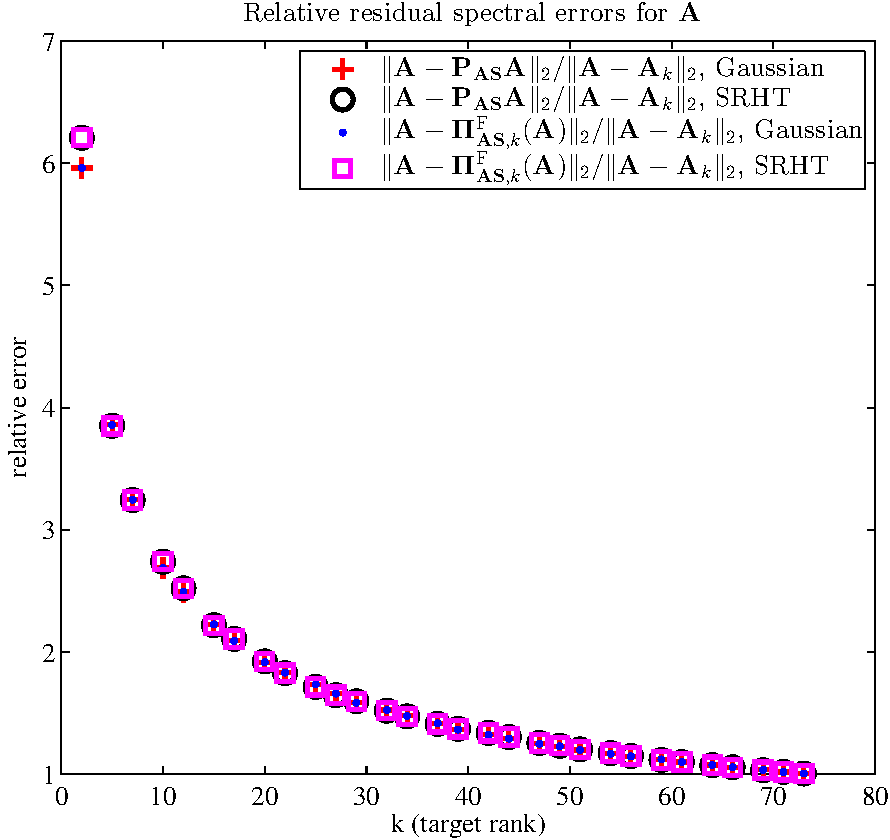
\includegraphics[width=2.8in, keepaspectratio=true]{figures/ch3/experimentA-residual-spectral.pdf}}%
 \subfigure{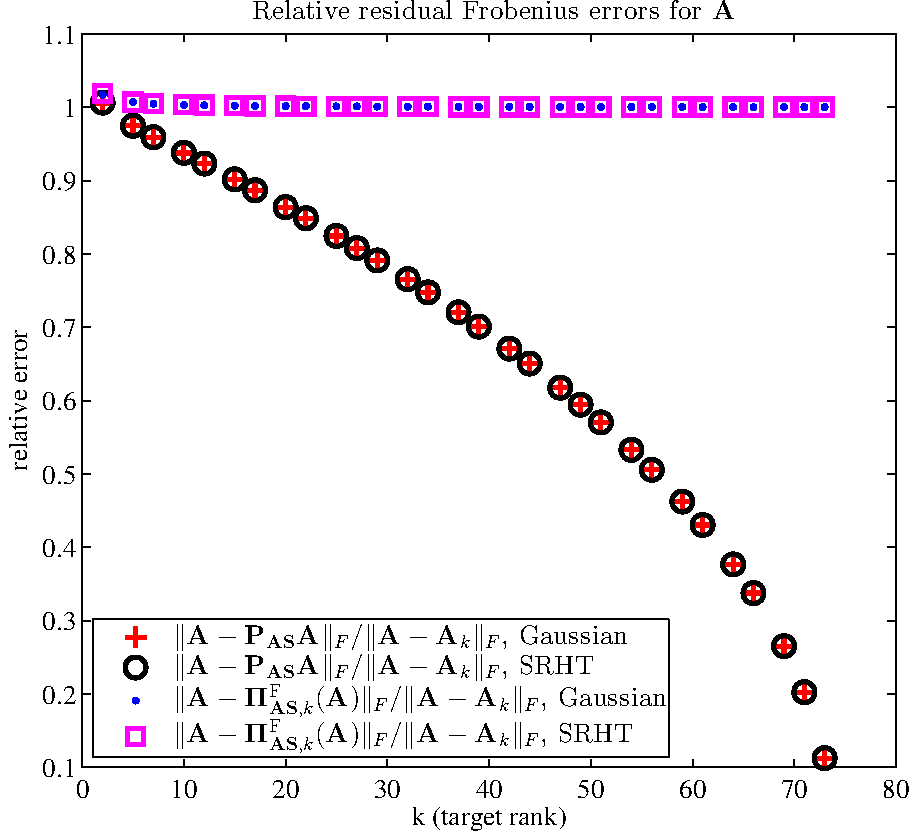
\includegraphics[width=2.8in, keepaspectratio=true]{figures/ch3/experimentA-residual-frobenius.pdf}}\\%
 \subfigure{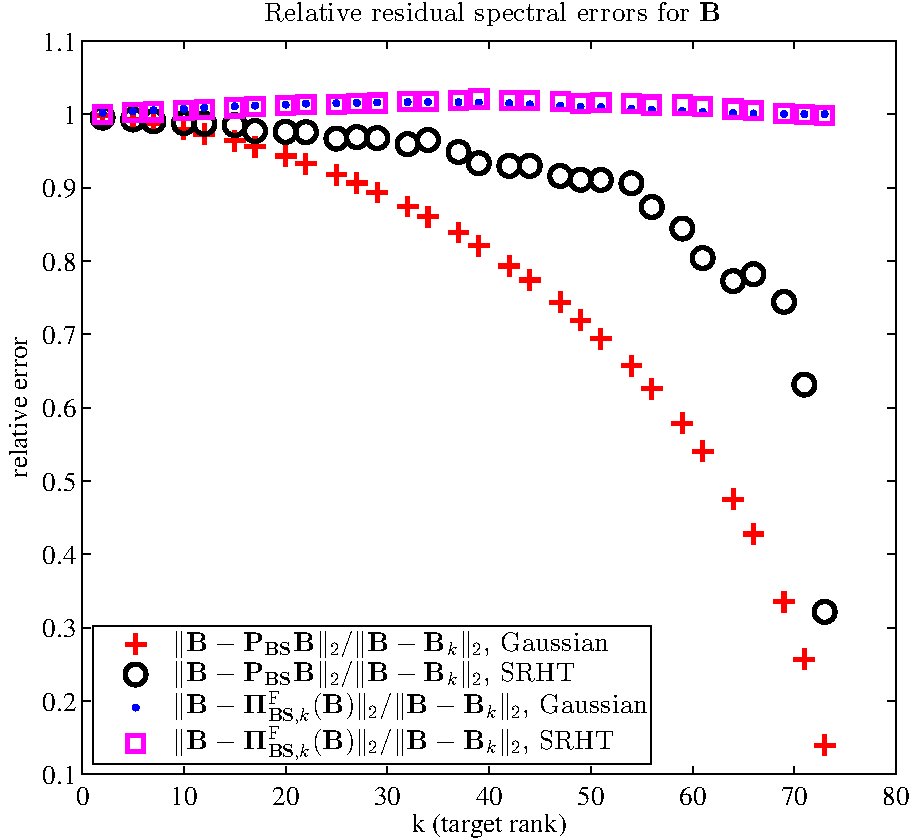
\includegraphics[width=2.8in, keepaspectratio=true]{figures/ch3/experimentB-residual-spectral.pdf}}%
 \subfigure{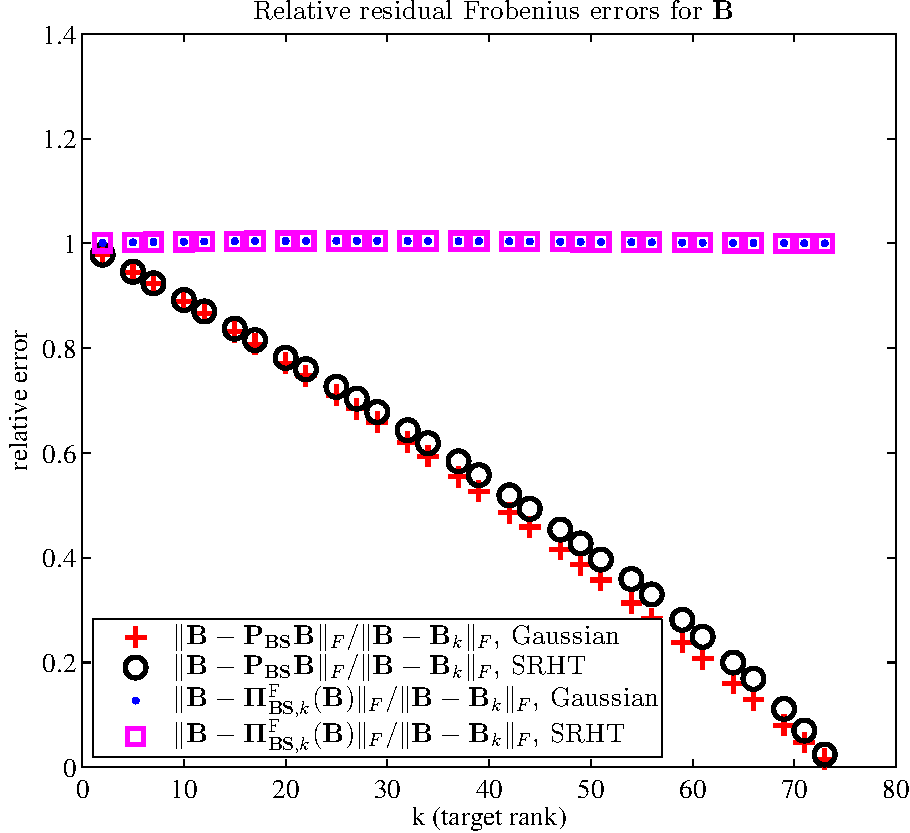
\includegraphics[width=2.8in, keepaspectratio=true]{figures/ch3/experimentB-residual-frobenius.pdf}}\\%
 \subfigure{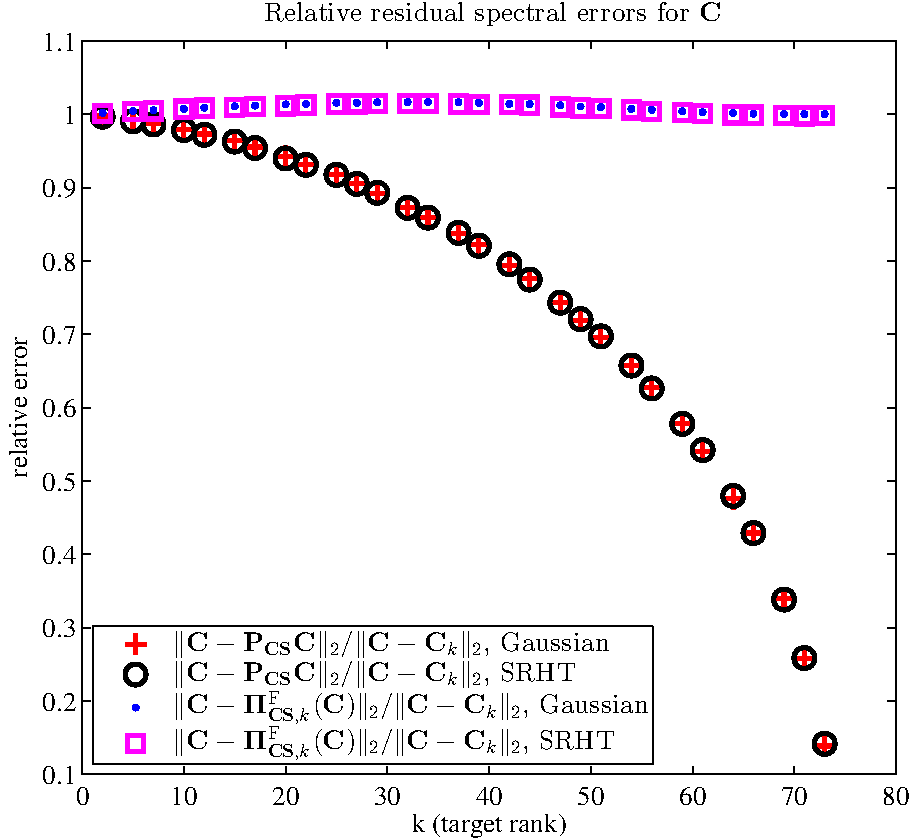
\includegraphics[width=2.8in, keepaspectratio=true]{figures/ch3/experimentC-residual-spectral.pdf}}%
 \subfigure{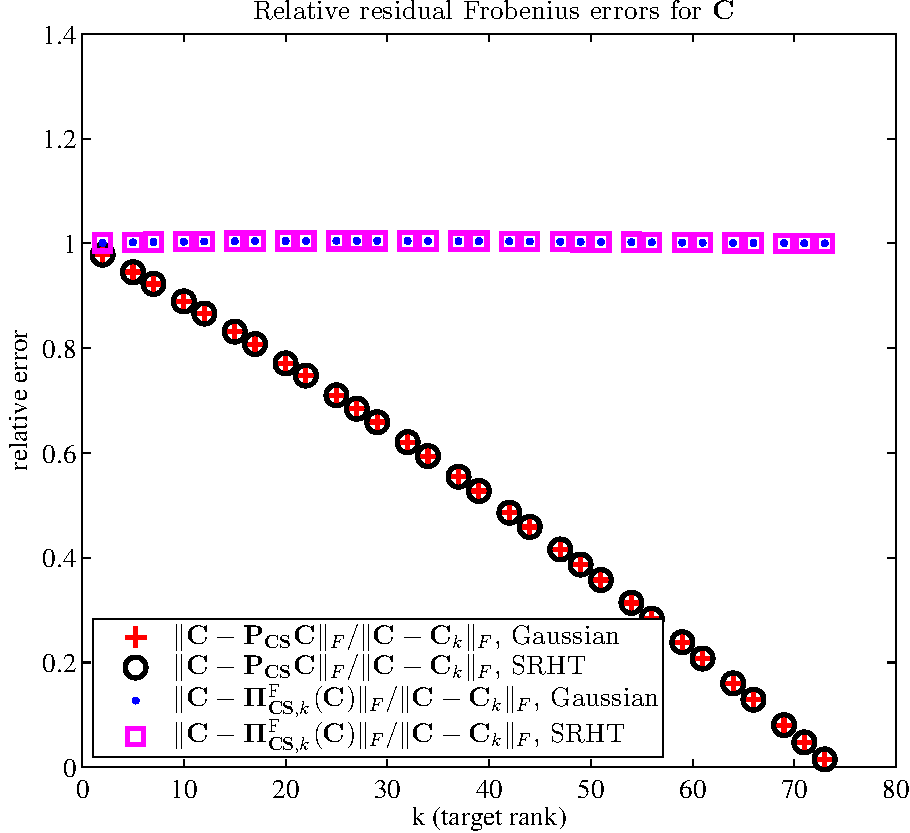
\includegraphics[width=2.8in, keepaspectratio=true]{figures/ch3/experimentC-residual-frobenius.pdf}}%
 \caption[Residual errors of low-rank approximation algorithms]{
 {\sc Residual errors of low-rank approximation algorithms.} Relative 
 spectral and Frobenius-norm residual errors of the SRHT and Gaussian low-rank approximation 
 algorithms ($\XNorm{\matM - \matP_{\matM\matS} \matM}/\XNorm{\matM - \matM_k}$ 
 and $\XNorm{\matM - \boldPi_{\matM\matS, k}^{\mathrm{F}}(\matM)}/\XNorm{\matM - \matM_k}$ 
 for $\xi = 2, \mathrm{F}$)
 as a function of the target rank $k$ for the three matrices $\matM = \matA, \matB, \matC.$ 
 Each point is the average error observed over 30 trials. 
 In each trial, $\ell = \lceil 2 k \log n \rceil$ column samples were used.}
 \label{ch3:fig:residualerrors}
\end{figure}
%
Figure~\ref{ch3:fig:residualerrors} depicts the relative residual errors of 
the Gaussian and SRHT algorithms for approximations generated using 
Algorithms~\ref{ch3:alg:nonfixedrank-randomized-svd} and~\ref{ch3:alg:fixedrank-randomized-svd}:
$\matP_{\matM\matS} \matM$ and $\boldPi_{\matM\matS, k}^{\mathrm{F}}(\matM),$ which we shall hereafter 
refer to respectively as the non-rank-restricted and rank-restricted 
approximations. Here the matrix $\matM$ is used to refer interchangeably to 
$\matA, \matB,$ and $\matC.$ The relative residual errors 
($\XNorm{\matM - \matP_{\matM\matS} \matM}/\XNorm{\matM - \matM_k}$ 
 and $\XNorm{\matM - \boldPi_{\matM\matS, k}^{\mathrm{F}}(\matM)}/\XNorm{\matM - \matM_k}$ 
 for $\xi = 2, \mathrm{F}$) shown in this figure for each value of $k$ were 
obtained by taking the average of the relative residual errors observed over 
30 trials of low-rank approximations, each formed using 
$\ell = \lceil 2 k \log n \rceil$ samples.

With the exception of the residual spectral errors on $\mat{A},$ 
which range from between two and nine times the size of the optimal rank-$k$ spectral
residual error for $k < 20,$ we see that the residual errors for all three
matrices are less than 1.1 times the residual error of $\matM_k,$ if not
significantly smaller. Specifically, the relative residual errors of the
restricted-rank approximations remain less than 1.1 over the entire range of $k$
while the relative residual errors of the non-rank-restricted approximations
actually decrease as $k$ increases.  Note that, because $\ell >k,$ the
relative errors of the non-rank-restricted approximations are often smaller
than 1, while those of the restricted-rank approximations are never smaller
than 1.

Since the matrices $\mat{B}$ and $\matC$ have the same singular values, but the
singular spaces of $\matC$ are less coherent, the difference in the residual errors of
the approximations of $\mat{B}$ and $\mat{C}$ is evidence that
the spectral-norm accuracy of the SRHT approximations is increased on less
coherent datasets; the same is true for the Frobenius norm accuracy to a lesser
extent. The Gaussian approximations seem insensitive to the level of coherence.
Only on the highly coherent matrix $\mat{B}$ do we see a notable decrease in
the residual errors when Gaussian sampling is used rather than an SRHT; however,
even in this case the residual errors of the SRHT approximations are comparable
with that of $\matB_k.$ In all, Figure~\ref{ch3:fig:residualerrors} suggests
that the gain in computational efficiency provided by the SRHT does not come at
the cost of a significant loss in accuracy and that taking $\ell = \lceil 2 k \log n
\rceil$ samples suffices to obtain approximations with small residual errors
relative to those of the optimal rank-$k$ approximations. Up to the 
specific
value of the constant, this latter observation coincides with the conclusions of
Theorems~\ref{ch3:thm:quality-of-approximation-guarantee-spectral} 
and~\ref{ch3:thm:quality-of-approximation-guarantee-Frobenius}.

\begin{figure}[htp]
 \subfigure{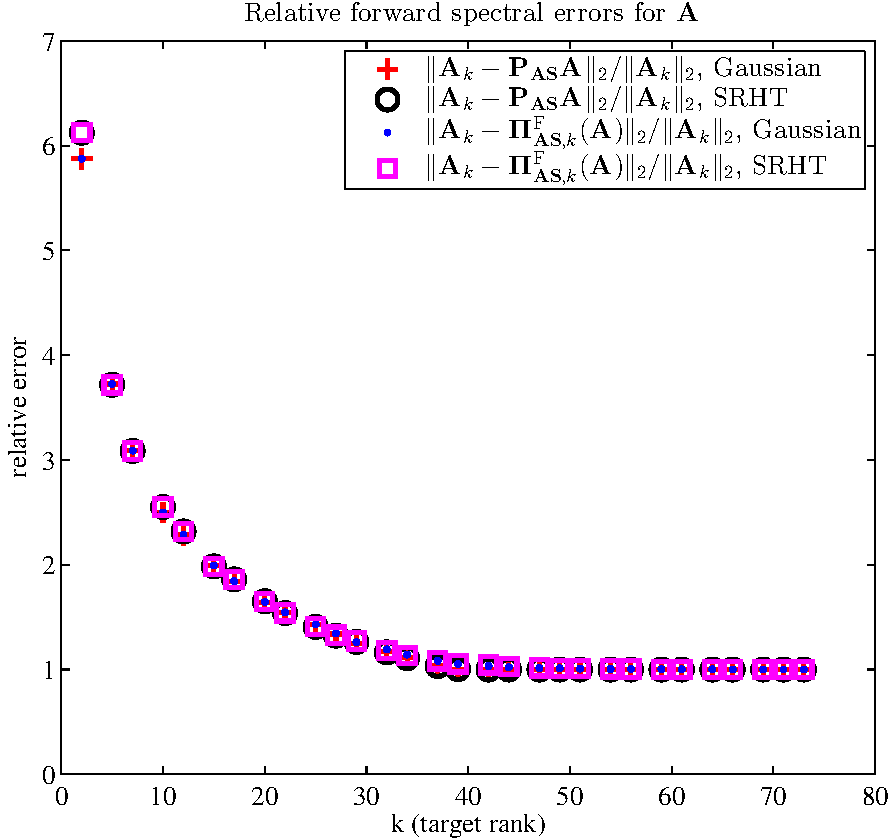
\includegraphics[width=2.8in, keepaspectratio=true]{figures/ch3/experimentA-forward-spectral.pdf}}%
 \subfigure{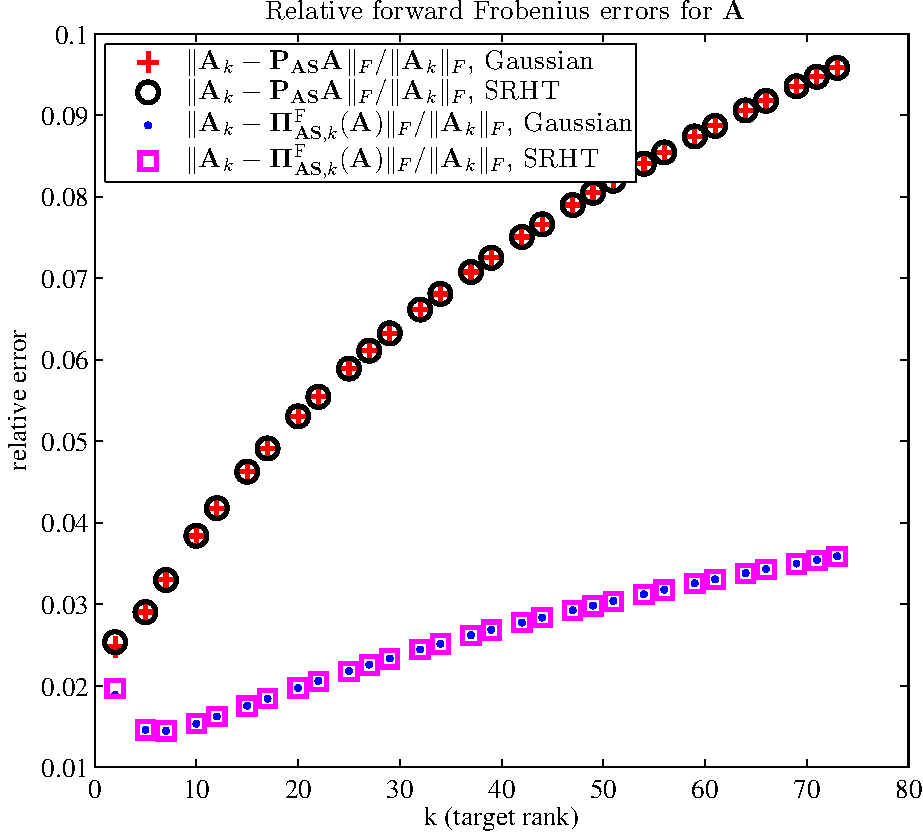
\includegraphics[width=2.8in, keepaspectratio=true]{figures/ch3/experimentA-forward-frobenius.pdf}}\\%
 \subfigure{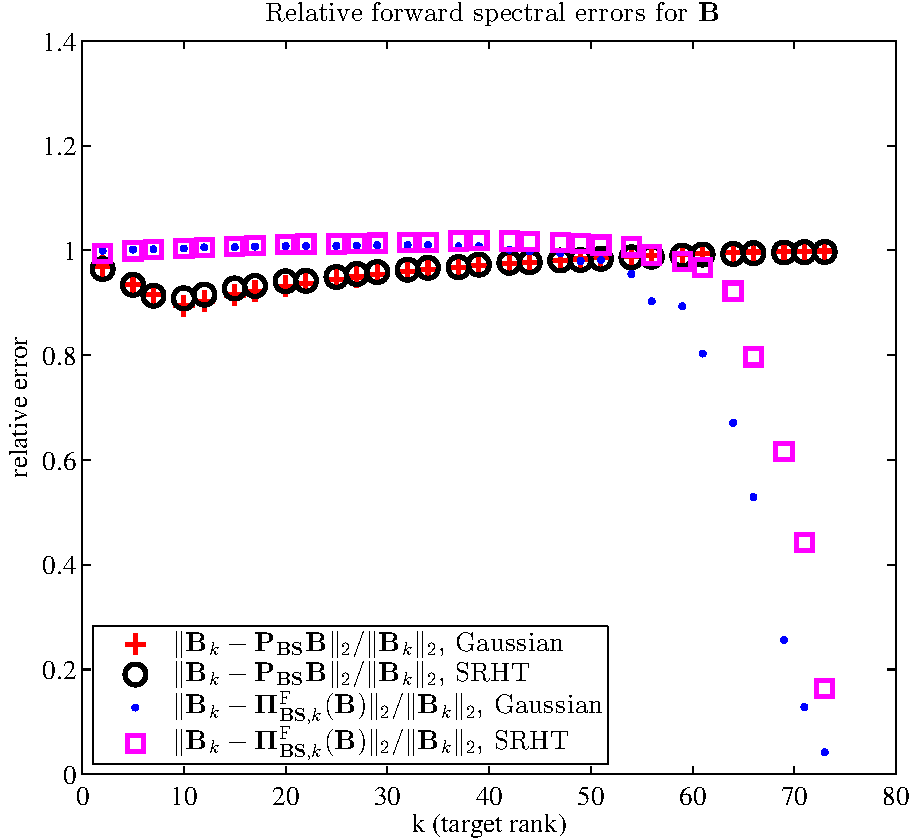
\includegraphics[width=2.8in, keepaspectratio=true]{figures/ch3/experimentB-forward-spectral.pdf}}%
 \subfigure{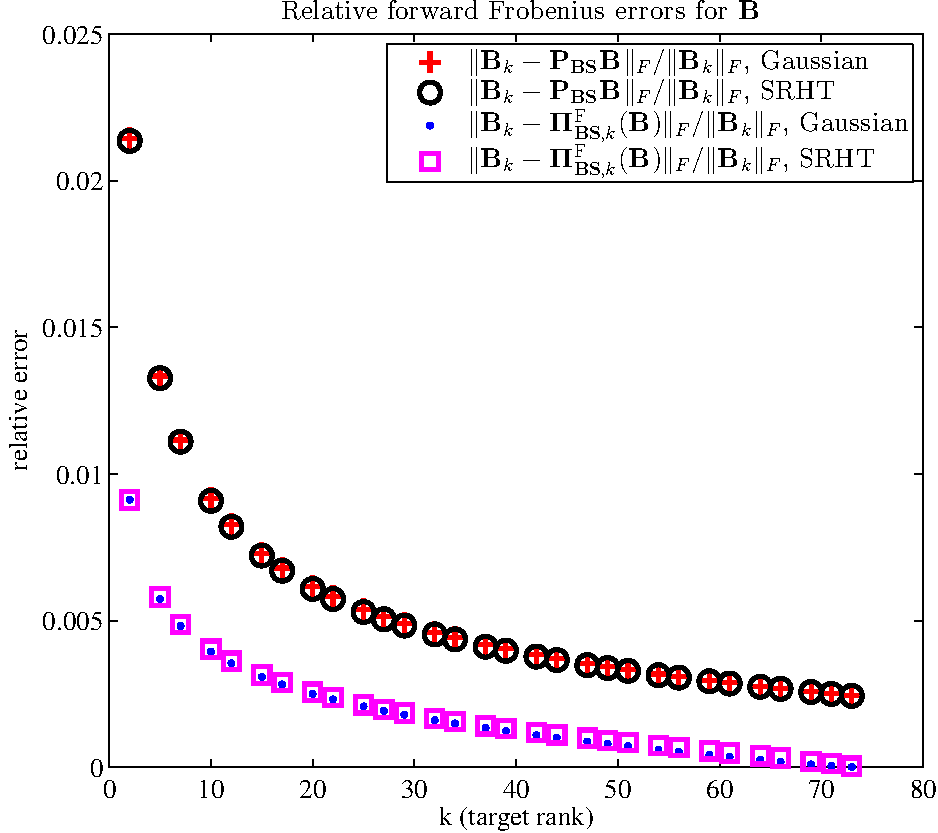
\includegraphics[width=2.8in, keepaspectratio=true]{figures/ch3/experimentB-forward-frobenius.pdf}}\\%
 \subfigure{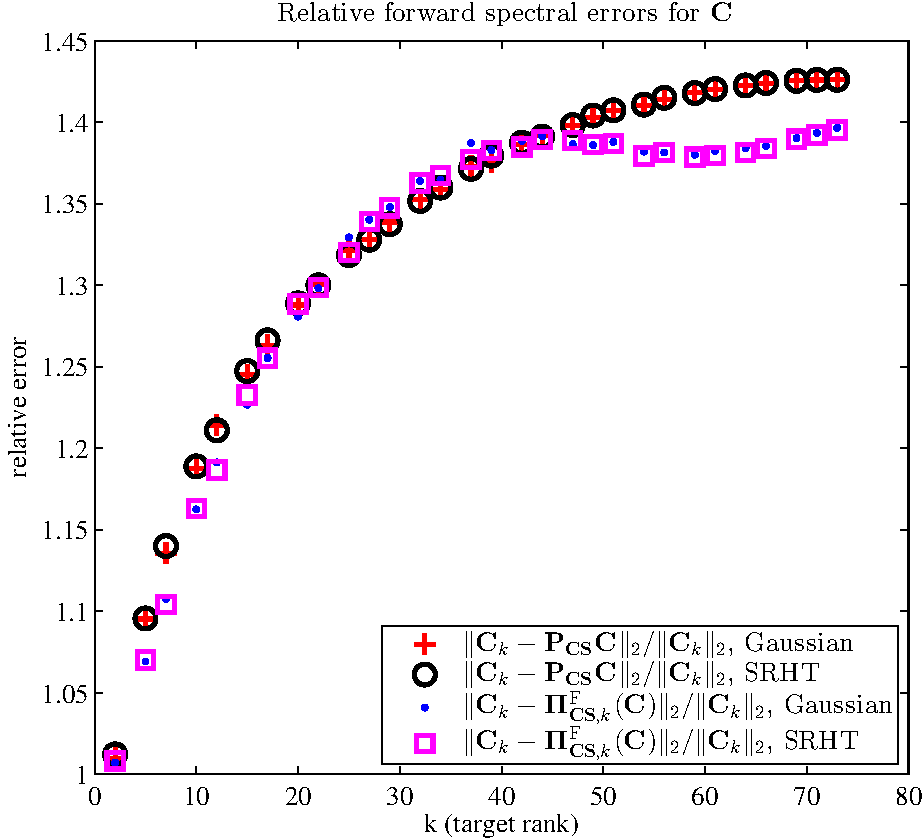
\includegraphics[width=2.8in, keepaspectratio=true]{figures/ch3/experimentC-forward-spectral.pdf}}%
 \subfigure{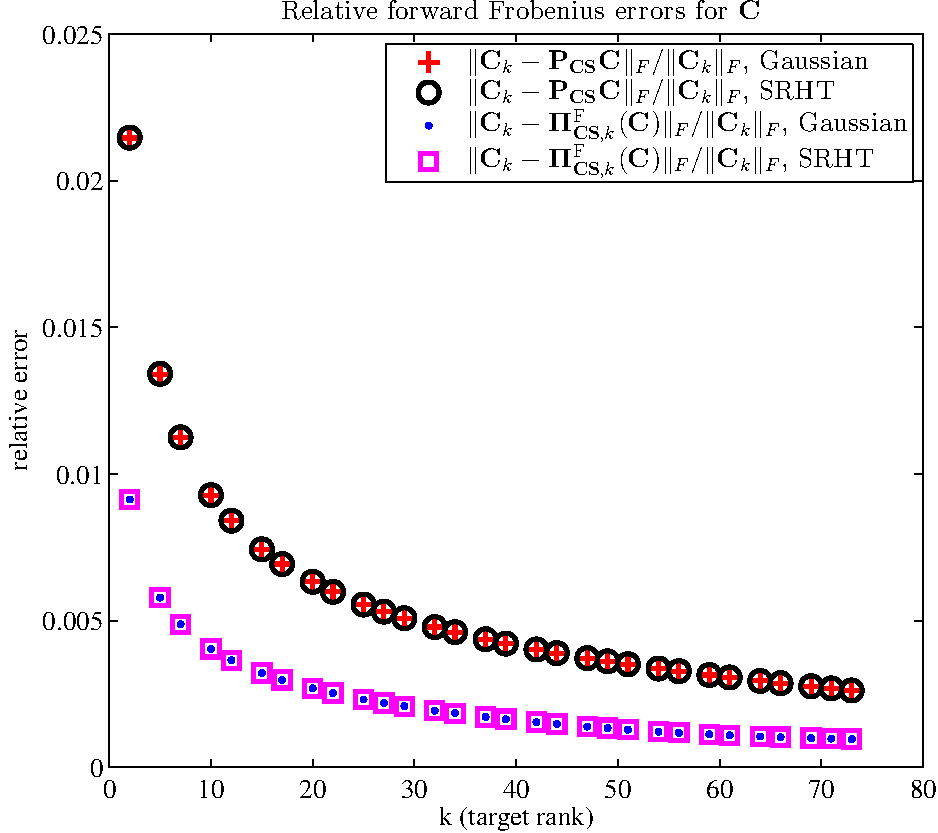
\includegraphics[width=2.8in, keepaspectratio=true]{figures/ch3/experimentC-forward-frobenius.pdf}}%
 \caption[Forward errors of low-rank approximation algorithms]{
 {\sc Forward errors of low-rank approximation algorithms.} The 
 relative spectral and Frobenius-norm forward errors of the SRHT and Gaussian low-rank approximation algorithms
 ($\XNorm{\matM_k - \matP_{\matM\matS} \matM}/\XNorm{\matM - \matM_k}$ 
 and $\XNorm{\matM_k - \boldPi_{\matM\matS, k}^{\mathrm{F}}(\matM)}/\XNorm{\matM - \matM_k}$ 
 for $\xi = 2, \mathrm{F}$)
 as a function of the target rank $k$ for the three matrices $\matM = \matA, \matB, \matC.$ Each point is the average of the errors observed over 30 trials.
 In each trial, $\ell = \lceil 2 k \log n \rceil$ column samples were used.}
 \label{ch3:fig:forwarderrors}
\end{figure}

Figure~\ref{ch3:fig:forwarderrors} depicts the relative forward errors of the
Gaussian and SRHT algorithms ($\XNorm{\matM_k - \matP_{\matM\matS} \matM}/\XNorm{\matM - \matM_k}$ 
 and $\XNorm{\matM_k - \boldPi_{\matM\matS, k}^{\mathrm{F}}(\matM)}/\XNorm{\matM - \matM_k}$ 
 for $\xi = 2, \mathrm{F}$) for the
non-rank-restricted and rank-restricted approximations. The error shown for each
$k$ is the average relative forward error observed over 30 trials of low-rank
approximations each formed using $\ell = \lceil 2 k \log n\rceil$ samples. We
observe that the forward errors of both algorithms for both choices of sampling
matrices are on the scale of the norm of $\mat{M}_k.$ By looking at the relative
spectral-norm forward errors we see that in this norm, perhaps contrary to
intuition, the rank-restricted approximation does not provide a more accurate
approximation to $\matM_k$ than does the non-rank-restricted approximation.
However the rank-restricted approximation clearly provides a more accurate
approximation to $\matM_k$ than the non-rank-restricted 
approximation in the
Frobenius norm. A rather
unexpected observation is that the rank-restricted approximations are more
accurate in the spectral norm for highly coherent matrices ($\matB$) than they
are for matrices which are almost minimally coherent ($\matC$). Overall,
Figure~\ref{ch3:fig:forwarderrors} suggests that the SRHT low-rank approximation
algorithms provide accurate approximations to $\matM_k$ when $\ell$ is in the
regime suggested by Theorems~\ref{ch3:thm:quality-of-approximation-guarantee-spectral}
and~\ref{ch3:thm:quality-of-approximation-guarantee-Frobenius}.

\begin{figure}
 \centering
 \subfigure{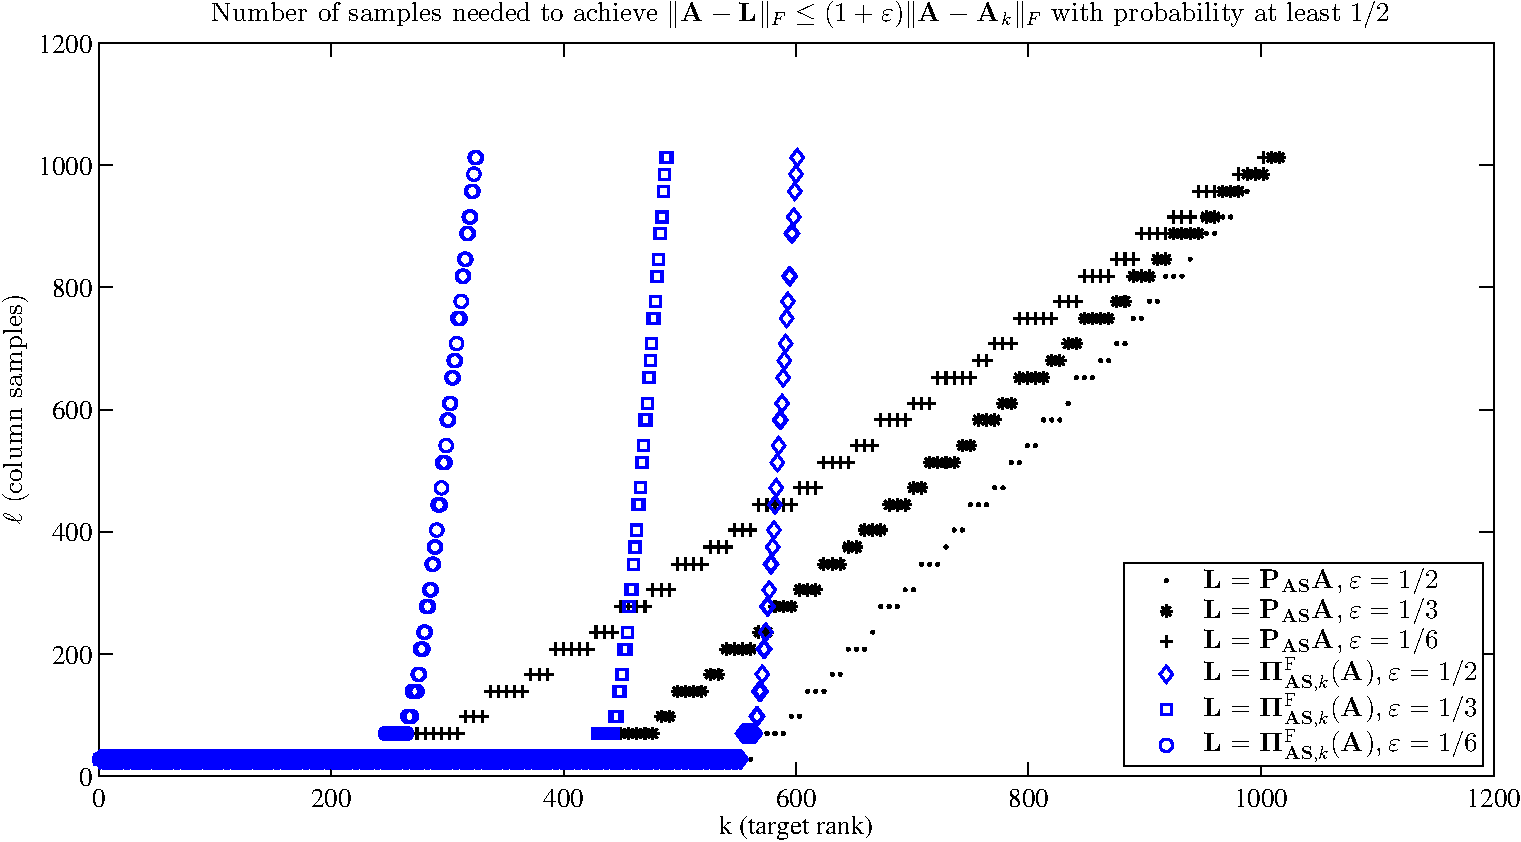
\includegraphics[width=4.9in, keepaspectratio=true]{figures/ch3/experimentA-empirically-necessary-r.pdf}}\\%
 \subfigure{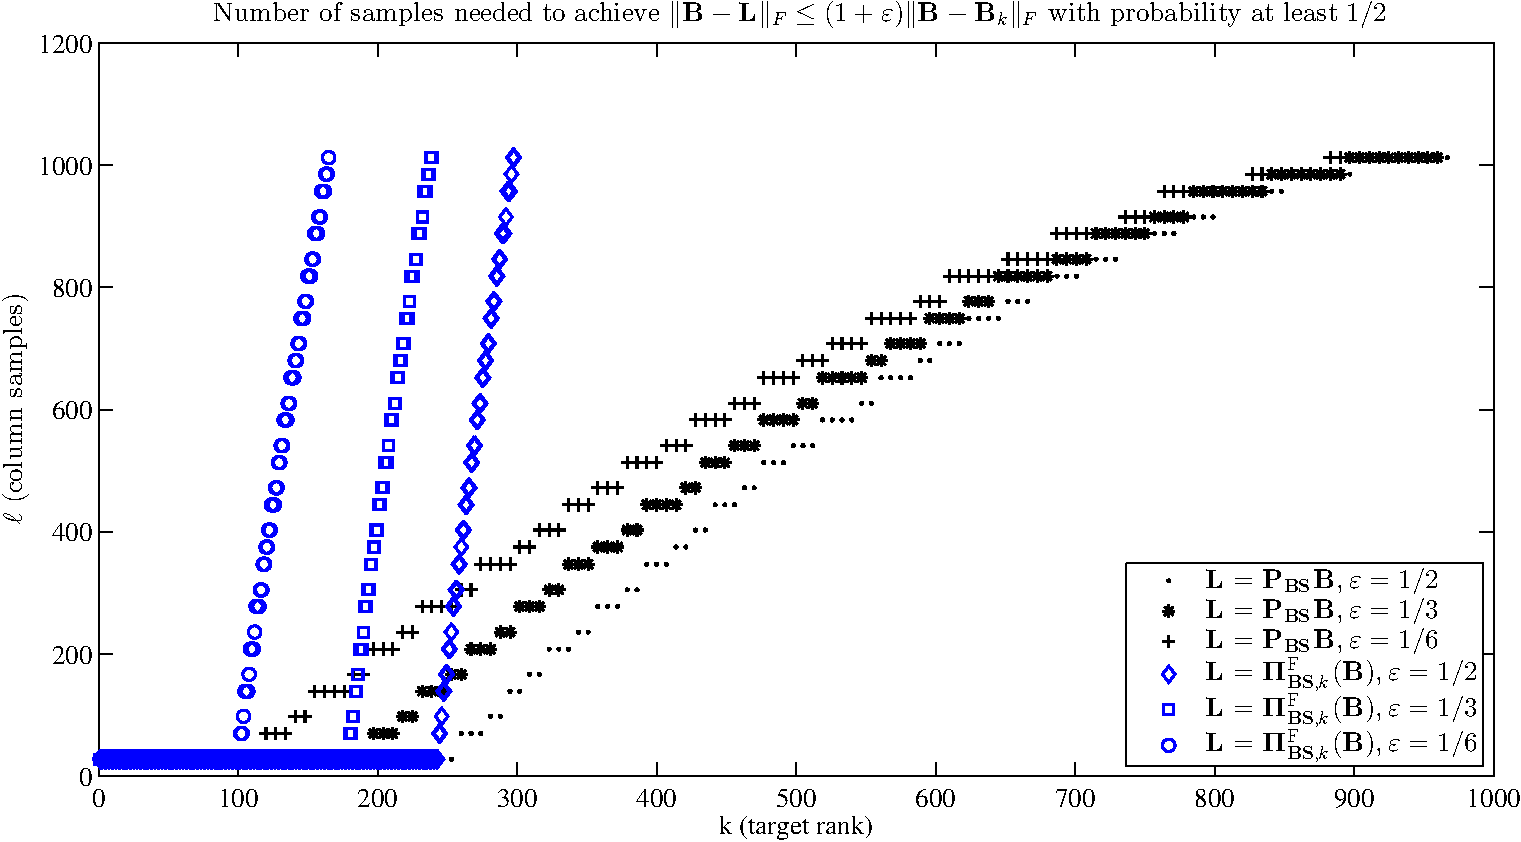
\includegraphics[width=4.9in, keepaspectratio=true]{figures/ch3/experimentB-empirically-necessary-r.pdf}}\\%
 \subfigure{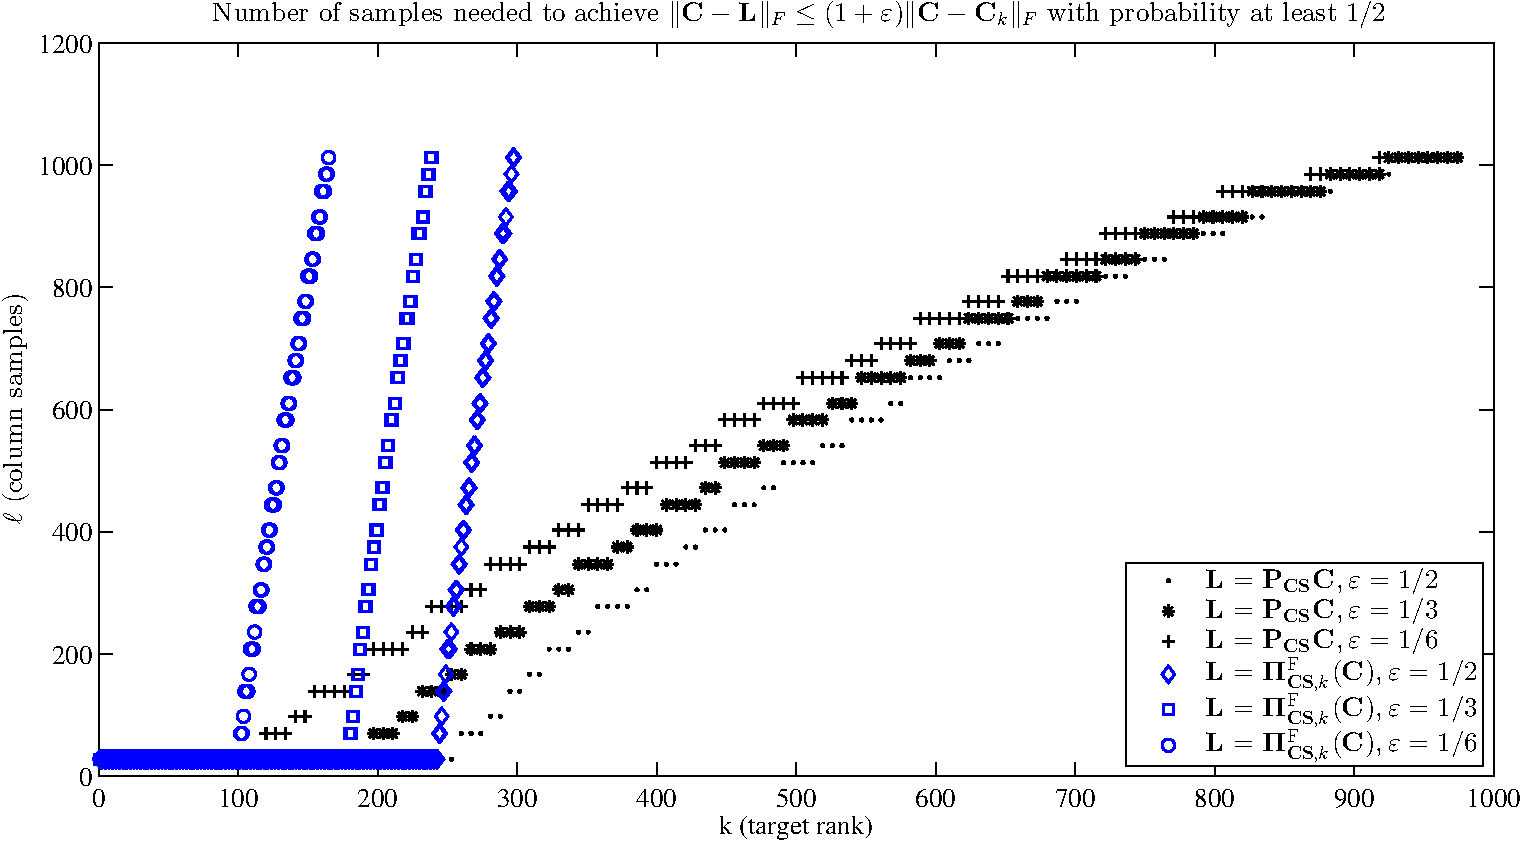
\includegraphics[width=4.9in, keepaspectratio=true]{figures/ch3/experimentC-empirically-necessary-r.pdf}}
 \caption[The number of column samples required for relative error Frobenius-norm approximations]{
 {\sc The number of column samples required for relative error Frobenius-norm approximations.} The 
 value of $\ell$ empirically necessary to ensure that, with probability at least one-half, approximations generated
 by the SRHT algorithms satisfy $\FNorm{\matM - \matP_{\matM\matTh\transp} \matM} \leq (1 + \epsilon) \FNorm{\matM - \matM_k}$ and 
 $\FNorm{\matM - \boldPi_{\matM\matTh\transp, k}^{\mathrm{F}}(\matM)} \leq (1 + \epsilon) \FNorm{\matM - \matM_k}$ (for $\matM = \matA, \matB, \matC$).}
 \label{ch3:fig:empiricalrnecessary}
\end{figure}

\subsection{Empirical evaluation of our error bounds}
Figures~\ref{ch3:fig:residualerrors} and~\ref{ch3:fig:forwarderrors} show that when 
$\ell = \lceil 2 k \log n \rceil$ samples are taken, the SRHT low-rank approximation algorithms 
both provide approximations to $\matM$ that are within a factor of $1 + \epsilon$ as 
accurate in the Frobenius norm as $\matM_k,$ as Theorem~\ref{ch3:thm:quality-of-approximation-guarantee-Frobenius} 
suggests should be the case. More precisely, Theorem~\ref{ch3:thm:quality-of-approximation-guarantee-Frobenius} 
assures us that $528 \epsilon^{-1} [\sqrt{k} + \sqrt{8 \log(8 n/\delta)}]^2 \log(8k/\delta)$ column 
samples are sufficient to ensure that, with at least probability $1 - \delta$, $\matP_{\matM \matTh\transp} \matM$ 
and $\boldPi_{\matM\matTh\transp, k}^{\mathrm{F}}(\matM)$ have Frobenius norm residual and forward error 
within $1 + \epsilon$ 
of that of $\matM_k.$ The factor $528$ can certainly be reduced by optimizing the numerical 
constants given in Theorem~\ref{ch3:thm:quality-of-approximation-guarantee-Frobenius}. 
But what is the smallest $\ell$ that ensures the
Frobenius norm residual error bounds 
$\FNorm{\matM - \matP_{\matM\matTh\transp} \matM} \leq (1 + \epsilon) \FNorm{\matM - \matM_k}$ and 
 $\FNorm{\matM - \boldPi_{\matM\matTh\transp, k}^{\mathrm{F}}(\matM)} \leq (1 + \epsilon) \FNorm{\matM - \matM_k}$ are 
satisfied with some fixed probability? To investigate, in Figure~\ref{ch3:fig:empiricalrnecessary} 
we plot the values of $\ell$ determined empirically to be sufficient to obtain $(1+\epsilon)$ 
Frobenius norm residual errors relative to the optimal rank-$k$ approximation; we fix the 
failure probability $\delta=1/2$ and vary $\epsilon.$ Specifically, the $\ell$ plotted for
each $k$ is the smallest number of samples for which 
$\FNorm{\matM - \matP_{\matM\matTh\transp} \matM} \leq (1 + \epsilon) \FNorm{\matM - \matM_k}$ 
or $\FNorm{\matM - \boldPi_{\matM\matTh\transp, k}^{\mathrm{F}}(\matM)} \leq (1 + \epsilon) \FNorm{\matM - \matM_k}$
in at least 15 out of 30 trials.

It is clear that, for fixed $k$ and $\epsilon,$ the number of samples $\ell$ required 
to form a non-rank-restricted approximation to $\matM$ with $1+\epsilon$ relative 
residual error is smaller than the $\ell$ required to form a rank-restricted approximation 
with $1+\epsilon$ relative residual error. Note that for small values of $k$, the 
$\ell$ necessary for relative residual error to be achieved is actually smaller than $k$ for 
all three datasets. This is a reflection of the fact that when $k_1 < k_2$ are small, the 
ratio $\FNorm{\matM - \matM_{k_2}}/\FNorm{\matM - \matM_{k_1}}$ is very close to one. Outside 
of the initial flat regions, the empirically determined value of $r$ seems to grow linearly with $k$;
this matches with the observation of Woolfe et al. that taking $\ell=k+8$ suffices to 
consistently form accurate low-rank approximations using the SRFT scheme, which is 
very similar to the SRHT scheme~\cite{WLRT08}. We also note that this matches with 
Theorem~\ref{ch3:thm:quality-of-approximation-guarantee-Frobenius}, which predicts that the 
necessary $\ell$ grows at most linearly with $k$ with a slope like $\log n.$

Finally, Theorem~\ref{ch3:thm:quality-of-approximation-guarantee-spectral} does \emph{not} guarantee 
that $1+\epsilon$ spectral-norm relative residual errors can be achieved. Instead, it 
provides bounds on the spectral-norm residual errors achieved in terms of 
$\TNorm{\matM - \matM_k}$ and $\FNorm{\matM - \matM_k}$ that are guaranteed to hold when 
$\ell$ is sufficiently large. In Figure~\ref{ch3:fig:predictedspecerrvsactual} we compare the 
spectral-norm residual error guarantees of Theorem~\ref{ch3:thm:quality-of-approximation-guarantee-spectral} 
to what is achieved in practice. To do so, we take the optimistic viewpoint that the constants 
in Theorem~\ref{ch3:thm:quality-of-approximation-guarantee-spectral} can be optimized to unity. Under 
this view, if more columns than $\ell_2 = \epsilon^{-1} [\sqrt{k} + \sqrt{\log(n/\delta)}]^2 \log(k/\delta)$ 
are used to construct the SRHT approximations, then the spectral-norm residual error is no larger than
\[
 b_2 = \left(1 + \sqrt{\frac{\log(n/\delta) \log(\rho/\delta)}{\ell}}\right) \cdot 
 \TNorm{\matM - \matM_k} + \sqrt{\frac{\log(\rho/\delta)}{\ell}} \cdot \FNorm{\matM - \matM_k},
\]
where $\rho$ is the rank of $\matM,$ with probability greater than $1-\delta.$ Our comparison consists of 
using $\ell_2$ samples to construct the SRHT approximations and then comparing the predicted upper bound on 
the spectral-norm residual error, $b_2$, to the empirically observed spectral-norm residual errors. 
Figure~\ref{ch3:fig:predictedspecerrvsactual} shows, for several values of $k$, the upper bound $b_2$ and 
the observed relative spectral-norm residual errors, with precision parameter $\epsilon = 1/2$ and 
failure parameter $\delta = 1/2.$ For each value of $k,$ the empirical spectral-norm residual error plotted 
is the average of the errors over 30 trials of low-rank approximations. Note from 
Figure~\ref{ch3:fig:predictedspecerrvsactual} that with this choice of $\ell,$ the spectral-norm residual errors 
of the rank-restricted and non-rank-restricted SRHT approximations are essentially the same.

\begin{figure}
 \centering
 \subfigure{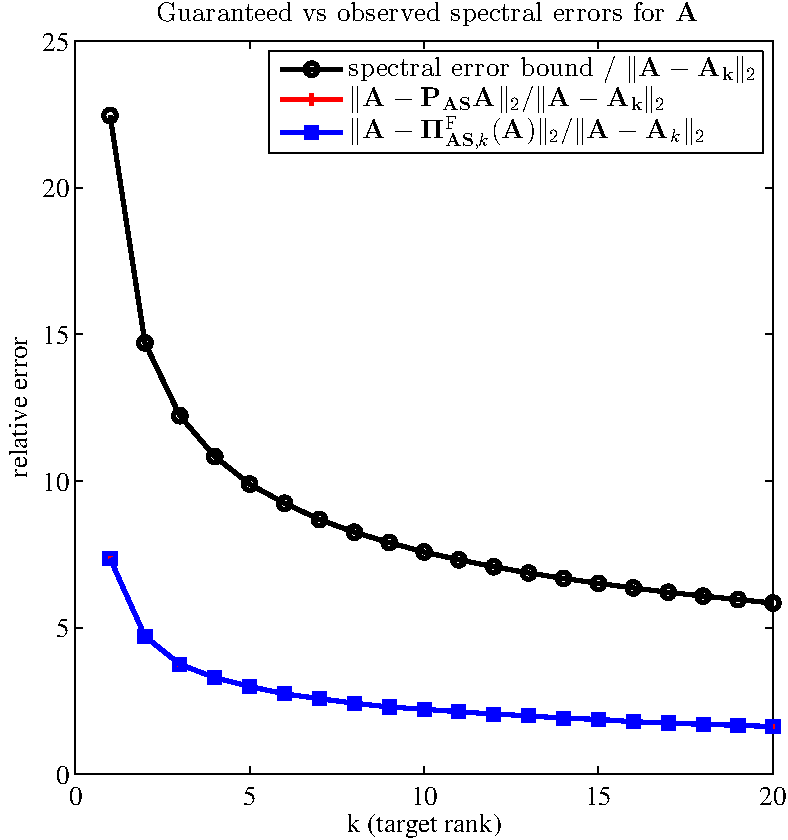
\includegraphics[width=2in, keepaspectratio=true]{figures/ch3/experimentA-actual-versus-predicted-spectral-error}}%
 \subfigure{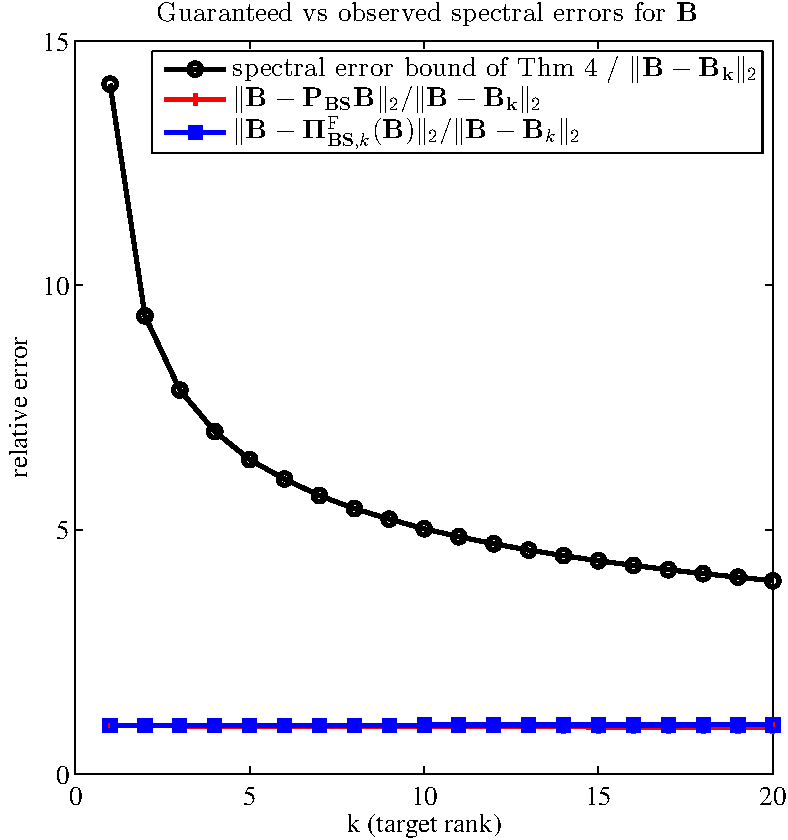
\includegraphics[width=2in, keepaspectratio=true]{figures/ch3/experimentB-actual-versus-predicted-spectral-error}}%
 \subfigure{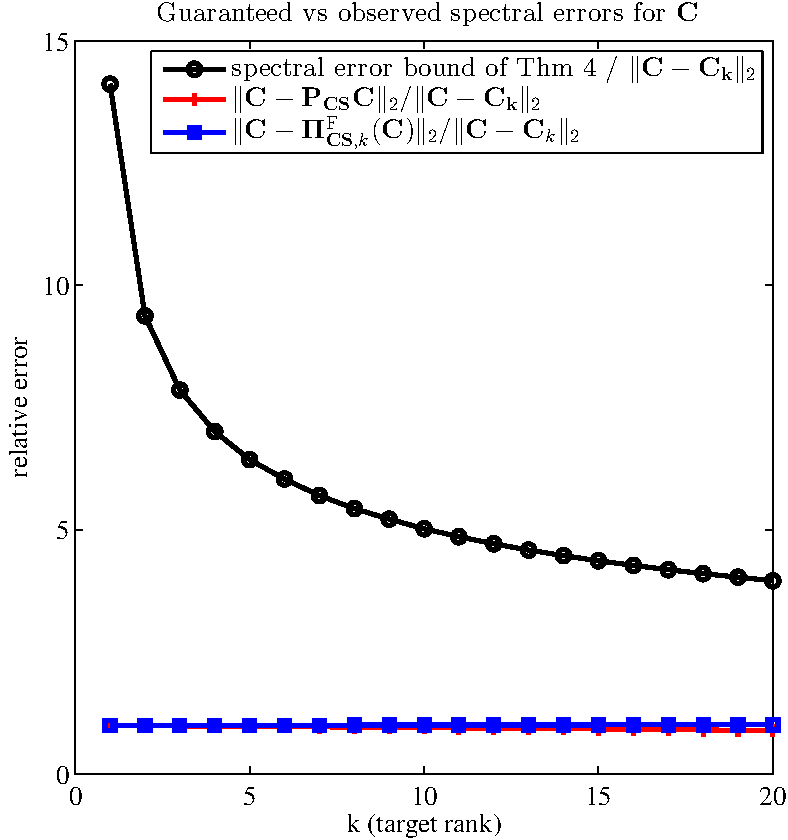
\includegraphics[width=2in, keepaspectratio=true]{figures/ch3/experimentC-actual-versus-predicted-spectral-error}}
 \caption[Empirical versus predicted spectral-norm residual errors of low-rank approximations]{%
 {\sc Empirical versus predicted spectral-norm residual errors of low-rank approximations.} The empirical spectral-norm residual errors relative to those of the optimal rank-$k$ approximants 
 ($\TNorm{\matM - \matP_{\matM\matTh\transp} \matM}/\|\matM - \matM_k\|_2$ and 
 $\|\matM - \boldPi_{\matM\matTh\transp,k}^{\mathrm{F}}(\matM)\|_2/\|\matM - \matM_k\|_2$) plotted alongside the same ratio for the bounds given in 
 Theorem~\ref{ch3:thm:quality-of-approximation-guarantee-spectral}, when $\ell = \lceil 2[\sqrt{k} + \sqrt{\log(2n)}]^2 \log(2k) \rceil$ 
 (for $\matM = \matA, \matB, \matC$). On the scale shown, the errors of the two SRHT-based approximation algorithms are essentially identical.}
 \label{ch3:fig:predictedspecerrvsactual}
\end{figure}

Judging from Figures~\ref{ch3:fig:empiricalrnecessary} and~\ref{ch3:fig:predictedspecerrvsactual}, even when we
assume the constants present can be optimized away, the bounds given in Theorems~\ref{ch3:thm:quality-of-approximation-guarantee-spectral}
and~\ref{ch3:thm:quality-of-approximation-guarantee-Frobenius}
are pessimistic: it seems that in fact approximations with Frobenius-norm residual error within $1+\epsilon$ of the error of the
optimal rank-$k$ approximation can be obtained with $\ell$ linear in $k,$ and the spectral-norm residual errors are smaller than the supplied upper bounds.
Thus there is still room for improvement in our understanding of the SRHT low-rank approximation algorithm, but as explained in Section~\ref{ch3:sec:priorwork},
ignoring constants, the bounds of Theorem~\ref{ch3:thm:quality-of-approximation-guarantee-spectral} are often tighter than those obtained in earlier works.

To bring perspective to this discussion, consider that even if one limits consideration to deterministic algorithms, the
known error bounds for the Gu--Eisenstat rank-revealing QR---a popular and widely used algorithm for low-rank 
approximation---are quite pessimistic and do not reflect the excellent accuracy that is seen in practice~\cite{GE96}. 
Regardless, we do not advocate using these approximation schemes for applications in which highly accurate low-rank 
approximations are needed. Rather, Theorems~\ref{ch3:thm:quality-of-approximation-guarantee-spectral} 
and~\ref{ch3:thm:quality-of-approximation-guarantee-Frobenius} and our numerical experiments 
suggest that they are appropriate in situations where one is willing to trade some accuracy for a gain in computational efficiency.
